\documentclass[11pt,doublespace]{unhthesis}

\usepackage{custom}
\hyphenation{gno-mon-ly}


\begin{document}

\title{DEVELOPMENT OF A HIGH-INTEGRITY ANALYTICAL AND EXPERIMENTAL TEST BED FOR OBSERVER-BASED CONTROLLERS FOR NASA's MAGNETOSPHERIC MULTISCALE MISSION SPACECRAFT}
\author{Daniel R. Couture}
\prevdegrees{B.S. Mechanical Engineering, University of New Hampshire (2001)}
\major{Mechanical Engineering}
\degree{Master of Science}
\degreemonth{May}
\degreeyear{2014}
\thesisdate{March 15, 2014}
\DOCUMENTtype{THESIS}
\Documenttype{Thesis}
\documenttype{thesis}
\maketitle

\copyrightyear{2014}
\makecopyright

\supervisor{Dr. May-Win L. Thein}{Associate Professor of Mechanical Engineering}
\committee{Dr. Barry Fussell}{Professor of Mechanical Engineering}
\committee{Philip J. Hatcher}{Professor of Computer Science}
\makeapproval



\thispagestyle{empty}
\noindent This thesis has been examined and approved.
\vspace*{2.5cm}

\begin{minipage}{0.2\textwidth}
        \begin{flushleft}
        \end{flushleft}
    \end{minipage}
\begin{minipage}{0.8\textwidth}
        \begin{flushleft}
            \underline{\hspace{10cm}} \\
            Thesis Director, Dr. May-Win L. Thein\\
            Associate Professor of Mechanical Engineering\\
            \vspace{1.5cm}
            \underline{\hspace{10cm}} \\
            Dr. Barry Fussell\\
            Professor of Mechanical Engineering\\
            \vspace{1.5cm}
            \underline{\hspace{10cm}} \\
            \TODO{Find third professor}
            \vspace{2cm}
            \hspace{3cm}\underline{\hspace{7cm}} \\
            \hspace{3cm}Date
        \end{flushleft}
\end{minipage}\\[1cm]

\pagebreak

\linespread{1}

\addcontentsline{toc}{chapter}{Acknowledgements}
\begin{center}
\textbf{\large Acknowledgements}
\end{center}


I would like to fin ack

%\chapter*{Acknowledgements}
%\addcontentsline{toc}{chapter}{Acknowledgements}
%\label{chap:acknowledgements}


\pagebreak
\tableofcontents


\pagebreak
\addcontentsline{toc}{chapter}{List of Tables}
\label{chap:tables}
\listoftables


\pagebreak
\addcontentsline{toc}{chapter}{List of Figures}
\label{chap:figues}
\listoffigures

\pagebreak
\addcontentsline{toc}{chapter}{Nomenclature}


\nomenclature[Q]{$\bs{q_n}$}{nutation quaternion}
\nomenclature[Q]{$\bs{q}$}{quaternion where $\bs{q} = q_1\bs{i}+q_2\bs{j}+q_3\bs{k}+q_0$}
\nomenclature[Q]{$\bs{q_k}$}{quaternion state at discrete step $k$}
\nomenclature[Q]{$\bs{q_r}$}{rotational quaternion}
\nomenclature[Q]{$\bs{q_I}$}{identity quaternion where $\bs{q_I} = 0\bs{i}+0\bs{j}+0\bs{k}+1$}
\nomenclature[M]{$\bs{\Omega}$}{skew symmetric matrix}
\nomenclature[B]{$\bs{\omega}$}{Body Rate}

\printnomenclature


% \begin{tabular}{|l|c|c|}
%   \hline
%   % after \\: \hline or \cline{col1-col2} \cline{col3-col4} ...
%  \T \B \bf{Variable Name} & \bf{Symbol} & \bf{Units} \\ \hline
%  \T \B   Full quaternion & $\bf{\bar{q}}$ & -  \\ \hline
%  \T \B Quaternion imaginary vector & $\bf{q}$ & -  \\ \hline
%  \T \B Quaternion scalar component & $\bf{q_0}$ & -  \\ \hline
%  \T \B Spacecraft angular rates & $\boldsymbol{\omega}$ & $rad/s$  \\ \hline
%  \T \B Time derivative of full quaternion & $\bf{\dot{\bar{q}}}$ & -   \\ \hline
%  \T \B Time derivative of spacecraft angular rates & $\boldsymbol{\dot{\omega}}$ & $rad/s^2$   \\ \hline
% \multirow{2}{*} \T \B Angular rate augmented with zero for quaternion& $\boldsymbol{\bar{\omega}_{b/o}}$ & $rad/s^2$   \\
%      operators  & &  \\  \hline
% % \T \B Acceleration at expected location of accelerometer & $\bf{a}_{nom}$ & $m/s^2$  \\ \hline
%  \T \B True acceleration at location of accelerometer & $\boldsymbol{a}_{true}$ &  $m/s^2$   \\ \hline
% \multirow{2}{*} \T \B Acceleration where accelerometer is thought  & {$\boldsymbol{a_{nom}}$} &  $m/s^2$ \\
%     to be and oriented & & \\ \hline
%  \T \B Measured acceleration ($a_{true}$ + noise) & $\boldsymbol{a_m}$ & $m/s^2$  \\ \hline
% \multirow{2}{*} \T \B Acceleration at true accelerometer location,  & $\boldsymbol{a_{shift}}$ & $m/s^2$  \\
%    aligned to body axis & & \\ \hline
% \multirow{2}{*} \T \B Acceleration at true accelerometer location, & $\boldsymbol{a_{mis}}$ & $m/s^2$  \\
%      aligned to accelerometer axis & & \\ \hline
%  \T \B Accelerometer sensor bias & $\boldsymbol{a_b}$ & $m/s^2$  \\ \hline
% \multirow{2}{*} \T \B Shift in accelerometer location from measured & $\boldsymbol{\delta r}$  & $m$  \\
%    location   & &  \\ \hline
% \multirow{2}{*} \T \B accelerometer axes orthogonal rotation defined & $\boldsymbol{\delta}$  & $rad$  \\
%     by a small angle 1-2-3 Euler angle sequence & & \\ \hline
% \multirow{2}{*} \T \B Rotation matrix defining accelerometer axes  & $\boldsymbol{\Delta}$  & -  \\
%     orthogonal rotation & & \\  \hline
%  \T \B Lumped bias correction term & $\boldsymbol{a}_{LB}$  & $m/s^2$  \\ \hline
%  \T \B Spacecraft true inertia tensor & $\boldsymbol{J}$ & $kg-m^2$  \\ \hline
%  \T \B Nominal (model) spacecraft inertia tensor & $\boldsymbol{\hat{J}}$ & $kg-m^2$  \\ \hline
%  \T \B Measured accelerometer location prior to launch &  $\boldsymbol{r}$ & $m$  \\ \hline
%  \T \B Accelerometer white noise & $\boldsymbol{\nu}_{accelerometer}$ & $m/s^2$  \\ \hline
%  \T \B Torques on spacecraft & $\boldsymbol{T}$ & $N-m$  \\ \hline
%  \T \B State covariance matrix & $\boldsymbol{Q}$ & -  \\ \hline
%  \T \B Sensor noise covariance matrix & $\boldsymbol{R}$ & - \\ \hline

%   \hline
% \end{tabular}



%\section{Nomenclature}
%\begin{description}
%  \item[$\bf{\bar{q}}$] Full quaternion
%  \item[$\bf{q}$] Quaternion imaginary vector
%  \item[$\bf{q_0}$] Quaternion scalar component
%  \item[$\boldsymbol{\omega}$] Spacecraft angular rates
%  \item[$\bf{\dot{\bar{q}}}$] Time derivative of full quaternion
%  \item[$\boldsymbol{\dot{\omega}}$] Time derivative of spacecraft angular rates
%  \item[$\boldsymbol{\bar{\omega}_{b/o}}$] Angular rate augmented with zero for quaternion operators
%  \item[$\boldsymbol{a_{true}}$] True acceleration at location of accelerometer
%  \item[$\boldsymbol{a_{typ}}$] Acceleration where accelerometer is thought to be and oriented
%  \item[$\boldsymbol{a_m}$] Measured acceleration ($a_{true}$ + noise)
%  \item[$\boldsymbol{a_{shift}}$] Acceleration at true accelerometer location, aligned to body axis
%  \item[$\boldsymbol{a_{mis}}$] Acceleration at true accelerometer location, aligned to accelerometer axis
%  \item[$\boldsymbol{a_b}$] Accelerometer sensor bias
%  \item[$\boldsymbol{\delta r}$] Shift in accelerometer location from measured location
%  \item[$\boldsymbol{\delta}$] 1-2-3 small angle Euler rotation defining accelerometer axes orthogonal rotation
%  \item[$\Delta$] Rotation matrix defining accelerometer axes orthogonal rotation
%  \item[$a_{LB}$] Lumped bias correction term
%  \item[$J$] Spacecraft inertia tensor
%  \item[$\hat{J}$] Expected spacecraft inertia tensor
%  \item[$r$] Measured accelerometer location prior to launch
%  \item[$\nu_{accelerometer}$] Accelerometer white noise
%  \item[$T$] Torques on spacecraft
%  \item[$Q$] State covariance matrix
%  \item[$R$] Sensor noise covariance matrix
%\end{description}


\pagebreak

\begin{abstractpage}
\TODO{Pull highlight from completed thesis}

\end{abstractpage}

% This thesis presents several methods for the on-board and/or ground-based calibration of accelerometers for the spacecraft (s/c) of the NASA Magnetospheric MultiScale (MMS) Mission during mission operation. A lumped bias is estimated to correct for the total effect of the MMS accelerometer sensor bias, orthogonal misalignment and the shift in the s/c's center of mass.

% Various estimation techniques are evaluated and compared, including both dynamically driven real-time filters/observers and post processing batch algorithms. Both methods are shown to accurately determine lumped bias, so long as the s/c inertia tensor is well known. If, however, there is any uncertainty in the inertia tensor, only post processing methods yield accurate lumped bias estimates. Analytical simulations show that these methods are able to correct accelerometer readings to within 1 micro-g of true acceleration. Preliminary experimental verification also shows proof of concept.



%%%%% ^^ 136 words currently (14 more allowable)
%
%This thesis will present multiple (methods) for the calibration of the accelerometers used on-board NASA's MMS spacecrafts. A lumped bias will be estimated to (simultaneously) account for the accelerometer's sensor bias, orthogonal misalignment as well as a shift in the spacecraft's center of mass. The lumped bias will be shown to effectively correct for all unknown parameters to within 1 micro-g of the true (state/acceleration).
%
% Various methods will be (compared/evaluated) and both dynamically driven real-time filters as well as post-processing batch algorithms will be shown to successfully determine the lumped bias if the inertia tensor is known accurately. If there is error in the (estimated/measured) inertia tensor, however only the post processing method yielded an (accurate) lumped bias (term/vector).

%No more than 150 words, no tables, no figures, no symbols now sub/superscripts or greek letter.


%what it is
%what its for/why
%what the research will show




% Change to arabic page numbers at chapter 1
\pagenumbering{arabic}



\chapter{Introduction}
\label{chap:Introduction}

\section{NASA Magnetospheric MultiScale Mission}
\label{sec:NASAMagnetosphericMultiScaleMission}

NASA's Magnetospheric MultiScale (MMS) Mission is a Solar Terrestrial probe mission scheduled for launch in October 2014 \cite{mms_website}.  The mission consists of four identical satellites orbiting the Earth in a constellation formation flight.  Construction of the satellites is occurring at NASA's Goddard Space Flight Center (GSFC) where they are being equipped to study the microphysics of magnetic reconnection events within the Earth's magnetic fields.

\begin{figure}[H]
\centerline{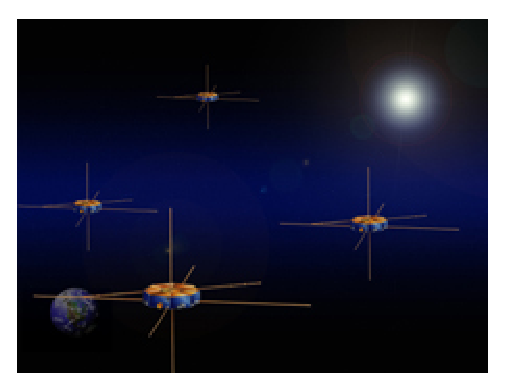
\psfig{file=figures/mms_spacecraft_formation.eps,height=1.2in}}
\caption{MMS Spacecraft Formation}
\label{fig:magneticfields}
\end{figure}

A reconnection event occurs when magnetic field lines cross allowing energetic particles to traverse from interstellar space into the Earth's magnetosphere releasing large quantities of heat and kinetic energy.  The diffusion region of a reconnection event starts on the day side magnetopause an quickly folds over to the Earth's magnetotail (Figure \ref{fig:magneticfields}).  This region is only 1-10 km in size but can travel at 10-100 km/hr \cite{swri} making it extremely difficult to measure.  Effects of a reconnection event are regularly experienced via the aurora borealis, interference with spacecraft GPS systems, and disruptions to electrical grids and communication networks.

\begin{figure}[H]
\centerline{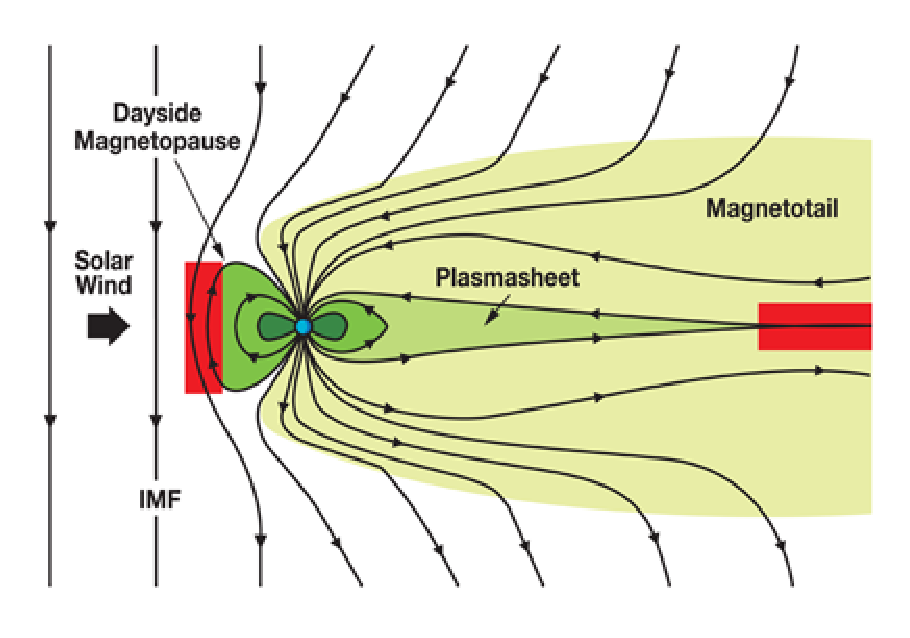
\psfig{file=figures/2d_earth_mag_field_lines.eps,height=1.2in}}
\caption{Earth's magnetic field}
\label{fig:magneticfields}
\end{figure}

Despite the widely experienced effects of reconnection events, very little about the microphysics inside its the diffusion region has been adequately measured.  Magnetometers, spectrometers, and other equipment currently in orbit are only able to capture a small fraction of the event's behavior.  Most equipment collect data from a single point or direction in space or some can get a 360 view of space by applying a slow spin to the spacecraft.  Both of these measurement methods are insufficient at capturing the structure of the diffusion region as it passes.

MMS's four satellites will be equipped with instrumentation mounted at the end of six boom extending out from the spacecraft's body along each major axis.  Four boom are the Spin Plane Double Probes (SDP) and two Axial Double Probes (ADP).  This configuration along with high resolution electron and ion spectrometers gives the constellation a new insight into the internal structure of the diffusion region.  The instrumentation at the ends of the boom are an advantage to the science portion of the mission, but create a unique challenge for the Attitude Determination and Control Systems (ADCS).  The satellites are spin stabilized at a rate of 3 rpm.  Disturbances to the rotation could translate into undesirable boom dynamics and nutations off the spin plane.



% Science questions to answer \cite{mms_website}
%     What determines when reconnection starts and how fast it proceeds?
%     What is the structure of the diffusion region?
%     How do the plasmas and magnetic fields disconnect and reconnect in the diffusion regions?
%     What role do the electrons play in facilitating reconnection?
%     What is the role of turbulence in the reconnection process?
%     How does reconnection lead to the acceleration of particles to high energies?


% \todo{image of formation flight}
% study microphysics of
%   magnetic reconnection
%   energetic particle acceleration
%   turbulence

% s/c MMS-1, MMS-2..MMS-4
% reconnection: Electromagnetic energy from the sun interacts with Earth's magnetosphere causing magnetic field lines to cross and create a burst of energy \cite{nasa_edge_video_ne_at_mms}
% magnetic reconnection measured ions and electrons as boundary passes to create 3d model of it passing by
% Fast plasma investigation
% probing the electron diffusion region (EDR) (passes too rapidly to get an accurate view with current equipment small (1-10 km) and rapidly moving (10-100 km/s))
% adjacent magnetic fields generally have significantly different orientations such that when they intersect, a large amount of energy is dispursed within a small region in the form of heat and kinetic energy.  The region = diffusion region
% explore magnetic reconnection
% dynamic regions of magnetosphere
% orbits planned to pass through the upstream and downstream magnetic reconnection sites
% 1) day side - solar wind field lines connection
% 2) down stream -
% 3) plasma travels down and causes the Arura
% through magnetospheric reconnection, portals allow energetic particles to traverse from outside to the interior of the magnetosphere
% predict when solar space weather within the magnetosphere and if they will affect orbiting satellites
% adverse space weather within the magnetosphere can negatively impact spacecraft system health GPS, induce disruptive current in electrical grids, communications, increased radiation exposure on trans-polar flights

% Difficult to understand
% magnetic boundary passes satellites quickly so has been hard to measure
% MMS has instruments to capture measurements
% Instruments mounted on all sides of the
% 8 sensors 1/30th sec instead of

% October 2014, Atlas five launch \cite{nasa_edge_video}

% Sensors
%   star sensor -> attitude
%   accelerometers -> $\Delta V$


% Fast Plasma Instrument (FPI) - controls
%   16 Dual Electron spectrometer (DES) Goddard built
%   16 Dual Ion Spectrometer (DIS) Japan *** built, hand delivered
%   180 degree and +- 22 degree measurement
%   30 millisec measurement rate 100x faster than previous missions entire view of sky
% FPI
%   despins data

% Instument Data processing Unit (IDPU) - brains of measurements
%   collects, compresses, transmits requested measurement data
%   configure while on mission

% booms
%   eight deployable booms
%   two 12.5m axial booms (electric field sensors)
%   four 60m wire booms
%   two 5m booms in spin plane for magnetometers
% rigid, wire, top/bottom booms
% important to keep consistent spin rate to get accurate estimates of boom location


% \section{Propulsion}

% types: solid propellents, bi propellents, electro propulsion, cold gas systems
% chose: mono-propellant blowdown - hydrozene power thrusters \cite{nasa_edge_video_propulsion}
% 3 rpm
% radial thrusters - spinning
% axial thrusters - prevent nutation

% concern:
% propulsion introduce distrubances

% 20 second pulses

% fuel limits by number of adjustments


% \section{performance requirements}

% $\pm 0.5$ deg attitude tollerance
% 1/10th of a second

\section{Research Objective}
\label{sec:ResearchObjective}

The work described in this thesis utilizes an experimental tabletop satellite (TableSat) \cite{vessthesis} to span three main efforts.  First is to create a physical model of a satellite from NASA's Magnetospheric MultiScale (MMS) Mission in order to validate and compare varied gyroless attitude determination and control (ADC) techniques.  The ADC systems must keep the TableSat rotating at a constant 3 rpm, prevent boom oscillations, and correct for detected nutations off the spin plane.  The second goal is to produce a software system that can be used to run against both theoretical simulations and experimental models.  The third goal is improve TableSat's use as an outreach tool.  The system should provide near ``real-time'' feedback of the system's state, allow for on-the-fly modification to control parameters, and be designed such that a individuals specializing in control systems could customize and extend its functionality without substantial computer science expertise.

\section{Past Work}
\label{sec:PastWork}

This work is a direct extension off of Vess' \cite{vessthesis} research using TableSat through Matlab Simulink and onboard flight controllers to demonstrate fundamentals of control theory.  The TableSat experimental design was modified to study the system dynamics of the instrument booms and nutation actuators in NASA's MMS mission satellites.  Previous experimental \cite{tsat1b} \cite{tsat1c} \cite{tsat2} and analytical \cite{mushawehthesis} ADC work at University of New Hampshire's Advanced Control Lab (ACL) has been done targeting the MMS mission.  The TableSat platform or similar derivations have also been adapted in investigate other areas of research including embedded systems development \cite{tablesat_xuml} and fault tolerant control \cite{tablesat_object_bench} \cite{nanjing_university}.


\section{Analytical and Experimental Testbed}
\label{sec:AnalyticalandExperimentalTestbed}



\section{Thesis Contributions}
\label{sec:ThesisContributions}

This research contributes to the field of feedback control, particularly as it relates to spin stabilized spacecraft, in the following ways:

\begin{itemize}
\item Gyroless observer-based controllers used to detect and eliminate nutations and maintain control of a spin stabilized satellite.
\item Improved capabilities of validating observer-based control methods by keeping identical control systems between analytical simulations and real experiments.
\item Allow clusters of estimators and controllers to all receive the same update for improved side-by-side comparisons of effectiveness.
\item Reduce time required to tune a controller by allowing for gain adjustments and swapping of estimation/control techniques on-the-fly.
\item Decompose quaternion state into separate rotational and nutation quaternions for use in error correction.
\item Use decomposed quaternion and differentiated rotational quaternions to decouple rate and attitude control.
\item Base quaternion state corrections on the representative rotational angle error, not the quaternion's sinusoidal scalar term.
\item Build the application such that the same control laws can be used to drive analytical simulations as well as experimental tests with physical systems.
\item Develop the application in a modular fashion to easily allow for future improvements and additions.
\item Control rates between modules such as sensors to estimators and estimators to controllers are independent and can operate at separate rates.
\item ``run-time'' feedback is available to visualize how the controller believes the system is responding.
\item A global clock instance is used for the authoritative time which during simulations can be adjusted in runtime to speed up or slow down the simulation to obtain better insight into the system dynamics.
\item Compensations for variable step sizes ($\delta t$) are made where able to protect the numerical integrity of the controller under large changes in control rates.
\item Code covered by proper software unit tests to validate and maintain expected behavior of the system during software upgrades.
\item Provide the combination of ``run-time'' visualizations and on-the-fly parameter/controller tuning for outreach programs.
\item Write the control application in a high level language to keep it accessible for improvements to control systems engineers with moderate programming experience.
\end{itemize}

\section{Thesis Outline}
\label{sec:ThesisOutline}




\chapter{UNH TableSat 1A}
\label{chap:UNHTableSat1A}

The UNH TableSat 1A is a limited 3-DOF experimental test bed analog for the NASA MMS satellite (See Figure \ref{fig:TSatFullView}).  All electronics, booms, and actuators are attached to a circular PVC deck.  The aluminum hub at its center has a hollow center which allow it to rest on a center post giving the deck full rotation about its z-axis and limited rotations about its x and y-axes.  Five out of the six booms present on the MMS spacecraft are represented on TableSat 1A.  The four SDP booms extend radially from the deck at 90 degree intervals.  One of the MMS's ADP booms is modeled with a boom attached to the center post of the TableSat.



\begin{figure}[H]
\centerline{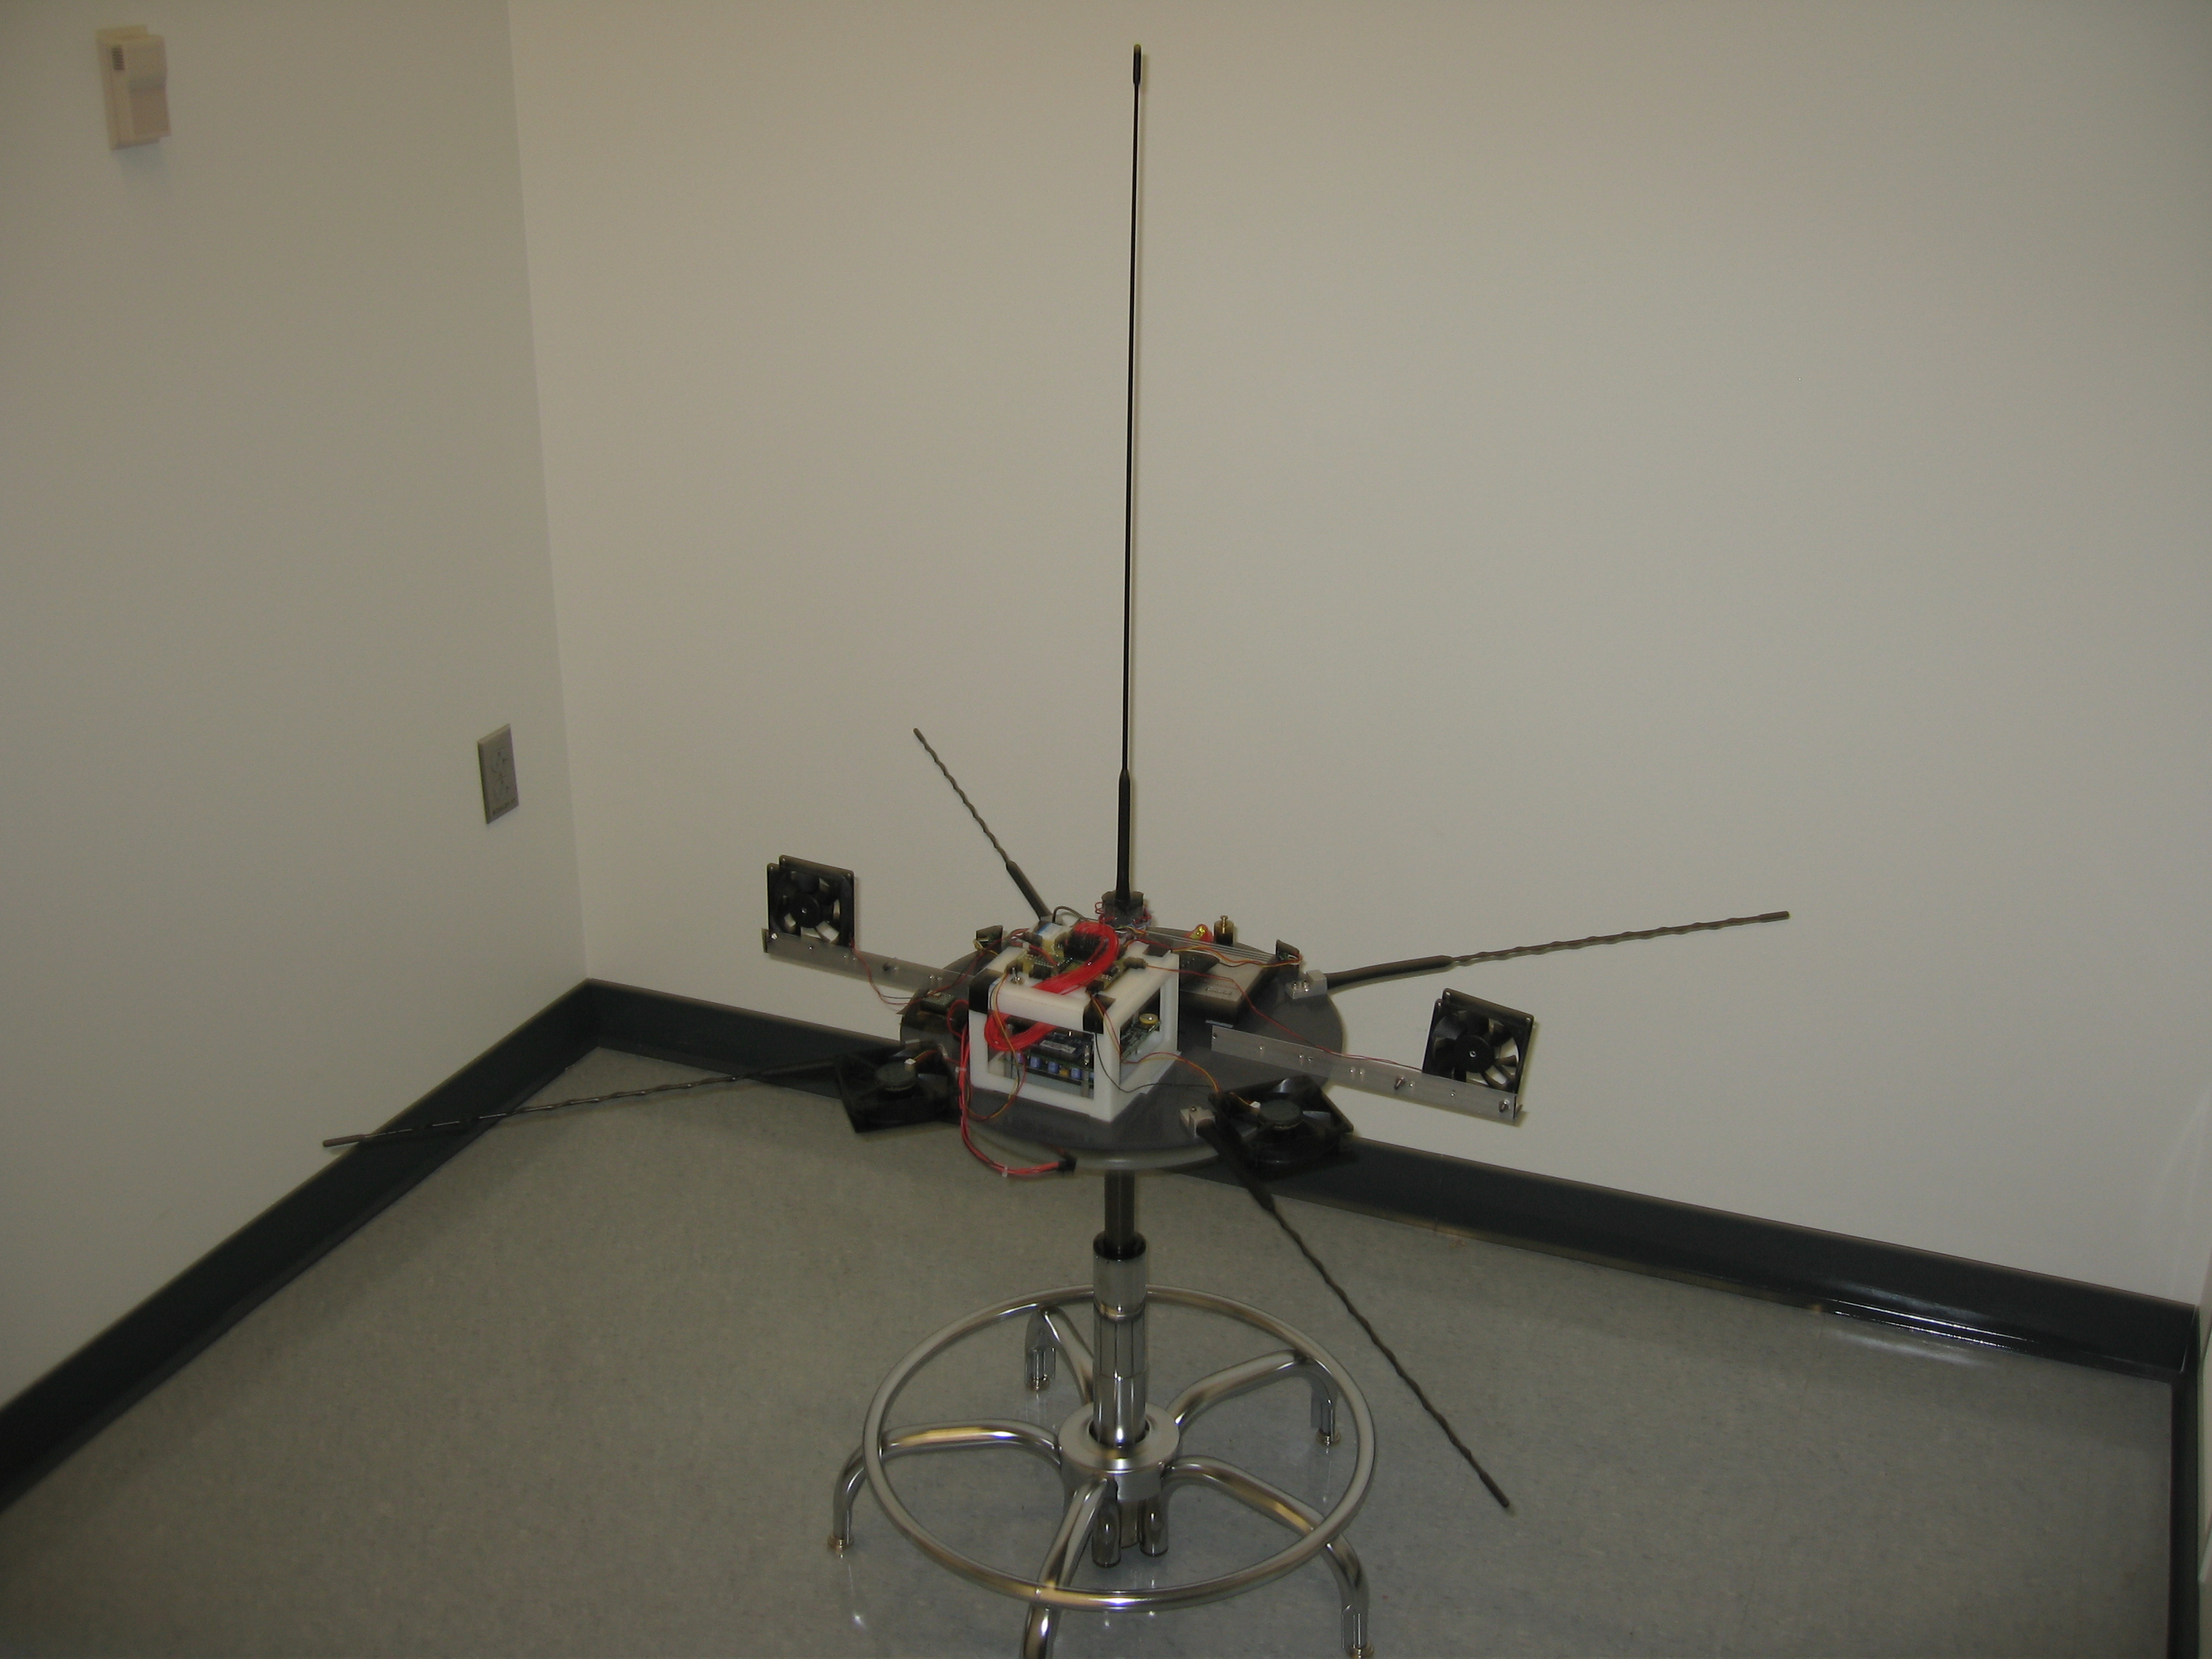
\psfig{file=figures/tsat_full_view.eps,height=3in}}
\caption{TableSat 1A Full View}
\label{fig:TSatFullView}
\end{figure}

\section{Booms}
\label{sec:Booms}

The ADP booms were modeled with a selection of flexible antenna.  Attaching weights to the tip and varying the stiffness of the selected antenna allowed for some tuning to the fundamental frequency of the booms.  Since the SDP booms extend perpendicularly to gravity, two choices were made for their modeling.  For free motion, the cylindrical antenna for the ADP boom were also used for the SDP booms.  The disadvantage to these booms especially when adding weights to reduce their natural frequency was that they would droop under the gravitational pull.  An alternative to the cylindrical antenna for the SPD booms were thin and flat strips of metal.  Attaching them to the TableSat's deck such that they were standing on edge removed the gravitational drooping since the booms, but still allowed for the boom to bend back and forth in the spin plane.  This also restricted the boom's freedom of movement, so a combination of results would be needed to get a better idea of how the MMS booms would react in orbit.

\begin{figure}[H]
\centerline{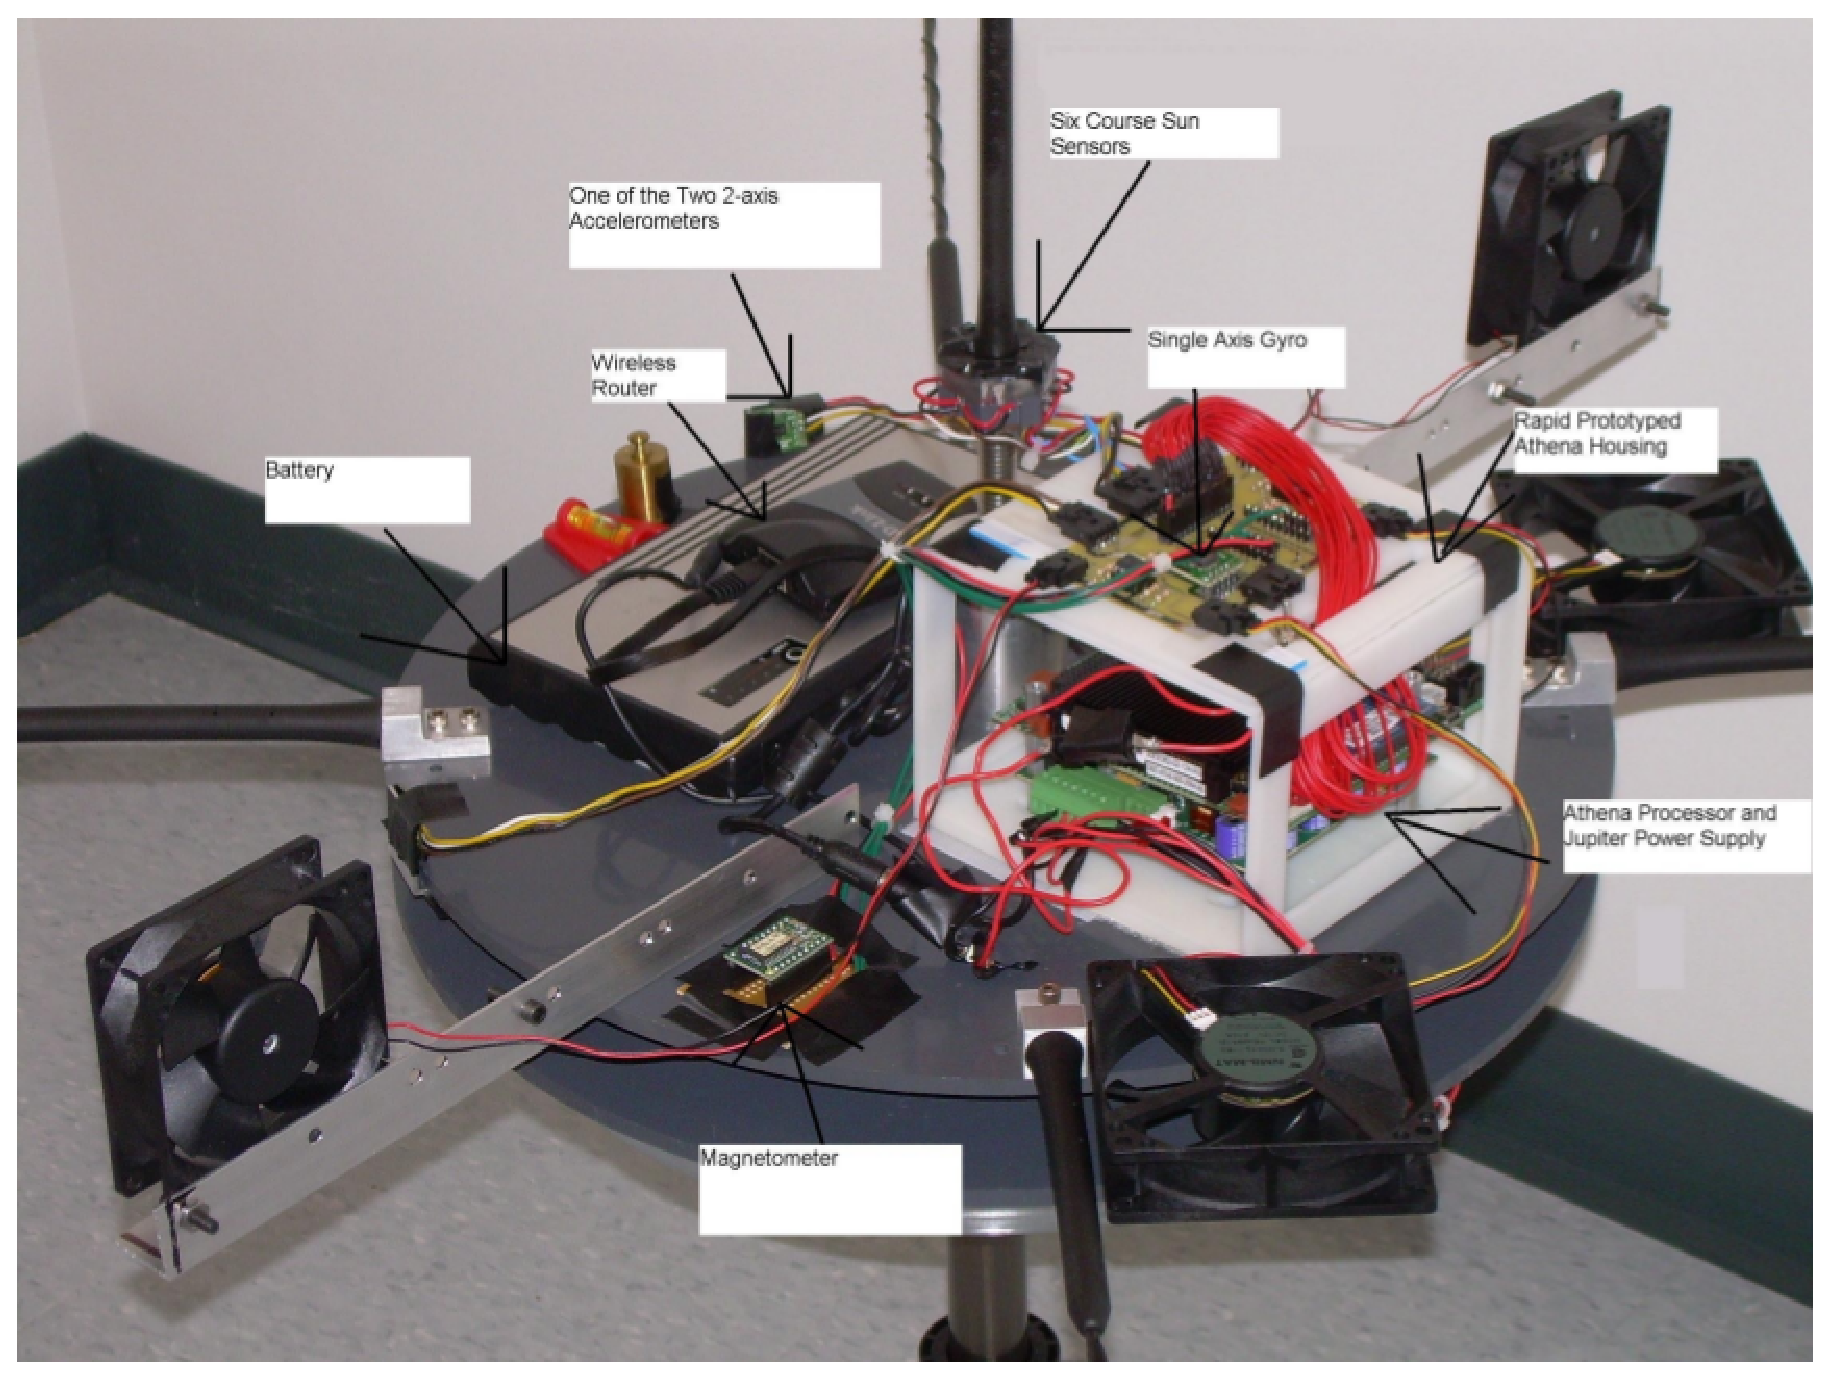
\psfig{file=figures/tsat_components.eps,height=4in}}
\caption{TableSat Components}
\label{fig:TSatComponents}
\end{figure}

\section{Flight Controller}
\label{sec:FlightController}

The onboard flight controller was an Athena PC from Diamond Systems powered by a Jupiter power supply and lithium-ion rechargeable battery.  The Athena processor and Jupiter power supply were mounted in a rapid prototyping housing with open sides for ventilation.  A custom printed circuit board designed by Jeff Kite \TODO{need footnote reference here?} was mounted on top of the rapid prototyping housing.  User Datagram Protocol (UDP) communication (Section \ref{subsec:MessageDefinitions}) to the base station is transmitted through a wireless access point.

\TODO{forgot cs student's name} created a C program based off of Vess' ``open-loop'' flight controller \cite{vessthesis} .  This program is responsible for listening to a UDP socket on the TableSat and performing a limited set of actions based on the message packets received from the base station.  The most common messages triggered actions like altering the voltages applied to the actuators, and scanning the sensor ports and sending the voltages back to the base station through UDP.

\section{Actuators}
\label{sec:Actuators}

In addition to the booms extending from the TableSat's deck, four single direction analog input computer fans were mounted to provide a source of thrust (Figure \ref{fig:TSatComponents}).  Two fans were mounted standing upright to provide radial torque.  One pointing clockwise and the other counter clockwise had their centers level with the pivot point inside the central hub and provided control of the rotation rate.  Two other fans were mounted facing down to provide limited opportunities for nutation control.

\section{Sensors}
\label{sec:Sensors}

Four classes of analog sensors were implemented in TableSat 1A's design. Gyroscope (Section \ref{subsec:Gyroscope}) and accelerometer (Section \ref{subsec:Accelerometer}) for velocity measurements.  Course sun sensor (Section \ref{subsec:CourseSunSensor}), and magnetometer (Section \ref{subsec:TripleAxisMagnetometer}) for position measurements.  These sensors and the four actuators filled all available analog ports on the onboard Athena flight computer.  As is described below, the gyroscopes and accelerometers were not used for the observer-based controllers in this thesis leaving just positional measurements from the course sun sensors and triple axis magnetometer.

\begin{figure}[H]
\centerline{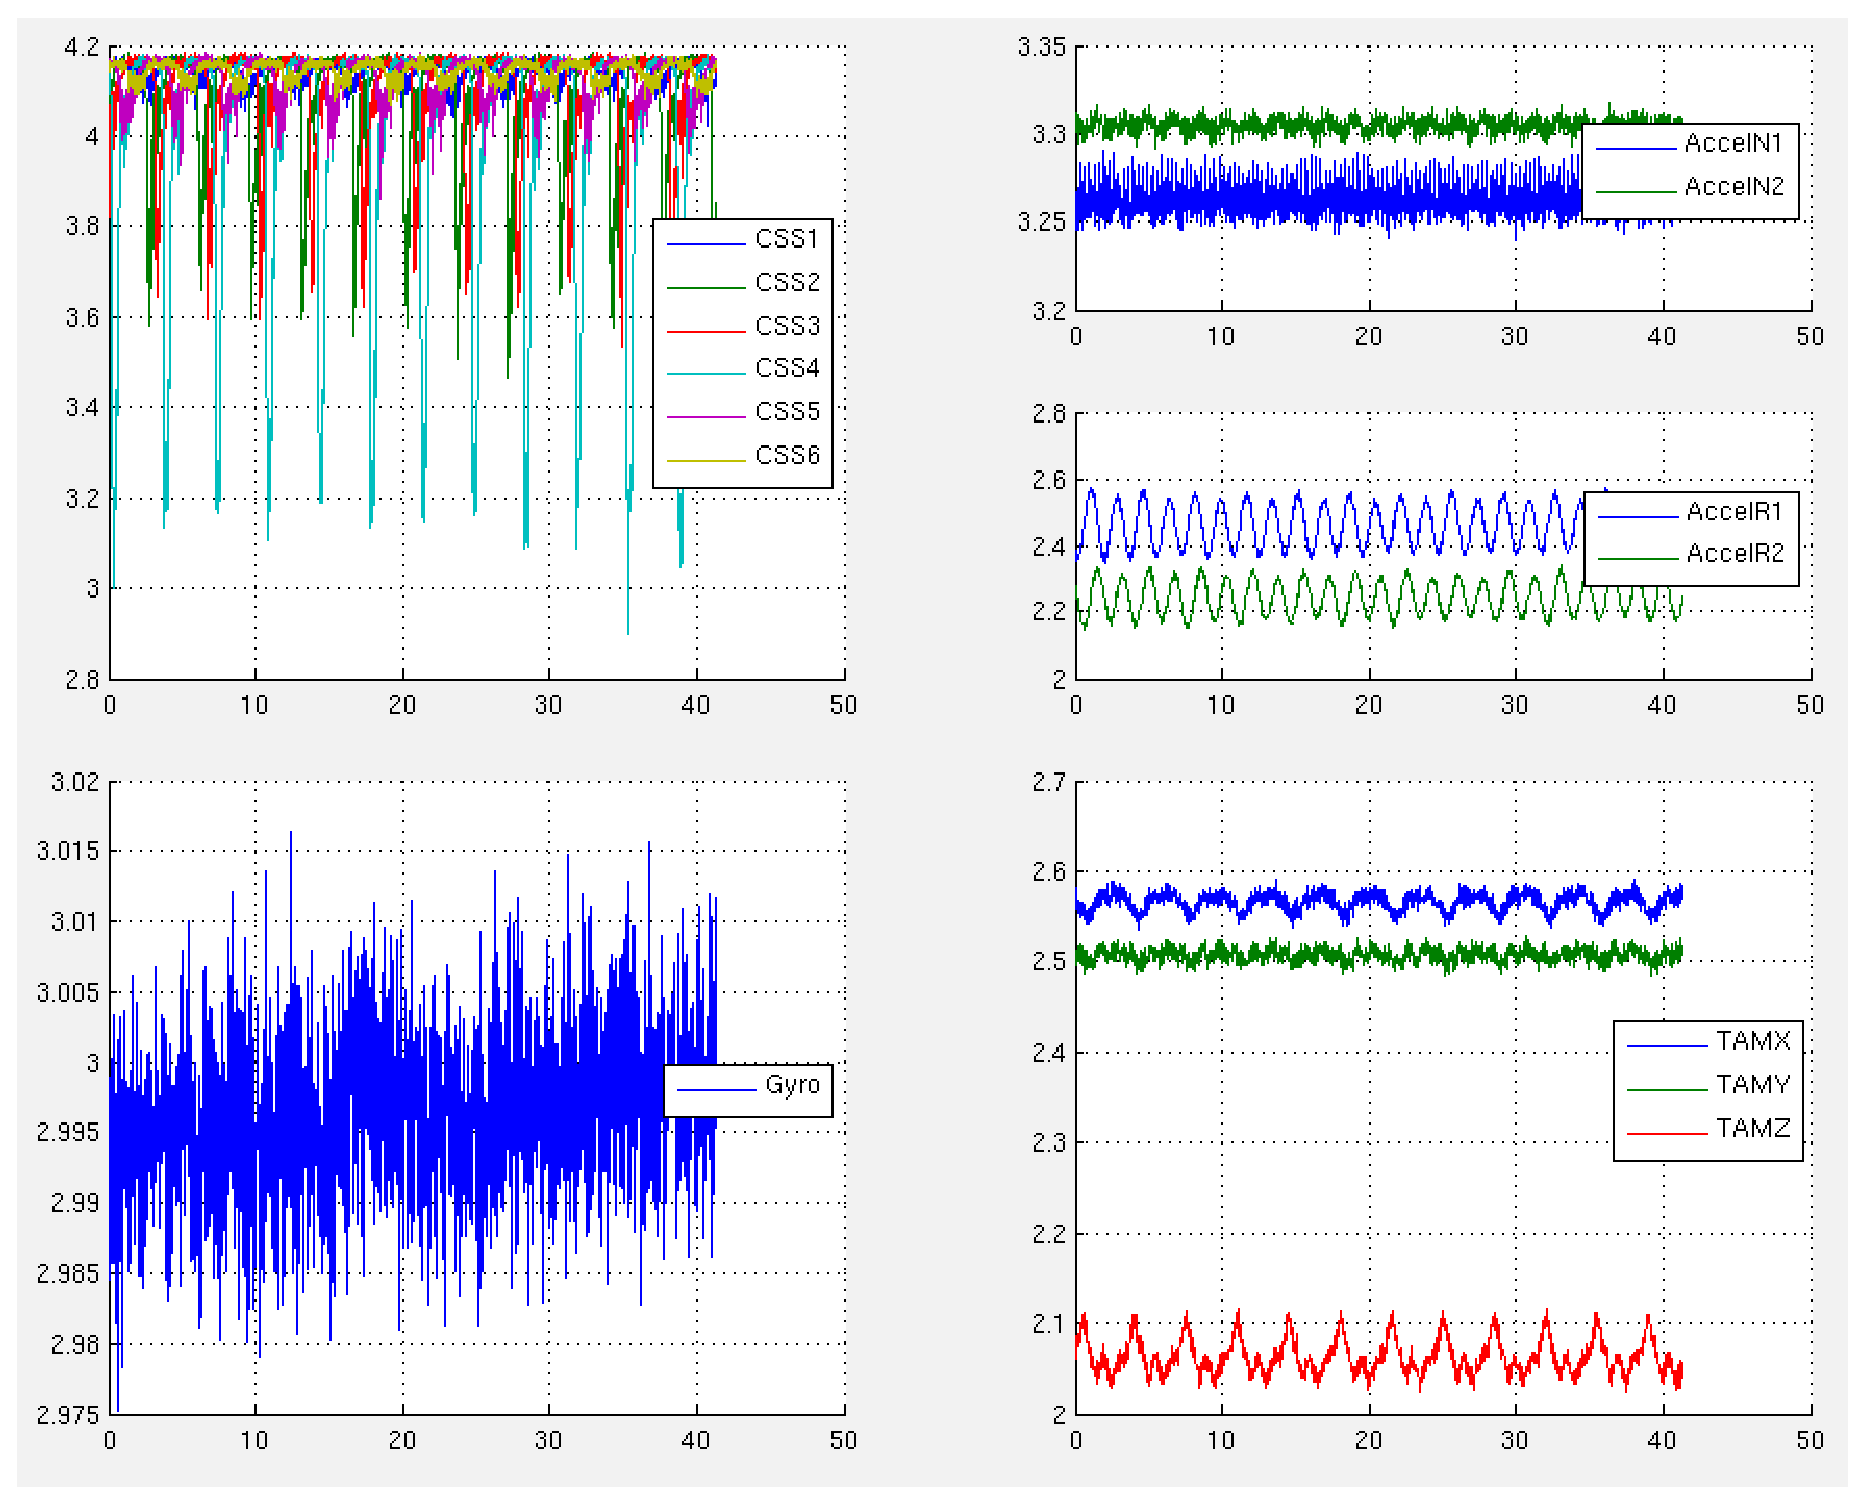
\psfig{file=figures/sensor_voltage_charts.eps,height=4in}}
\caption{Sensor Voltage Readings}
\label{fig:SensorVoltageReadings}
\end{figure}

\subsection{Gyroscope}
\label{subsec:Gyroscope}

Gyroscopes remain one of the most accurate sensors for detecting changes to a structure's angular body rates.  The issue with their use is that to increasing the accuracy of a gyroscope means using a heavier sensor.  Since any additional weight is a serious launch concern for a satellite, this research for NASA's MMS mission uses the gyro scope solely as a verification method.  The gyroscope selected for TableSat 1A is a single axis gyroscope that is mounted on the printed circuit board at the top of the flight controller housing.  The gyroscope is oriented to detect changes in body rates about the TableSat's z-axis although is mounted slightly above the center hub's pivot point so will pick up small signals from any limited nutation encountered.

\subsection{Accelerometer}
\label{subsec:Accelerometer}

Two 2-axis accelerometers are mounted at the circumference or TableSat's deck.  The accelerometers are oriented such that one signal detects vertical acceleration with a 2g resolution and the other a radial signal with a 0.5g resolution.  The rotational accelerometers ended up picking up a small signal which is either due to oscillations in angular velocity or a nutation subjecting the radial accelerometer to gravitational effects.  The vertical components of the accelerometers had such low signal to noise ratios that heavy filtering would be required to even attempt to detect the out of plane rotations.  Any significant nutations allowed by the limited 3-DOF design would damp out quickly enough to be eliminated before the filtering could identify the signal.  Given these severe limitations in the sensor's measurements, for the purpose of this thesis the accelerometer measurements are ignored.

\subsection{Course Sun Sensor}
\label{subsec:CourseSunSensor}

The course sun sensor (CSS) for UNH TableSat 1A was constructed from a hexagonal piece of PVC pipe with a photodiode mounted in each face (Figure \ref{fig:CSS}).  Photodiodes are light detectors that convert captured light to electricity.  Given the inability to use the gyroscope and the accelerometer's high level of noise, the course sun sensor proved to be the most reliable sensor, but was limited to measuring a single value from the state matrix corresponding to rotations about the z-axis.  Each photo diode detected light level in its field of view and would generate a voltage generally proportional to that value.  The photodiodes are mounted above the center hub and faced out around the spin plane.  By placing a single light source in a dark room, the course sun sensor's voltages could be used to calculate the angular displacement about the body's z-axis.


\begin{figure}[H]
\centerline{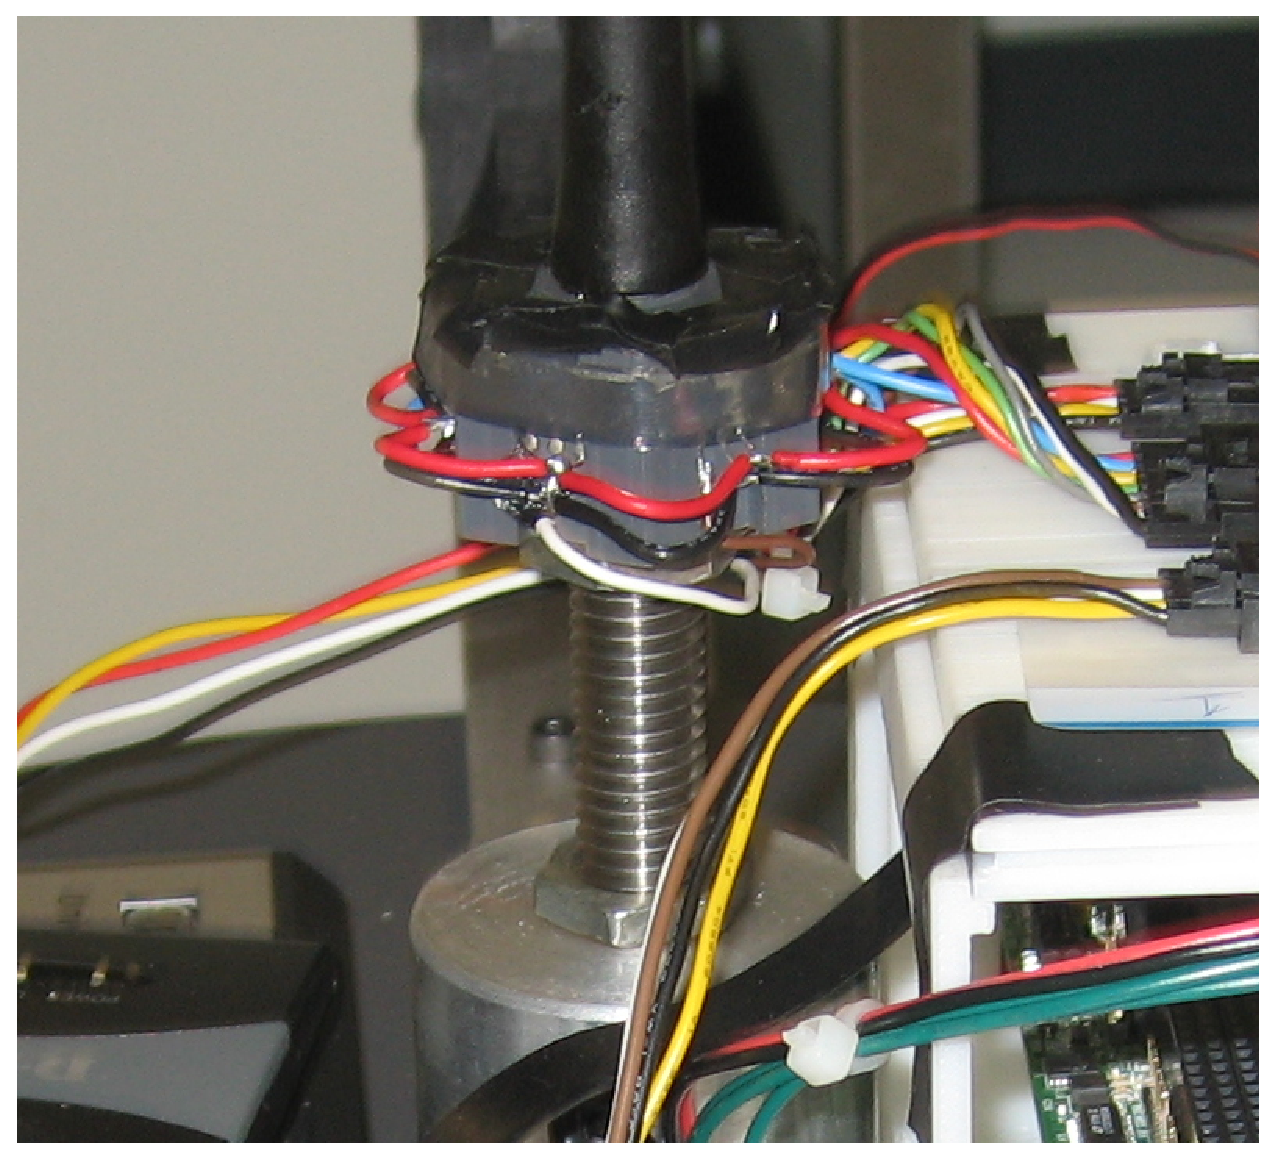
\psfig{file=figures/css.eps,height=2in}}
\caption{Course Sun Sensor Configuration}
\label{fig:CSS}
\end{figure}

Calculating the angular displacement about the body's z-axis is done using a method similar to a resultant force calculation.  Assuming all of the photodiodes volts per lumen rates are consistent, the voltages can be described as an equivalent force it the direction of the photodiode face.  Each force is decomposed into x and y components and then summed into a resultant force vector who's angle is used to represent the angular displacement of the TableSat.  Even though this method is fairly simplistic and that individual sensor voltage readings contained a moderate level of noise, this method proved to generate a very reliable and clean signal before even using filtering and estimation techniques.

\begin{subequations}
  \begin{align}
    V_{css\_x} & = \sum\limits_{i=1}^6 (V_{css\_x} - V_{css\_base}) \cos \left( \frac{2\pi}{6} (i-1)\right) \\
    V_{css\_y} & = \sum\limits_{i=1}^6 (V_{css\_x} - V_{css\_base}) \sin \left( \frac{2\pi}{6} (i-1)\right) \\
    \psi & = \tan^{-1} \frac{V_{css\_y}}{V_{css\_x}}
  \end{align}
  \label{eqn:CSSResultantForce}
\end{subequations}

\begin{figure}[H]
\centerline{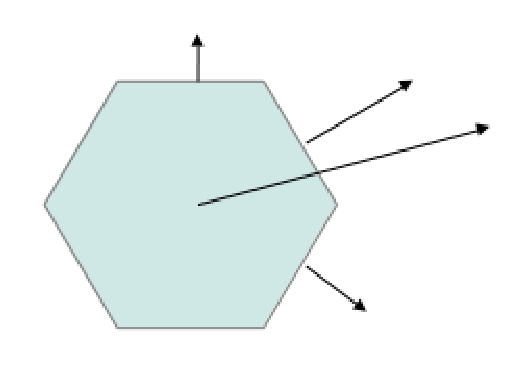
\psfig{file=figures/css_vectors.eps,height=1in}}
\caption{Photodiode Resultant Force Calculation for Yaw}
\label{fig:CSSVectors}
\end{figure}


\subsection{Triple Axis Magnetometer}
\label{subsec:TripleAxisMagnetometer}

Along with the course sun sensor, the triple-axis magnetometer (TAM) is used to measure position.  The primary advantage to the TAM over the course sun sensor it that it measures the full position state rather than just position about the z-axis.  As seen in Figure \ref{fig:SensorVoltageReadings}, three voltages are reported to designate the TableSat's attitude.  Each voltage corresponds to the strength of the magnetic field in each orthogonal direction.  To determine a method of converting raw TAM voltages to a TableSat, the clockwise actuator was set to provide a constant thrust.  With the fraction of the pivot point, the system slowly stabilized to a relatively constant spin rate.  Once stabilized, TAM voltage readings were recorded at a rate of 50 Hz and written to a log.  The mean values were subtracted from each of the three axes and plotted (Figure \ref{fig:TAMRaw}).

\begin{figure}[H]
\centerline{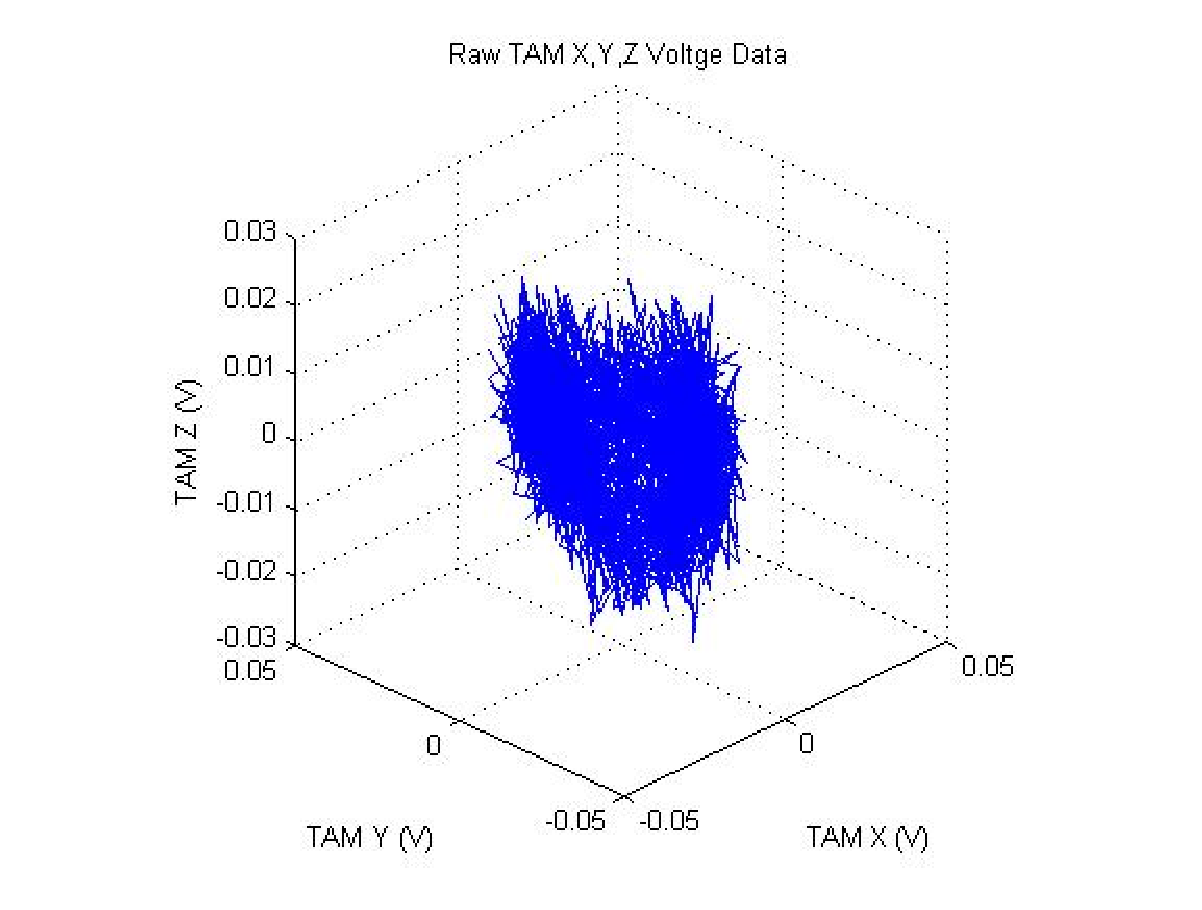
\psfig{file=figures/tam_raw.eps,height=4in}}
\caption{Raw TAM Voltages}
\label{fig:TAMRaw}
\end{figure}

Besides the slightly less dense center, the raw TAM measurements amount to a blob of points with no clear pattern.  If the signal is strong enough, a consistent path should be present.  Given the high sampling rate, aggressive filtering should be able to pull a signal out of the blob of data points.  A basic 40 point moving average was used as a first pass analysis to verify there is a signal in the data (Eq \ref{eqn:TAMMovingAvg}).  The moving average smoothed data is show in Figure \ref{fig:TAMMovingAverage}.  The good news being that a distinct an repeatable signal occurs as TableSat completes successive rotations.  The bad news is the irregular path that the magnetometer readings follow.

\begin{equation}
  x_i = \frac{1}{40} \sum^{39}_{j=0} x_{i-j}
  \label{eqn:TAMMovingAvg}
\end{equation}

\begin{figure}
  \begin{subfigure}[h!]{0.5\textwidth}
    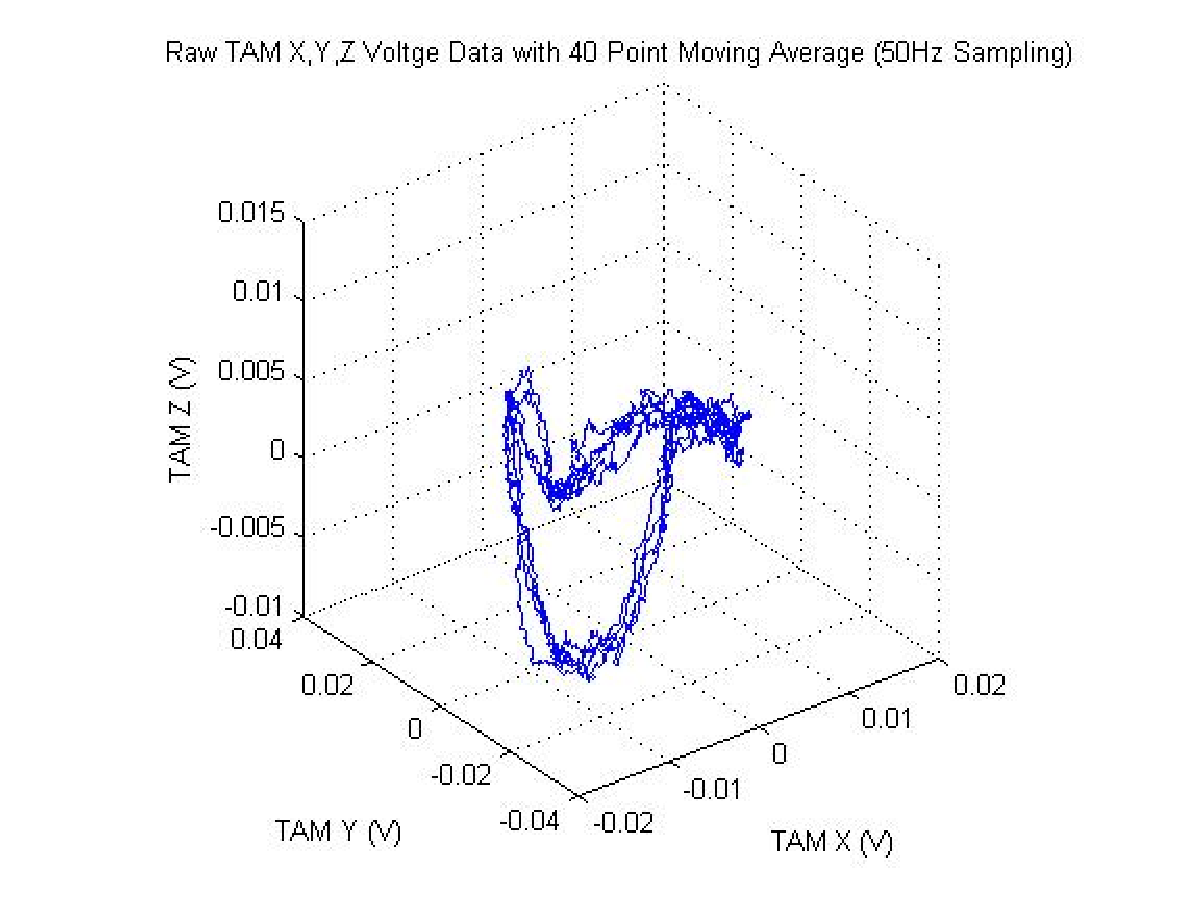
\includegraphics[width=\textwidth]{figures/tam_moving_average.eps}
    \caption{Raw TAM Voltages - Moving Average}
    \label{fig:TAMMovingAverage}
  \end{subfigure}
  ~
  \begin{subfigure}[h!]{0.5\textwidth}
    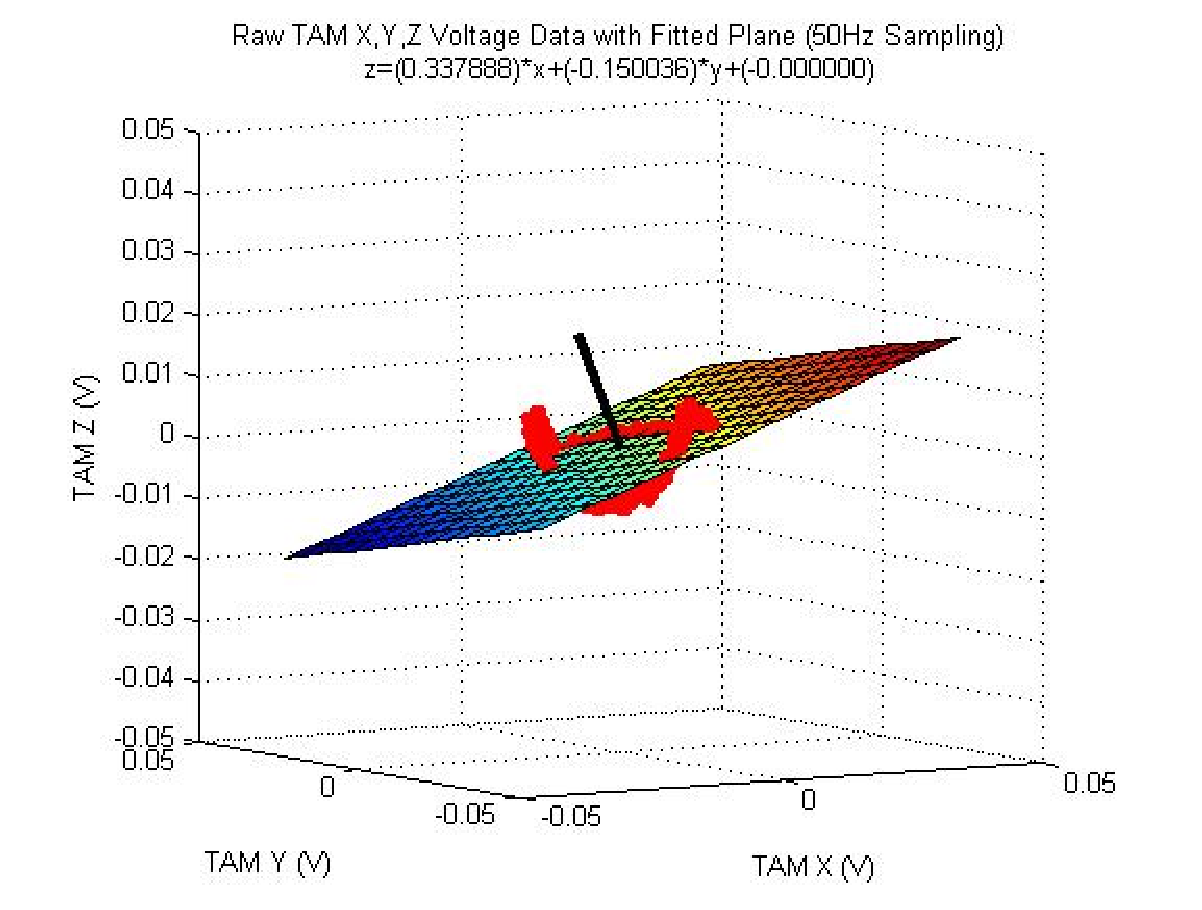
\includegraphics[width=\textwidth]{figures/tam_fitted_plane.eps}
    \caption{TAM Voltages with Fitted Plane}
    \label{fig:TAMFittedPlane}
  \end{subfigure}
  \caption{Determining Attitude from TAM}
  \label{fig:TAMSignal}
\end{figure}

Figure \ref{fig:TAMFittedPlane} shows the result of fitting a plane to the moving average smoothed TAM voltages.  The error in the fit between the smoothed TAM data points and the planar fit were too large to have much confidence in using this measure for nutation detection.

Following this analysis, the magnetic field surrounding the experimental setup was tested.  Moving a compass through the test space showed large swings in magnetic field lines despite the setup being placed on a wooden table in the middle of the lab.  Subsequent sweeps of the lab located a space with a relatively uniform magnetic field.  A uniform thrust was applied to the clockwise actuator and voltages logged as before.  Performing the moving average smoothing provided verification of the expected behavior of the magnetometer (Fig \ref{fig:TAMUniformField})

\begin{figure}[H]
  \centerline{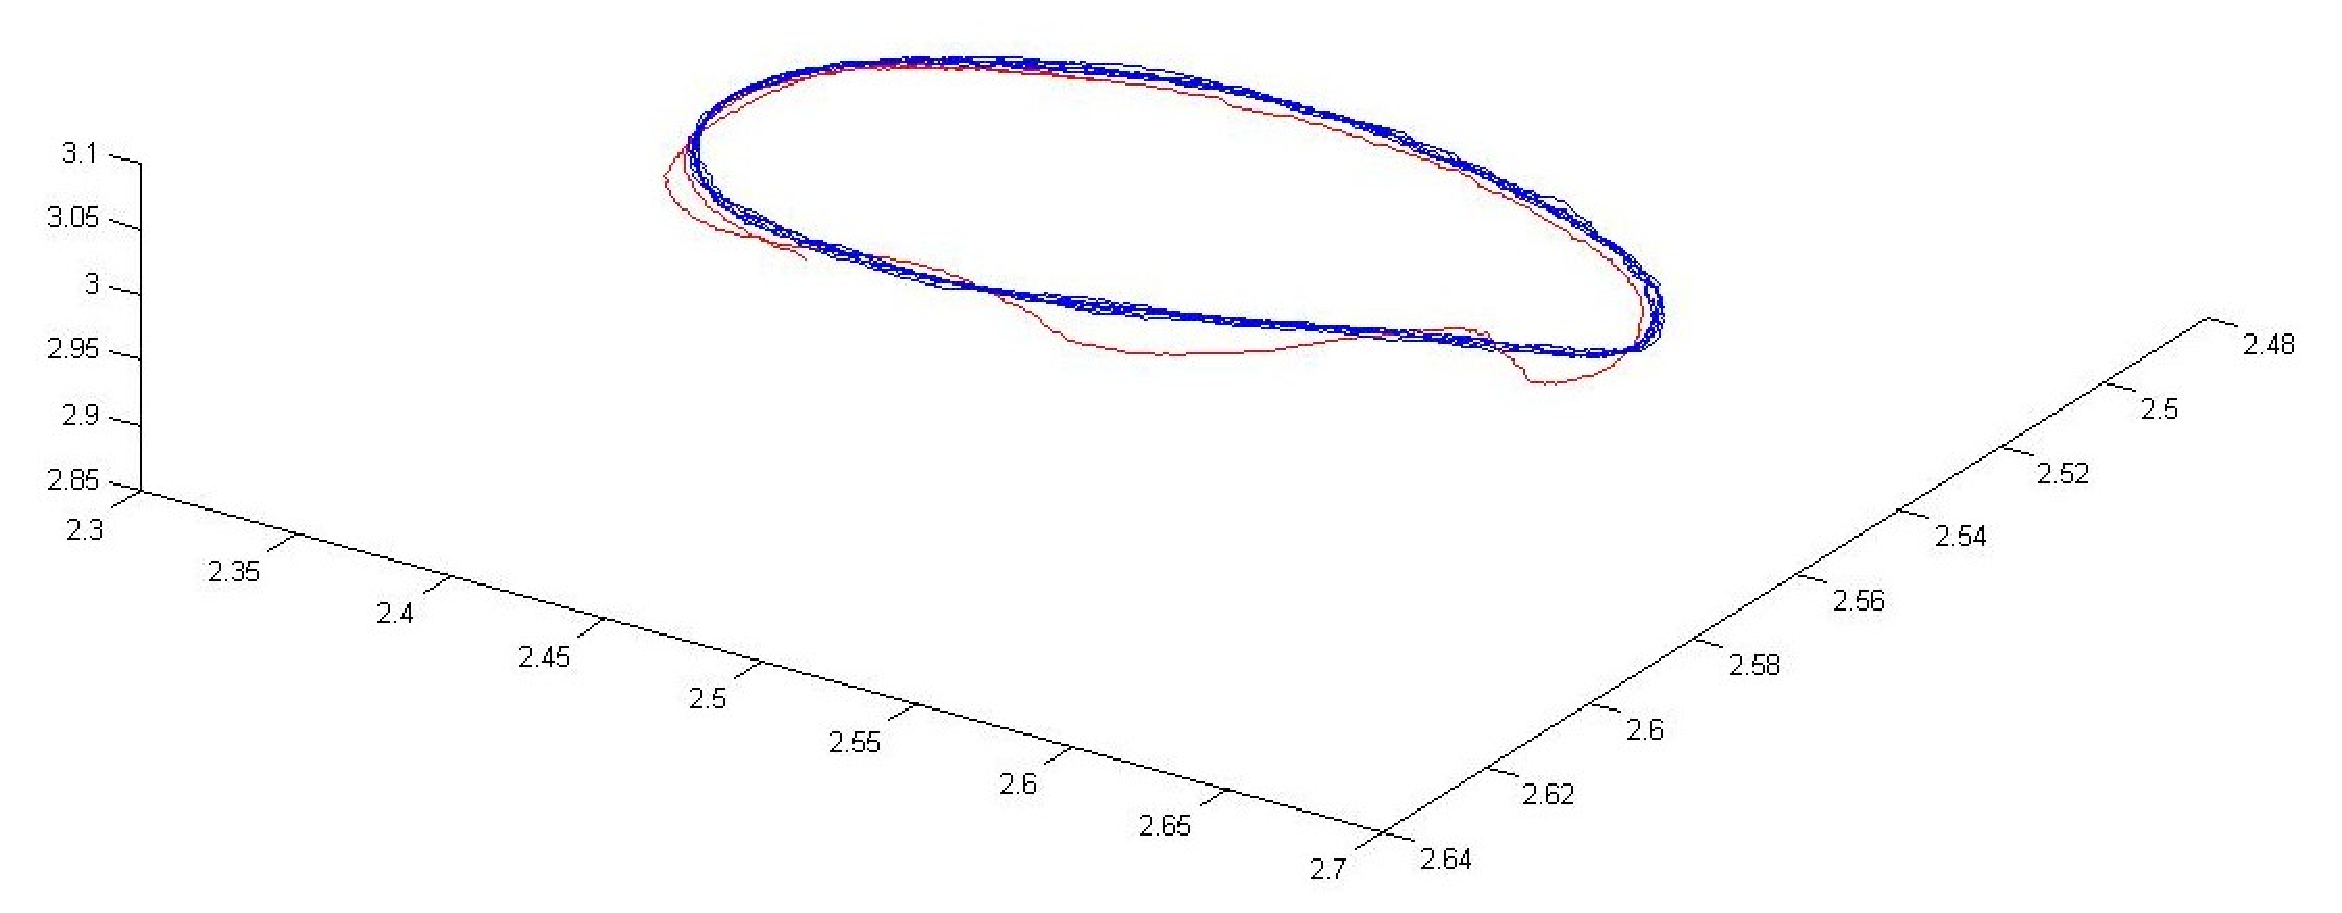
\psfig{file=figures/tam_uniform_field.eps,width=0.8\textwidth}}
  \caption{TAM measurements in a uniform field}
  \label{fig:TAMUniformField}
\end{figure}

Since the gyroscope and accelerometers were determined to be useless for the observer based controller, and the course sun sensors only able to detect motion about the z-axis, the triple-axis magnetometer remained the only sensor onboard that had the capability of detecting the nutation required for the MMS controller.

The baseline path established for TableSat in the absence of nutation (Fig fig:TAMUniformField) should be able to be compared to readings during a live run of the system and any offsets used to quantify nutation.  The same process of rotating the TableSat under a constant thrust was repeated four more times.  Each time a 200g brass weight was placed on the TableSat's deck at each principle axis $+x, +y, -x, -y$ causing the TableSat to pivot about 14 degrees out of the spin plane which was about the extent its range for nutation.  The TAM voltages for each run are grouped by color and shown in Figure \ref{fig:TAMNutationVoltages}.  Although the paths intersect and measurements are not $1:1$ to the TableSat's orientation, there is at least a separation in paths.  Further study found that while the TAM voltages are duplicated between nutation paths, points that occupy the same space in the TAM measurement have different yaw measurements as measured by the course sun sensor.

\begin{figure}[H]
  \centerline{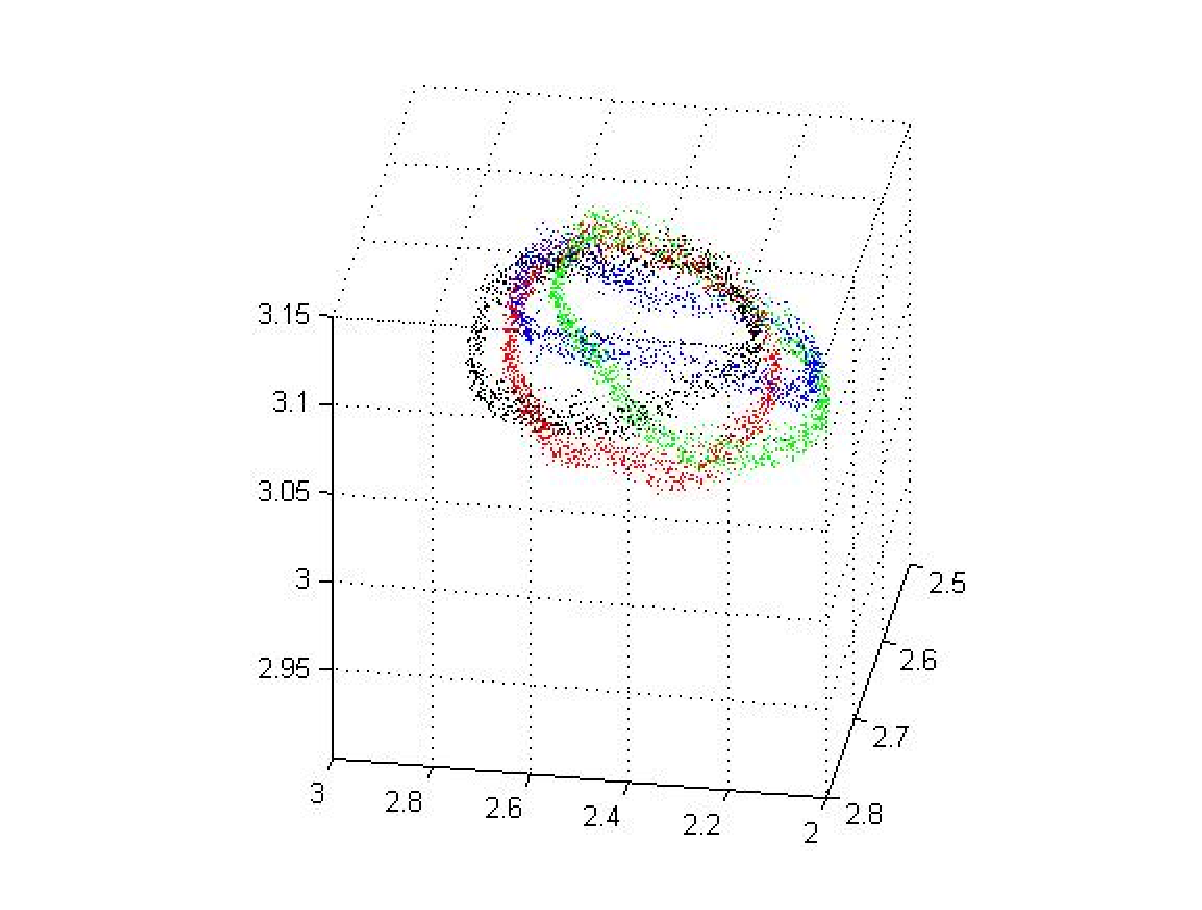
\psfig{file=figures/tam_distinct_tilts_with_good_field.eps,height=4in}}
  \caption{TAM nutation voltages}
  \label{fig:TAMNutationVoltages}
\end{figure}

\section{TableSat State Measurement}
\label{subsec:StateMeasurement}

As covered in the sections above, the only sensors available for state measurement of TableSat 1A for the observer based controller were the course sun sensor and the triple axis magnetometer.  Both of which individually measure a portion of the system's attitude and leave the system's body rate unmeasured.

Combining the measurements of the course sun sensor and triple axis magnetometer provided high confidence in the yaw measurement and rough estimates about the roll and pitch nutations.  An algorithm was developed that started with the course sun sensor and through equation \ref{eqn:CSSResultantForce} produced a measurement of yaw.  The TAM calibration data was synthesized to create a reference table of TAM readings at each of the five paths (steady, and the four nutations shown in Figure \ref{fig:TAMNutationVoltages}).  This reference table along with the equation to determine yaw from the course sun sensor are comined through a method descibed in \ref{subsec:SampleAttitudeCalculation} to approximate the TableSat's attitude.

\begin{table}[H]
  \centering
  \begin{tabular}{c|ccc|ccc}
    \hline
    Yaw   & & Steady & & & $+X \ 14^o$ & \\ \hline
    (deg) & $TAM_x$ (V) & $TAM_y$ (V) & $TAM_x$ (V) & $TAM_x$ (V) & $TAM_y$ (V) & $TAM_x$ (V)  \\ \hline
    0 & $S_{x0}$ & $S_{y0}$ & $S_{z0}$ & $+X_{x0}$ & $+X_{y0}$ & $+X_{z0}$ \\ \hline
    1 & $S_{x1}$ & $S_{y1}$ & $S_{z1}$ & $+X_{x1}$ & $+X_{y1}$ & $+X_{z1}$ \\ \hline
    ... & & & & & &  \\ \hline
    Yaw   & & $+Y \ 14^o$ & & & $-X \ 14^o$ & \\ \hline
    (deg) & $TAM_x$ (V) & $TAM_y$ (V) & $TAM_x$ (V) & $TAM_x$ (V) & $TAM_y$ (V) & $TAM_x$ (V)  \\ \hline
    0 & $+Y_{x0}$ & $+Y_{y0}$ & $+Y_{z0}$ & $-X_{x0}$ & $-X_{y0}$ & $-X_{z0}$ \\ \hline
    1 & $+Y_{x1}$ & $+Y_{y1}$ & $+Y_{z1}$ & $-X_{x1}$ & $-X_{y1}$ & $-X_{z1}$ \\ \hline
    ... & & & & & &  \\ \hline
    Yaw   & & $-Y \ 14^o$ & &  \\ \hline
    (deg) & $TAM_x$ (V) & $TAM_y$ (V) & $TAM_x$ (V)  \\ \hline
    0 & $-Y_{x0}$ & $-Y_{y0}$ & $-Y_{z0}$  \\ \hline
    1 & $-Y_{x1}$ & $-Y_{y1}$ & $-Y_{z1}$  \\ \hline
    ... & & & & & &  \\ \hline
  \end{tabular}
  \caption{TAM calibration reference table}
  \label{tbl:TAMCalibration}
\end{table}

\subsection{Sample Attitude Calculation}
\label{subsec:SampleAttitudeCalculation}

This example will go through a sample calculation of the nutation based on a single set of course sun sensor and triple axis magnetometer voltage measurements.

\subsubsection{Scan Sensor Voltages}

The base station submits message id 20 to TableSat which responds with a message 63 with a payload containing 15 floats (timestamp, 6 photodiodes, 4 accelerometrs, gyroscope, and 3 triple-axis magnetometer).

\subsubsection{Calculate Yaw From Course Sun Sensor}

Using sample CSS voltages from the photodiodes of 0.37247, 0.30899, 1.18370, 2.40020, 1.80500, and 0.44052.  The TSatPy python package whose development is detailed in Chapter \ref{chap:TSatPy} uses equation \ref{eqn:CSSResultantForce} to convert the sensor voltages into a meaningful state.

\begin{singlespace}
  \begin{minted}[mathescape,
               linenos,
               numbersep=10pt,
               frame=lines,
               framesep=2mm]{python}
import TSatPy
import numpy as np

css_v = [0.37247, 0.30899, 1.18370, 2.40020, 1.80500, 0.44052]

pda = TSatPy.Sensor.PhotoDiodeArray()
pda.update_state(css_v)
vector, radians = pda.x.q.to_rotation()

print "A %g radian (%d degree) rotation about <%g, %g, %g>" % (
    radians, radians / np.pi * 180,
    vector[0,0], vector[1,0], vector[2,0])

# Prints out
# A 3.34585 radian (191 degree) rotation about <-0, -0, -1>
  \end{minted}
  % \nocite{minted}
\end{singlespace}

\subsubsection{Create Calibration TAM Data}

About 1020 data points per calibration set
Average of 37 data points per degree




\section{Messages Between TableSat and the Base Station}


\subsection{Message Protocol}
\label{subsec:UDPTCP}

Communication between the controller and the experimental TableSat is negotiated over a User Datagram Protocol (UDP) socket.  Both the controller and TableSat read and write over port 9877.  UDP is used for a stateless connection more generally used for pushing data over a large number of connections.  The other common communication protocol is Transmission Control Protocol (TCP) where a session is established between server and client and successful transferral of data is acknowledged by the recipient.

Advantages and disadvantages exist between the TCP and UDP protocols and became a critical factor in influencing the design of TableSat 1A base station controller. Section \ref{sec:Simulink} goes into further detail in how this difference in protocols cropped up early in the development of the base station controller where the combination of Matlab Simulink with a UDP communication protocol produced a very fragile system.

A UDP message transmission is done in a ``fire and forget'' fashion.  The message header can generally include the originating hosts ip address and port so that the server knows where to send the response.  The session-less nature of UDP means that the originating server sends the message, but does not receive confirmation that the message transmitted successfully as with TCP where ever interaction is followed up with an acknowledgment from the other host.

The advantage to using UDP for the UNH TableSat 1 is that the satellite side code could be largely based off of Melissa Vess' work on her TableSat thesis where the control loop was implemented on-board, and the UDP connection was used to infrequently poll for data or modify sensor calibration values.  The UDP connection has the slight advantage of being able to transmit and receive packets without needing to wait for acknowledgments.  This could save a small fraction of time, but on modern hardware and with the small bandwidth usage this advantage is negligible.

Disadvantages to a UDP implementing the control interface through UDP include the possibility of packet loss where the sender submits a packet, but it gets corrupted or dropped.  Since UDP is a stateless connection, the sender doesn't wait for an acknowledgment which in this case would not come. This issue is handled by the communications module.  If the control loop rate on both updating the actuator voltages and polling sensor data is fast enough, a dropped packet would not matter much since a new updated set of values would be soon to follow.  Issues could be caused if the completion of a code loop was dependent on a packet coming in.  If dropped, the control loop could block until the next packet is received.  This was one issue encountered in the project version [sec:ControlLoopinSimulink].


\subsection{Message Definitions}
\label{subsec:MessageDefinitions}


The packet structure used for this project is the same as used by Melissa Vess \cite{vessthesis}. Each UDP packet is comprised of a packet header and data payload.  The packet header format remains constant for all messages containing five octets of data.

\begin{table}[H]
  \centering
  \begin{tabular}{| l | l |}
    \hline
    Header Octet & Description \\ \hline
    h1 & Message Number (0 to 255) \\ \hline
    h2 & Flags (0 - 255) \\ \hline
    h3 & Message Size (0 - 255) \\ \hline
    h4 & Message Size (0 - 255) \\ \hline
    h5 & 0 \\ \hline
  \end{tabular}
  \caption{UDP message headers}
  \label{tbl:UDPMessageHeaders}
\end{table}

The first octet (h1) contains the message number that matches to a predefined list of messages known by both the sender and recipient.  This is used to specify how the data in the payload is to be used.

The second octet (h2) is reserved for flags.  For some messages, flags can be set for additional data.  These are not used in the final implementation of UNH TableSat 1A.

The third (h3) and fourth (h4) header octets define the size of the data's payload, so when reading data in from a buffer, the header can inform the recipient how many bytes need to get read in from the buffer in order to get to the end of the packet.  For payloads less than 256 bytes only the fourth header byte is needed.  For payloads larger than 255 bytes the following formula is used to specify the message size headers.

\begin{subequations}
  \begin{align}
    h4 &= mod(size, 256) \\
    h3 &= floor(size / 256)
  \end{align}
  \label{eqn:UDPSizeHeader}
\end{subequations}

The only meta data provided along with the payload beyond the data's size is an 8 bit message number.  Both UNH TableSat 1A and the control station have identical message list definitions.

\begin{table}[H]
  \centering
  \begin{tabular}{|l|l|l|l|}
    \hline
    Message Id & Payload Size & Data Type & Message Description \\ \hline
    2 & 1 octet & unsigned int & Set run mode \\ \hline
    4 & 1 octet & unsigned int & Set run mode \\ \hline
    18 & 4 x (8 octets) & float & Set fan speed \\ \hline
    19 & 1 octet & unsigned int & Set log record mode \\ \hline
    20 & 1 octet & unsigned int & Request sensor reading \\ \hline
    22 & 1 octet & unsigned int & End of sensor log \\ \hline
    23 & 8 octets & float & Request sensor log data \\ \hline
    33 & 8 octets & float & Set log sample rate \\ \hline
    63 & 15 x (8 octets) & float & Sensor readings \\ \hline
    64 & 16 x (8 octets) & float & Sensor log entry \\ \hline
    65 & 8 octets & float & Sensor log size \\ \hline
    104 & 1 octet & unsigned int & Ack run mode \\ \hline
    118 & 1 octet & unsigned int & Ack fan volt \\ \hline
    119 & 1 octet & unsigned int & Ack sensor log run mode \\ \hline
    133 & 1 octet & unsigned int & Ack log sample rate \\ \hline
  \end{tabular}
  \caption{TableSat message definitions}
  \label{tbl:UDPMessageDefinitions}
\end{table}


\chapter{Analytical}
\label{chap:Analytical}

\section{Standard Observer Based Controls Cruft}
\label{sec:StandardObserverBasedControlsCruft}

\section{Simulation Results}
\label{sec:SimulationResults}




\chapter{STANDARD CONTROL THEORY TOOLS}
\label{chap:StandardTools}

\section{Simulink}
\label{sec:Simulink}

Slight variation of the ``open loop'' control system used in part of Melissa Vess' TableSat research.  Huge problem with fault tolerance.  The format chosen for relaying messages resulted in an unreliable exchange of data between the base station (laptop) and the TableSat.  These error were compounded with Matlab Simulink's inability to handle the unexpected lack of message data.

\TODO{More detail here on the Simulink side.  Specify pros of this design.  Include screen shot of simulink diagram for a P controller.}


\section{TSat Message Center}
\label{sec:TSatMessageCenter}

This was the first full rework of the control system.  The focus of this design was to eliminate the use of Matlab Simulink diagrams, and directly control the messages transmitted and received.

\TODO{Elaborate on the failures of the design.  Inability to handle two tasks at one.  State persistence.  No visualization.  }



\chapter{SOFTWARE DEVELOPMENT FOR EXPERIMENTAL INTEGRATION}
\label{chap:SoftwareDevelopmentforExperimentalIntegration}

\TODO{Finish this}

\section{Runtime Control and Analysis}
\label{sec:RuntimeControlandAnalysis}

\TODO{Finish this}

\section{Object Oriented Matlab Control System}
\label{sec:ObjectOrientedMatlabControlSystem}

\TODO{Finish this}

\chapter{TSatPy}
\label{chap:TSatPy}

Chapter \ref{chap:ProgressionOfControlSystemSoftware} detailed the progression through the initial four versions of the attitude determination and control system (ADCS) that are written in or for a Numerical Simulation Software (NSS) implementation.  While these versions provide a level of insight and control into a control system, the NSS environment is not a natural fit for that level of programming and presents issues that take a significant effort to work around.  On top of some of the issues with diagnosing problems, the NSS controller code targets a fairly narrow swath of professions that are comfortable with using and editing it.  Because of this, the final version was written in Python, a common cross-platform and open source programming language.

Python is quoted as coming ``batteries included'' which is a statement to the number of common libraries that come standard with the language including a \verb|socket| library for sending and receiving User Datagram Protocol (UDP) packets used by TableSat.  Python is also known as an expressive language where what a section of code does is generally easily discernible from a quick read.

To support the control system written for this thesis being easily available for others to use and edit, python includes a variety of unit test frameworks for ensuring consistency, and gives the ability to write self-documenting code.  Self-documenting code means that if have an instance of a class stored in a variable \verb|v| but are unsure what can be done with the class, typing \verb|help(v)| will print out documentation about the various methods available and how they are used.

Section (\ref{sec:KeyCharacteristics}) covers some of the notable characteristics about the TSatPy implementation of the ADCS, and Section (\ref{sec:Module Design}) describes the different types of classes that are written for the program and what their role is.

\section{Key Characteristics}
\label{sec:KeyCharacteristics}

\subsection{Adaptive Step Algorithms}

All time dependent calculations vary their parameters at run-time dependent on the time since the last time it ran. For example, the integral component of a PID controller with an error measure of $+0.2$ will accumulate an error of $+0.02$ for the first $\Delta t_k = 0.1$ sec, but will only accumulate an additional $+0.016$ for the next time step of $\Delta t_{k+1} = 0.08$ sec.  This functionality avoids the errors encountered when a system is linearized about an assumed time step, but the actual time step varies which causes the controller gain values to be over or under aggressive.

\subsection{Variable System Clock}

The system clock is the official time keeper for the entire ADCS. Advantages to using a central clock instead of the computer time is that the rate of elapsed time can be modified at run-time during simulations to either compress the time to complete the simulation or slow down the simulation to inspect a transient event. (See Section \ref{subsec:IntegralEstimator})

\subsection{Quaternion Multiplicative Corrections}

Quaternions that quantify a system's position contain 4 values that through common control systems implementations are tracked and controlled separately. This approach ignores the restriction that rotational quaternions maintain a unit norm while the adjustments are made then scale the resulting quaternion back to a unit norm compromising the predictability and stability of the control system.  Using the object oriented programming to track the scalar and vector components ensures that controllers can be built that make use of the quaternion multiplicative correction technique which maintains the integrity of the values and their relation to the physical attitude of the system. (See Section \ref{subsec:QuaternionAttitude})

\subsection{Theta Multiplier with Quaternion Vector Balancing}

Unlike body rates that can be linearly scaled, the 4 quaternion values are sinusoidal values where multiple values can represent the same attitude (i.e. 0, 360 degrees). Scaling the sinusoidal values directly produces inconsistent adjustment rates. All quaternion scaling in the TSatPy software is performed against angle that the quaternion represents. With this method, we can maintain the linear scaling affect that is desired while maintaining the integrity of the quaternion representation. (See Section \ref{subsec:ThetaMultiplierWithQuaternionVectorBalancing})

\subsection{Run-time interface}

Through the use of a python twisted daemon process an restful API interface is available to query the state of the system in the middle of a run. This creates the ability to display meaningful representations of the system and increase insight into the system's dynamic behavior instead of relying on batch post processing.  This functionality is built into the last NSS version of the software, but has not yet been ported over to the python code base. (See Section \ref{sec:ObjectOrientedNSSControlSystem})

\subsection{Concurrent Estimation/Control Algorithms}

When running a comparative analysis between different types of estimators or different types of controllers, common methods are to re-run simulations for each variation and compare the results. The library allows for configurations such as providing the same measurement values to both a PID and SMO estimator to compare their performance. (See Section \ref{sec:ComparativeAnalysysofPIDandSMOEstimators})

\subsection{Quaternion Decomposition}

With spin-stabilized satellites, five degrees of freedom are available to compare against a fixed desired value.  The quaternion decomposition method allows the separation of the yaw motion from the remained of the attitude representation enabling the 5-DOF control of constant body rates and removing nutation. (See Section \ref{subsec:SpinStabilizedControl})

\subsection{Modular Design}

This library is designed to have interchangeable components with predefined and consistent interfaces and roles by allowing for the inclusion of additional estimation and control techniques. In the case of estimation, an Extended Kalman Filter (EKF) class can be added by creating a new class in Estimator.py that has contains the common properties ($\bs{\hat{x}}$, $\bs{x}_e$..) and common methods ($\bs{\hat{x}}$ = update($\bs{x}$)).

\subsection{Portable Design}

The portable design dictates that with the defined interfaces between modules, the observer based control methods have no knowledge of what is producing the sensor readings and what is accepting moment commands. This enforces consistency in the behavior of the system whether it's hooked up to an in-memory model of a satellite, NASA MMS TableSat 1A, or any future spin spin-stabilized platform.

\subsection{Python}

There can be a disconnect between the control systems engineer that regularly complete their design and analytical work in a Numerical Simulation Software environment (like Matlab Simulink or Octave) and the software engineer who implementation the control method in a more standard language. By using a language like python, the code can be written in an expressive manner so that a control systems professional only needs a little programming experience to modify the code. It also keeps the controller in a language than could be reviewed for optimization by a software engineer and applied directly to the experimental platform without requiring a conversion to an entirely different system or language.


\section{Module Design}
\label{sec:Module Design}

Below is an outline of the separate modules contained in the TSatPy library and their associated roles.

\subsection{Actuators}
\label{subsec:actuators}

input: Desired moment\\
output: Actual moment\\

This module defines the output of the controller. The actuator instance on initialization, is supplied with the physical arrangement of the actuators. During run-time the actuator module first accept a $\Re^3$ moment from the controller.  It then compares what it's being asked to do with what can actually be supplied.  That true moment is then available for use with estimator state propagation, and for conversion to actuator voltages. (See Section \ref{sec:ActuatorConfiguration})

\subsection{ADCS}
\label{subsec:ADCS}

input: Configuration file\\
output: ADCS model\\

This module is intended as the main parent object.  As an input it will read a json configuration file that defines all the components and parameters required for a specific observer-based controller.


\subsection{Clock}
\label{subsec:Clock}

input: None\\
output: Elapsed time\\

This module establishes the authoritative source for elapsed time and is continually referenced by any time-dependent logic such as integral or derivative based parameters. The metronome class by default track seconds since the initialization of the clock, but when running simulations can have it's speed dynamically altered to either run faster for long term simulations or run slower to get better inspection of an event.


\subsection{Comm}
\label{subsec:Comm}

From Controller to Satellite\\
input: Voltage setting determined by the actuator\\
output: UDP packet to the system or in-memory model\\
From Satellite to Controller\\
input: Sensor voltages from the system or in-memory model\\
output: Sensor data to submit to sensor class for conversion to a state\\

This module handles the interface between the the control system and either the physical system or the theoretical model. With the physical system, a UDP socket is opened and either listens for packets transmitted from the sensors or submits voltage packets to set actuator voltages. When running in simulations, the module submits and receives the voltage messages to an in-memory model of the system that contains the system dynamics and can return mocked sensor voltages based on the behavior.


\subsection{Controller}
\label{subsec:Controller}

input: Estimated state ($\bs{\hat{x}}$)\\
output: Moment couples ($\bs{M}$)\\

This module contains the algorithms that compare the estimated system behavior with the desired behavior and determine what moments required to make the system behave as desired.

The master controller instance governs the interface between the incoming estimator state and the outgoing actuator moments. The master controller can run multiple control algorithms simultaneously which can be individually tuned to different types of system behaviors like one that can handle large errors and one for the soft corrections at steady state.


\subsection{Estimator}
\label{subsec:Estimator}

input: Measured state ($\bs{x}$)\\
output: Estimated state ($\bs{\hat{x}}$)\\

This module contains the algorithm that take the measured state from the sensor model which is likely based on noisy sensor data and attempts to attenuate the effects of the noise to create an accurate representation of the true state of the system.

\subsection{Sensor}
\label{subsec:Sensor}

input: Voltages ($\bs{V}$)\\
output: Measured state ($\bs{x}$)\\

This module receives raw voltage measurements from either a simulated truth model of the system or from the Comm module polling sensor voltage data off the experimental TableSat.  Each class represents a different sensor type (coarse sun sensor, magnetometer, gyroscope, ...) and contain the logic to convert sensor readings from that sensor into a state representation $x$ with quaternion and body rates.


\subsection{Service}
\label{subsec:Service}

input: Run configuration\\
output: Twisted daemon\\

Coupled with the ADCS module the Service module is intended to create the daemon that manages the interactions between all the modules including sockets to TableSat.


\subsection{StateOperator}
\label{subsec:StateOperator}

input: An instance from the State module\\
output: A modified State instance or the conversion to a new State instance\\

This module contains classes that are designed to modify instances from the State module such as \verb|BodyRate| or \verb|Quaternion| or convert between them. For example an error quaternion can be scaled up or down by the QuaternionGain class.

\begin{table}[H]
  \centering
  \begin{tabular}{l|p{0.5\linewidth}}
    Class &  What it does \\ \hline
    BodyRateGain & Scale a BodyRate instance\\
    QuaternionGain & Scale a Quaternion instance\\
    StateGain &  Scale the State instance (Wrapper for QuaternionGain, BodyRateGain)\\
    QuaternionSaturation & Saturate a Quaternion\\
    BodyRateSaturation & Saturate a BodyRate\\
    StateSaturation  & Saturate a State (Wrapper for QuaternionSaturation, BodyRateSaturation)\\
    BodyRateToMoment & Convert a BodyRate to a Moment\\
    QuaternionToMoment & Convert a Quaternion to a Moment\\
    StateToMoment  & Convert a State to a Moment (Wrapper for QuaternionToMoment, BodyRateToMoment)\\
  \end{tabular}
  \caption{State Operators}
  \label{tbl:StateOperators}
\end{table}



\subsection{State}
\label{subsec:State}

This module contains classes that are used to quantify the state of the system.

\begin{table}[H]
  \centering
  \begin{tabular}{l|p{0.5\linewidth}}
State  & Class \\ \hline
Quaternion & Attitude \\
BodyRate & Body-fixed angular velocities \\
QuaternionError & Difference in attitudes \\
QuaternionDynamics & How body rates change the attitude \\
EulerMomentEquations & How moments change the body rates  \\
State & Position and velocity \\
StateError & Differences in position and velocity \\
Plant & In-memory model of the satellite \\
Moment & Applied torques \\
  \end{tabular}
  \caption{State Measurements}
  \label{tbl:State}
\end{table}


\chapter{CONCLUSIONS}
\label{chap:Conclusions}

The goal of this thesis was to determine the viability of the TableSat 1A's platform for comparison and experimental verification of various observer-based controllers.

\TODO{Finish this}

Estimator:
  SMO bettor for initial response
  Toss up between SMO/PID for ss response, SMO update state sooner, PID less error

Controller:
  SMC performs far better with perfect estimates

State Error
  Multiplicative quaternion corrections
  Scaling based or the represented angle rather than the quaternion scalar
  Estimating the vector quantities of the quaternion can interfere with the angular component, only control the use of the angular component (fewer parameters to tune)

Python so much better than matlab for programming
Slow progress to establish the foundation, but became faster as building blocks were created and vetted through unit tests

run-time feedback ++

Attitude control
  Surprising level of control with just a single gain in a P-controller!!!


Antipodal response with P-attitude and body rate control

Quaternion decomposition Equation \ref{eqn:DecomposeQuaternion}
\chapter{FUTURE WORK}
\label{chap:FutureWork}

\TODO{Finish this}

Types of actuators

Actuator PWM

Magnetometer



\begin{thebibliography}{XxxxNN}                 %
                                                %
  \bibitem[Hans80]{FirstRef} D. E. Hanson.      % You need one of these for
      {\em The Title of His/Her Book.}          % each citation.  Use an
      Some Publisher Name,                      % \include{mybib} instead
      Some Big City                             % if you'd rather to keep
                                                % these in a separate file.
  \bibitem[Lamp86]{The-Manual} L. Lamport.      %
      {\em LaTeX, User's Guide \& Reference     % See the manual to find out
      Manual}                                   % why we had to use a backslash
      Addison-Wesley Publish Company            % character (\) in front of the
      Reading, Massachusetts                    % ampersand (&).
                                                %

  \bibitem[Abra90]{abrahams} Abrahams, Paul W.,
    Karl Berry, and Kathryn A. Hargreaves.
    {\em \TeX\ for the Impatient}.
    Addison-Wesley Publishing Company,
    Reading MA, USA, 1990.


  \bibitem[Thom92]{thomas} Thomas, George B. Jr.,
    and Ross L. Finney.
    {\em Calculus and Analytic Geometry},
    8$^{th}$\ ed.
    Addison-Wesley Publishing Company,
    Reading MA, USA, 1992.

\end{thebibliography}

\appendix
  \begin{singlespace}
  % 
\chapter{TSatPy SOURCE CODE}
\label{chap:tsatpy_source}

\linespread{1}

\pagebreak
\section*{TSatPy/ADCS.py}\label{code:TSatPy/ADCS.py}\inputminted[linenos,fontsize=\scriptsize]{python}{/home/dcouture/git/mathyourlife/TSatPy/TSatPy/ADCS.py}

\pagebreak
\section*{TSatPy/Actuator.py}\label{code:TSatPy/Actuator.py}\inputminted[linenos,fontsize=\scriptsize]{python}{/home/dcouture/git/mathyourlife/TSatPy/TSatPy/Actuator.py}

\pagebreak
\section*{TSatPy/Clock.py}\label{code:TSatPy/Clock.py}\inputminted[linenos,fontsize=\scriptsize]{python}{/home/dcouture/git/mathyourlife/TSatPy/TSatPy/Clock.py}

\pagebreak
\section*{TSatPy/Comm.py}\label{code:TSatPy/Comm.py}\inputminted[linenos,fontsize=\scriptsize]{python}{/home/dcouture/git/mathyourlife/TSatPy/TSatPy/Comm.py}

\pagebreak
\section*{TSatPy/Controller.py}\label{code:TSatPy/Controller.py}\inputminted[linenos,fontsize=\scriptsize]{python}{/home/dcouture/git/mathyourlife/TSatPy/TSatPy/Controller.py}

\pagebreak
\section*{TSatPy/Estimator.py}\label{code:TSatPy/Estimator.py}\inputminted[linenos,fontsize=\scriptsize]{python}{/home/dcouture/git/mathyourlife/TSatPy/TSatPy/Estimator.py}

\pagebreak
\section*{TSatPy/Sensor.py}\label{code:TSatPy/Sensor.py}\inputminted[linenos,fontsize=\scriptsize]{python}{/home/dcouture/git/mathyourlife/TSatPy/TSatPy/Sensor.py}

\pagebreak
\section*{TSatPy/Server.py}\label{code:TSatPy/Server.py}\inputminted[linenos,fontsize=\scriptsize]{python}{/home/dcouture/git/mathyourlife/TSatPy/TSatPy/Server.py}

\pagebreak
\section*{TSatPy/Service.py}\label{code:TSatPy/Service.py}\inputminted[linenos,fontsize=\scriptsize]{python}{/home/dcouture/git/mathyourlife/TSatPy/TSatPy/Service.py}

\pagebreak
\section*{TSatPy/State.py}\label{code:TSatPy/State.py}\inputminted[linenos,fontsize=\scriptsize]{python}{/home/dcouture/git/mathyourlife/TSatPy/TSatPy/State.py}

\pagebreak
\section*{TSatPy/StateOperator.py}\label{code:TSatPy/StateOperator.py}\inputminted[linenos,fontsize=\scriptsize]{python}{/home/dcouture/git/mathyourlife/TSatPy/TSatPy/StateOperator.py}

\pagebreak
\section*{TSatPy/\_\_init\_\_.py}\label{code:TSatPy/__init__.py}\inputminted[linenos,fontsize=\scriptsize]{python}{/home/dcouture/git/mathyourlife/TSatPy/TSatPy/__init__.py}

\pagebreak
\section*{TSatPy/tests/Clock\_test.py}\label{code:TSatPy/tests/Clock_test.py}
\inputminted[linenos,fontsize=\scriptsize]{python}{/home/dcouture/git/mathyourlife/TSatPy/TSatPy/tests/Clock_test.py}

\pagebreak
\section*{TSatPy/tests/Controller\_test.py}\label{code:TSatPy/tests/Controller_test.py}
\inputminted[linenos,fontsize=\scriptsize]{python}{/home/dcouture/git/mathyourlife/TSatPy/TSatPy/tests/Controller_test.py}

\pagebreak
\section*{TSatPy/tests/Estimator\_test.py}\label{code:TSatPy/tests/Estimator_test.py}
\inputminted[linenos,fontsize=\scriptsize]{python}{/home/dcouture/git/mathyourlife/TSatPy/TSatPy/tests/Estimator_test.py}

\pagebreak
\section*{TSatPy/tests/Sensor\_test.py}\label{code:TSatPy/tests/Sensor_test.py}
\inputminted[linenos,fontsize=\scriptsize]{python}{/home/dcouture/git/mathyourlife/TSatPy/TSatPy/tests/Sensor_test.py}

\pagebreak
\section*{TSatPy/tests/StateOperator\_test.py}\label{code:TSatPy/tests/StateOperator_test.py}
\inputminted[linenos,fontsize=\scriptsize]{python}{/home/dcouture/git/mathyourlife/TSatPy/TSatPy/tests/StateOperator_test.py}

\pagebreak
\section*{TSatPy/tests/State\_test.py}\label{code:TSatPy/tests/State_test.py}
\inputminted[linenos,fontsize=\scriptsize]{python}{/home/dcouture/git/mathyourlife/TSatPy/TSatPy/tests/State_test.py}

\pagebreak
\section*{TSatPy/tests/\_\_init\_\_.py}\label{code:TSatPy/tests/__init__.py}
\inputminted[linenos,fontsize=\scriptsize]{python}{/home/dcouture/git/mathyourlife/TSatPy/TSatPy/tests/__init__.py}

  % 
\chapter{MATLAB OBJECT ORIENTED SOURCE CODE}
\label{ch:MatlabObjectOrientedSourceCode}

\linespread{1}

\pagebreak
\section*{MatlabOO/InertiaMeasurements/InertiaMeasurements.m}\label{code:MatlabOO/InertiaMeasurements/InertiaMeasurements.m}
\inputminted[linenos,fontsize=\scriptsize]{matlab}{/home/dcouture/git/mathyourlife/TSatPy/beta_versions/matlab_object_oriented/InertiaMeasurements/InertiaMeasurements.m}

\pagebreak
\section*{MatlabOO/InertiaMeasurements/calculations.m}\label{code:MatlabOO/InertiaMeasurements/calculations.m}
\inputminted[linenos,fontsize=\scriptsize]{matlab}{/home/dcouture/git/mathyourlife/TSatPy/beta_versions/matlab_object_oriented/InertiaMeasurements/calculations.m}

\pagebreak
\section*{MatlabOO/TAMNutation/AngleBetweenVectors.m}\label{code:MatlabOO/TAMNutation/AngleBetweenVectors.m}
\inputminted[linenos,fontsize=\scriptsize]{matlab}{/home/dcouture/git/mathyourlife/TSatPy/beta_versions/matlab_object_oriented/TAMNutation/AngleBetweenVectors.m}

\pagebreak
\section*{MatlabOO/TAMNutation/CalculateNutationArray.m}\label{code:MatlabOO/TAMNutation/CalculateNutationArray.m}
\inputminted[linenos,fontsize=\scriptsize]{matlab}{/home/dcouture/git/mathyourlife/TSatPy/beta_versions/matlab_object_oriented/TAMNutation/CalculateNutationArray.m}

\pagebreak
\section*{MatlabOO/TAMNutation/CreateTamArray.m}\label{code:MatlabOO/TAMNutation/CreateTamArray.m}
\inputminted[linenos,fontsize=\scriptsize]{matlab}{/home/dcouture/git/mathyourlife/TSatPy/beta_versions/matlab_object_oriented/TAMNutation/CreateTamArray.m}

\pagebreak
\section*{MatlabOO/TAMNutation/Test\_TAM\_calibration.m}\label{code:MatlabOO/TAMNutation/Test_TAM_calibration.m}
\inputminted[linenos,fontsize=\scriptsize]{matlab}{/home/dcouture/git/mathyourlife/TSatPy/beta_versions/matlab_object_oriented/TAMNutation/Test_TAM_calibration.m}

\pagebreak
\section*{MatlabOO/TAMNutation/conv\_css\_to\_theta.m}\label{code:MatlabOO/TAMNutation/conv_css_to_theta.m}
\inputminted[linenos,fontsize=\scriptsize]{matlab}{/home/dcouture/git/mathyourlife/TSatPy/beta_versions/matlab_object_oriented/TAMNutation/conv_css_to_theta.m}

\pagebreak
\section*{MatlabOO/TAMNutation/plotTAM3D.m}\label{code:MatlabOO/TAMNutation/plotTAM3D.m}
\inputminted[linenos,fontsize=\scriptsize]{matlab}{/home/dcouture/git/mathyourlife/TSatPy/beta_versions/matlab_object_oriented/TAMNutation/plotTAM3D.m}

\pagebreak
\section*{MatlabOO/check\_angles.m}\label{code:MatlabOO/check_angles.m}
\inputminted[linenos,fontsize=\scriptsize]{matlab}{/home/dcouture/git/mathyourlife/TSatPy/beta_versions/matlab_object_oriented/check_angles.m}

\pagebreak
\section*{MatlabOO/check\_angles\_tmp.m}\label{code:MatlabOO/check_angles_tmp.m}
\inputminted[linenos,fontsize=\scriptsize]{matlab}{/home/dcouture/git/mathyourlife/TSatPy/beta_versions/matlab_object_oriented/check_angles_tmp.m}

\pagebreak
\section*{MatlabOO/cmd.m}\label{code:MatlabOO/cmd.m}
\inputminted[linenos,fontsize=\scriptsize]{matlab}{/home/dcouture/git/mathyourlife/TSatPy/beta_versions/matlab_object_oriented/cmd.m}

\pagebreak
\section*{MatlabOO/conv\_css\_to\_theta.m}\label{code:MatlabOO/conv_css_to_theta.m}
\inputminted[linenos,fontsize=\scriptsize]{matlab}{/home/dcouture/git/mathyourlife/TSatPy/beta_versions/matlab_object_oriented/conv_css_to_theta.m}

\pagebreak
\section*{MatlabOO/init.m}\label{code:MatlabOO/init.m}
\inputminted[linenos,fontsize=\scriptsize]{matlab}{/home/dcouture/git/mathyourlife/TSatPy/beta_versions/matlab_object_oriented/init.m}

\pagebreak
\section*{MatlabOO/junk.m}\label{code:MatlabOO/junk.m}
\inputminted[linenos,fontsize=\scriptsize]{matlab}{/home/dcouture/git/mathyourlife/TSatPy/beta_versions/matlab_object_oriented/junk.m}

\pagebreak
\section*{MatlabOO/kalman\_track\_covariance\_value.m}\label{code:MatlabOO/kalman_track_covariance_value.m}
\inputminted[linenos,fontsize=\scriptsize]{matlab}{/home/dcouture/git/mathyourlife/TSatPy/beta_versions/matlab_object_oriented/kalman_track_covariance_value.m}

\pagebreak
\section*{MatlabOO/kalmanf.m}\label{code:MatlabOO/kalmanf.m}
\inputminted[linenos,fontsize=\scriptsize]{matlab}{/home/dcouture/git/mathyourlife/TSatPy/beta_versions/matlab_object_oriented/kalmanf.m}

\pagebreak
\section*{MatlabOO/lib/@accel/accel.m}\label{code:MatlabOO/lib/@accel/accel.m}
\inputminted[linenos,fontsize=\scriptsize]{matlab}{/home/dcouture/git/mathyourlife/TSatPy/beta_versions/matlab_object_oriented/lib/@accel/accel.m}

\pagebreak
\section*{MatlabOO/lib/@actuators/actuators.m}\label{code:MatlabOO/lib/@actuators/actuators.m}
\inputminted[linenos,fontsize=\scriptsize]{matlab}{/home/dcouture/git/mathyourlife/TSatPy/beta_versions/matlab_object_oriented/lib/@actuators/actuators.m}

\pagebreak
\section*{MatlabOO/lib/@bodyRate/bodyRate.m}\label{code:MatlabOO/lib/@bodyRate/bodyRate.m}
\inputminted[linenos,fontsize=\scriptsize]{matlab}{/home/dcouture/git/mathyourlife/TSatPy/beta_versions/matlab_object_oriented/lib/@bodyRate/bodyRate.m}

\pagebreak
\section*{MatlabOO/lib/@bodyRate/ge.m}\label{code:MatlabOO/lib/@bodyRate/ge.m}
\inputminted[linenos,fontsize=\scriptsize]{matlab}{/home/dcouture/git/mathyourlife/TSatPy/beta_versions/matlab_object_oriented/lib/@bodyRate/ge.m}

\pagebreak
\section*{MatlabOO/lib/@bodyRate/gt.m}\label{code:MatlabOO/lib/@bodyRate/gt.m}
\inputminted[linenos,fontsize=\scriptsize]{matlab}{/home/dcouture/git/mathyourlife/TSatPy/beta_versions/matlab_object_oriented/lib/@bodyRate/gt.m}

\pagebreak
\section*{MatlabOO/lib/@bodyRate/le.m}\label{code:MatlabOO/lib/@bodyRate/le.m}
\inputminted[linenos,fontsize=\scriptsize]{matlab}{/home/dcouture/git/mathyourlife/TSatPy/beta_versions/matlab_object_oriented/lib/@bodyRate/le.m}

\pagebreak
\section*{MatlabOO/lib/@bodyRate/lt.m}\label{code:MatlabOO/lib/@bodyRate/lt.m}
\inputminted[linenos,fontsize=\scriptsize]{matlab}{/home/dcouture/git/mathyourlife/TSatPy/beta_versions/matlab_object_oriented/lib/@bodyRate/lt.m}

\pagebreak
\section*{MatlabOO/lib/@bodyRate/minus.m}\label{code:MatlabOO/lib/@bodyRate/minus.m}
\inputminted[linenos,fontsize=\scriptsize]{matlab}{/home/dcouture/git/mathyourlife/TSatPy/beta_versions/matlab_object_oriented/lib/@bodyRate/minus.m}

\pagebreak
\section*{MatlabOO/lib/@bodyRate/mrdivide.m}\label{code:MatlabOO/lib/@bodyRate/mrdivide.m}
\inputminted[linenos,fontsize=\scriptsize]{matlab}{/home/dcouture/git/mathyourlife/TSatPy/beta_versions/matlab_object_oriented/lib/@bodyRate/mrdivide.m}

\pagebreak
\section*{MatlabOO/lib/@bodyRate/mtimes.m}\label{code:MatlabOO/lib/@bodyRate/mtimes.m}
\inputminted[linenos,fontsize=\scriptsize]{matlab}{/home/dcouture/git/mathyourlife/TSatPy/beta_versions/matlab_object_oriented/lib/@bodyRate/mtimes.m}

\pagebreak
\section*{MatlabOO/lib/@bodyRate/plus.m}\label{code:MatlabOO/lib/@bodyRate/plus.m}
\inputminted[linenos,fontsize=\scriptsize]{matlab}{/home/dcouture/git/mathyourlife/TSatPy/beta_versions/matlab_object_oriented/lib/@bodyRate/plus.m}

\pagebreak
\section*{MatlabOO/lib/@bodyRate/uminus.m}\label{code:MatlabOO/lib/@bodyRate/uminus.m}
\inputminted[linenos,fontsize=\scriptsize]{matlab}{/home/dcouture/git/mathyourlife/TSatPy/beta_versions/matlab_object_oriented/lib/@bodyRate/uminus.m}

\pagebreak
\section*{MatlabOO/lib/@bodyRateDot/bodyRateDot.m}\label{code:MatlabOO/lib/@bodyRateDot/bodyRateDot.m}
\inputminted[linenos,fontsize=\scriptsize]{matlab}{/home/dcouture/git/mathyourlife/TSatPy/beta_versions/matlab_object_oriented/lib/@bodyRateDot/bodyRateDot.m}

\pagebreak
\section*{MatlabOO/lib/@bodyRateGain/bodyRateGain.m}\label{code:MatlabOO/lib/@bodyRateGain/bodyRateGain.m}
\inputminted[linenos,fontsize=\scriptsize]{matlab}{/home/dcouture/git/mathyourlife/TSatPy/beta_versions/matlab_object_oriented/lib/@bodyRateGain/bodyRateGain.m}

\pagebreak
\section*{MatlabOO/lib/@bodyRateIntegral/bodyRateIntegral.m}\label{code:MatlabOO/lib/@bodyRateIntegral/bodyRateIntegral.m}
\inputminted[linenos,fontsize=\scriptsize]{matlab}{/home/dcouture/git/mathyourlife/TSatPy/beta_versions/matlab_object_oriented/lib/@bodyRateIntegral/bodyRateIntegral.m}

\pagebreak
\section*{MatlabOO/lib/@boom/boom.m}\label{code:MatlabOO/lib/@boom/boom.m}
\inputminted[linenos,fontsize=\scriptsize]{matlab}{/home/dcouture/git/mathyourlife/TSatPy/beta_versions/matlab_object_oriented/lib/@boom/boom.m}

\pagebreak
\section*{MatlabOO/lib/@calibration/calibration.m}\label{code:MatlabOO/lib/@calibration/calibration.m}
\inputminted[linenos,fontsize=\scriptsize]{matlab}{/home/dcouture/git/mathyourlife/TSatPy/beta_versions/matlab_object_oriented/lib/@calibration/calibration.m}

\pagebreak
\section*{MatlabOO/lib/@comm/comm.m}\label{code:MatlabOO/lib/@comm/comm.m}
\inputminted[linenos,fontsize=\scriptsize]{matlab}{/home/dcouture/git/mathyourlife/TSatPy/beta_versions/matlab_object_oriented/lib/@comm/comm.m}

\pagebreak
\section*{MatlabOO/lib/@controller/controller.m}\label{code:MatlabOO/lib/@controller/controller.m}
\inputminted[linenos,fontsize=\scriptsize]{matlab}{/home/dcouture/git/mathyourlife/TSatPy/beta_versions/matlab_object_oriented/lib/@controller/controller.m}

\pagebreak
\section*{MatlabOO/lib/@controllerNone/controllerNone.m}\label{code:MatlabOO/lib/@controllerNone/controllerNone.m}
\inputminted[linenos,fontsize=\scriptsize]{matlab}{/home/dcouture/git/mathyourlife/TSatPy/beta_versions/matlab_object_oriented/lib/@controllerNone/controllerNone.m}

\pagebreak
\section*{MatlabOO/lib/@controllerPID/controllerPID.m}\label{code:MatlabOO/lib/@controllerPID/controllerPID.m}
\inputminted[linenos,fontsize=\scriptsize]{matlab}{/home/dcouture/git/mathyourlife/TSatPy/beta_versions/matlab_object_oriented/lib/@controllerPID/controllerPID.m}

\pagebreak
\section*{MatlabOO/lib/@css/css.m}\label{code:MatlabOO/lib/@css/css.m}
\inputminted[linenos,fontsize=\scriptsize]{matlab}{/home/dcouture/git/mathyourlife/TSatPy/beta_versions/matlab_object_oriented/lib/@css/css.m}

\pagebreak
\section*{MatlabOO/lib/@derivative/derivative.m}\label{code:MatlabOO/lib/@derivative/derivative.m}
\inputminted[linenos,fontsize=\scriptsize]{matlab}{/home/dcouture/git/mathyourlife/TSatPy/beta_versions/matlab_object_oriented/lib/@derivative/derivative.m}

\pagebreak
\section*{MatlabOO/lib/@ekf/ekf.m}\label{code:MatlabOO/lib/@ekf/ekf.m}
\inputminted[linenos,fontsize=\scriptsize]{matlab}{/home/dcouture/git/mathyourlife/TSatPy/beta_versions/matlab_object_oriented/lib/@ekf/ekf.m}

\pagebreak
\section*{MatlabOO/lib/@ekfState/ekfState.m}\label{code:MatlabOO/lib/@ekfState/ekfState.m}
\inputminted[linenos,fontsize=\scriptsize]{matlab}{/home/dcouture/git/mathyourlife/TSatPy/beta_versions/matlab_object_oriented/lib/@ekfState/ekfState.m}

\pagebreak
\section*{MatlabOO/lib/@estimator/estimator.m}\label{code:MatlabOO/lib/@estimator/estimator.m}
\inputminted[linenos,fontsize=\scriptsize]{matlab}{/home/dcouture/git/mathyourlife/TSatPy/beta_versions/matlab_object_oriented/lib/@estimator/estimator.m}

\pagebreak
\section*{MatlabOO/lib/@eulerAngles/eulerAngles.m}\label{code:MatlabOO/lib/@eulerAngles/eulerAngles.m}
\inputminted[linenos,fontsize=\scriptsize]{matlab}{/home/dcouture/git/mathyourlife/TSatPy/beta_versions/matlab_object_oriented/lib/@eulerAngles/eulerAngles.m}

\pagebreak
\section*{MatlabOO/lib/@eulerMomentEquations/eulerMomentEquations.m}\label{code:MatlabOO/lib/@eulerMomentEquations/eulerMomentEquations.m}
\inputminted[linenos,fontsize=\scriptsize]{matlab}{/home/dcouture/git/mathyourlife/TSatPy/beta_versions/matlab_object_oriented/lib/@eulerMomentEquations/eulerMomentEquations.m}

\pagebreak
\section*{MatlabOO/lib/@gyro/gyro.m}\label{code:MatlabOO/lib/@gyro/gyro.m}
\inputminted[linenos,fontsize=\scriptsize]{matlab}{/home/dcouture/git/mathyourlife/TSatPy/beta_versions/matlab_object_oriented/lib/@gyro/gyro.m}

\pagebreak
\section*{MatlabOO/lib/@hist/hist.m}\label{code:MatlabOO/lib/@hist/hist.m}
\inputminted[linenos,fontsize=\scriptsize]{matlab}{/home/dcouture/git/mathyourlife/TSatPy/beta_versions/matlab_object_oriented/lib/@hist/hist.m}

\pagebreak
\section*{MatlabOO/lib/@inertiaTensor/inertiaTensor.m}\label{code:MatlabOO/lib/@inertiaTensor/inertiaTensor.m}
\inputminted[linenos,fontsize=\scriptsize]{matlab}{/home/dcouture/git/mathyourlife/TSatPy/beta_versions/matlab_object_oriented/lib/@inertiaTensor/inertiaTensor.m}

\pagebreak
\section*{MatlabOO/lib/@integral/integral.m}\label{code:MatlabOO/lib/@integral/integral.m}
\inputminted[linenos,fontsize=\scriptsize]{matlab}{/home/dcouture/git/mathyourlife/TSatPy/beta_versions/matlab_object_oriented/lib/@integral/integral.m}

\pagebreak
\section*{MatlabOO/lib/@kf/kf.m}\label{code:MatlabOO/lib/@kf/kf.m}
\inputminted[linenos,fontsize=\scriptsize]{matlab}{/home/dcouture/git/mathyourlife/TSatPy/beta_versions/matlab_object_oriented/lib/@kf/kf.m}

\pagebreak
\section*{MatlabOO/lib/@linearSystem/linearSystem.m}\label{code:MatlabOO/lib/@linearSystem/linearSystem.m}
\inputminted[linenos,fontsize=\scriptsize]{matlab}{/home/dcouture/git/mathyourlife/TSatPy/beta_versions/matlab_object_oriented/lib/@linearSystem/linearSystem.m}

\pagebreak
\section*{MatlabOO/lib/@logProcessing/logProcessing.m}\label{code:MatlabOO/lib/@logProcessing/logProcessing.m}
\inputminted[linenos,fontsize=\scriptsize]{matlab}{/home/dcouture/git/mathyourlife/TSatPy/beta_versions/matlab_object_oriented/lib/@logProcessing/logProcessing.m}

\pagebreak
\section*{MatlabOO/lib/@mag/mag.m}\label{code:MatlabOO/lib/@mag/mag.m}
\inputminted[linenos,fontsize=\scriptsize]{matlab}{/home/dcouture/git/mathyourlife/TSatPy/beta_versions/matlab_object_oriented/lib/@mag/mag.m}

\pagebreak
\section*{MatlabOO/lib/@mock/mock.m}\label{code:MatlabOO/lib/@mock/mock.m}
\inputminted[linenos,fontsize=\scriptsize]{matlab}{/home/dcouture/git/mathyourlife/TSatPy/beta_versions/matlab_object_oriented/lib/@mock/mock.m}

\pagebreak
\section*{MatlabOO/lib/@movingAverageFilter/movingAverageFilter.m}\label{code:MatlabOO/lib/@movingAverageFilter/movingAverageFilter.m}
\inputminted[linenos,fontsize=\scriptsize]{matlab}{/home/dcouture/git/mathyourlife/TSatPy/beta_versions/matlab_object_oriented/lib/@movingAverageFilter/movingAverageFilter.m}

\pagebreak
\section*{MatlabOO/lib/@noFilter/noFilter.m}\label{code:MatlabOO/lib/@noFilter/noFilter.m}
\inputminted[linenos,fontsize=\scriptsize]{matlab}{/home/dcouture/git/mathyourlife/TSatPy/beta_versions/matlab_object_oriented/lib/@noFilter/noFilter.m}

\pagebreak
\section*{MatlabOO/lib/@observerLuenberger/observerLuenberger.m}\label{code:MatlabOO/lib/@observerLuenberger/observerLuenberger.m}
\inputminted[linenos,fontsize=\scriptsize]{matlab}{/home/dcouture/git/mathyourlife/TSatPy/beta_versions/matlab_object_oriented/lib/@observerLuenberger/observerLuenberger.m}

\pagebreak
\section*{MatlabOO/lib/@observerNone/observerNone.m}\label{code:MatlabOO/lib/@observerNone/observerNone.m}
\inputminted[linenos,fontsize=\scriptsize]{matlab}{/home/dcouture/git/mathyourlife/TSatPy/beta_versions/matlab_object_oriented/lib/@observerNone/observerNone.m}

\pagebreak
\section*{MatlabOO/lib/@observerPID/observerPID.m}\label{code:MatlabOO/lib/@observerPID/observerPID.m}
\inputminted[linenos,fontsize=\scriptsize]{matlab}{/home/dcouture/git/mathyourlife/TSatPy/beta_versions/matlab_object_oriented/lib/@observerPID/observerPID.m}

\pagebreak
\section*{MatlabOO/lib/@plant/plant.m}\label{code:MatlabOO/lib/@plant/plant.m}
\inputminted[linenos,fontsize=\scriptsize]{matlab}{/home/dcouture/git/mathyourlife/TSatPy/beta_versions/matlab_object_oriented/lib/@plant/plant.m}

\pagebreak
\section*{MatlabOO/lib/@playground/playground.m}\label{code:MatlabOO/lib/@playground/playground.m}
\inputminted[linenos,fontsize=\scriptsize]{matlab}{/home/dcouture/git/mathyourlife/TSatPy/beta_versions/matlab_object_oriented/lib/@playground/playground.m}

\pagebreak
\section*{MatlabOO/lib/@quaternion/quaternion.m}\label{code:MatlabOO/lib/@quaternion/quaternion.m}
\inputminted[linenos,fontsize=\scriptsize]{matlab}{/home/dcouture/git/mathyourlife/TSatPy/beta_versions/matlab_object_oriented/lib/@quaternion/quaternion.m}

\pagebreak
\section*{MatlabOO/lib/@quaternionDerivative/quaternionDerivative.m}\label{code:MatlabOO/lib/@quaternionDerivative/quaternionDerivative.m}
\inputminted[linenos,fontsize=\scriptsize]{matlab}{/home/dcouture/git/mathyourlife/TSatPy/beta_versions/matlab_object_oriented/lib/@quaternionDerivative/quaternionDerivative.m}

\pagebreak
\section*{MatlabOO/lib/@quaternionDynamics/quaternionDynamics.m}\label{code:MatlabOO/lib/@quaternionDynamics/quaternionDynamics.m}
\inputminted[linenos,fontsize=\scriptsize]{matlab}{/home/dcouture/git/mathyourlife/TSatPy/beta_versions/matlab_object_oriented/lib/@quaternionDynamics/quaternionDynamics.m}

\pagebreak
\section*{MatlabOO/lib/@quaternionError/quaternionError.m}\label{code:MatlabOO/lib/@quaternionError/quaternionError.m}
\inputminted[linenos,fontsize=\scriptsize]{matlab}{/home/dcouture/git/mathyourlife/TSatPy/beta_versions/matlab_object_oriented/lib/@quaternionError/quaternionError.m}

\pagebreak
\section*{MatlabOO/lib/@quaternionGain/mtimes.m}\label{code:MatlabOO/lib/@quaternionGain/mtimes.m}
\inputminted[linenos,fontsize=\scriptsize]{matlab}{/home/dcouture/git/mathyourlife/TSatPy/beta_versions/matlab_object_oriented/lib/@quaternionGain/mtimes.m}

\pagebreak
\section*{MatlabOO/lib/@quaternionGain/quaternionGain.m}\label{code:MatlabOO/lib/@quaternionGain/quaternionGain.m}
\inputminted[linenos,fontsize=\scriptsize]{matlab}{/home/dcouture/git/mathyourlife/TSatPy/beta_versions/matlab_object_oriented/lib/@quaternionGain/quaternionGain.m}

\pagebreak
\section*{MatlabOO/lib/@quaternionIntegral/mtimes.m}\label{code:MatlabOO/lib/@quaternionIntegral/mtimes.m}
\inputminted[linenos,fontsize=\scriptsize]{matlab}{/home/dcouture/git/mathyourlife/TSatPy/beta_versions/matlab_object_oriented/lib/@quaternionIntegral/mtimes.m}

\pagebreak
\section*{MatlabOO/lib/@quaternionIntegral/quaternionIntegral.m}\label{code:MatlabOO/lib/@quaternionIntegral/quaternionIntegral.m}
\inputminted[linenos,fontsize=\scriptsize]{matlab}{/home/dcouture/git/mathyourlife/TSatPy/beta_versions/matlab_object_oriented/lib/@quaternionIntegral/quaternionIntegral.m}

\pagebreak
\section*{MatlabOO/lib/@rigidRotation/rigidRotation.m}\label{code:MatlabOO/lib/@rigidRotation/rigidRotation.m}
\inputminted[linenos,fontsize=\scriptsize]{matlab}{/home/dcouture/git/mathyourlife/TSatPy/beta_versions/matlab_object_oriented/lib/@rigidRotation/rigidRotation.m}

\pagebreak
\section*{MatlabOO/lib/@scBody/scBody.m}\label{code:MatlabOO/lib/@scBody/scBody.m}
\inputminted[linenos,fontsize=\scriptsize]{matlab}{/home/dcouture/git/mathyourlife/TSatPy/beta_versions/matlab_object_oriented/lib/@scBody/scBody.m}

\pagebreak
\section*{MatlabOO/lib/@sensor/sensor.m}\label{code:MatlabOO/lib/@sensor/sensor.m}
\inputminted[linenos,fontsize=\scriptsize]{matlab}{/home/dcouture/git/mathyourlife/TSatPy/beta_versions/matlab_object_oriented/lib/@sensor/sensor.m}

\pagebreak
\section*{MatlabOO/lib/@sensorPlot/sensorPlot.m}\label{code:MatlabOO/lib/@sensorPlot/sensorPlot.m}
\inputminted[linenos,fontsize=\scriptsize]{matlab}{/home/dcouture/git/mathyourlife/TSatPy/beta_versions/matlab_object_oriented/lib/@sensorPlot/sensorPlot.m}

\pagebreak
\section*{MatlabOO/lib/@sensors/sensors.m}\label{code:MatlabOO/lib/@sensors/sensors.m}
\inputminted[linenos,fontsize=\scriptsize]{matlab}{/home/dcouture/git/mathyourlife/TSatPy/beta_versions/matlab_object_oriented/lib/@sensors/sensors.m}

\pagebreak
\section*{MatlabOO/lib/@smo/smo.m}\label{code:MatlabOO/lib/@smo/smo.m}
\inputminted[linenos,fontsize=\scriptsize]{matlab}{/home/dcouture/git/mathyourlife/TSatPy/beta_versions/matlab_object_oriented/lib/@smo/smo.m}

\pagebreak
\section*{MatlabOO/lib/@state/eq.m}\label{code:MatlabOO/lib/@state/eq.m}
\inputminted[linenos,fontsize=\scriptsize]{matlab}{/home/dcouture/git/mathyourlife/TSatPy/beta_versions/matlab_object_oriented/lib/@state/eq.m}

\pagebreak
\section*{MatlabOO/lib/@state/ge.m}\label{code:MatlabOO/lib/@state/ge.m}
\inputminted[linenos,fontsize=\scriptsize]{matlab}{/home/dcouture/git/mathyourlife/TSatPy/beta_versions/matlab_object_oriented/lib/@state/ge.m}

\pagebreak
\section*{MatlabOO/lib/@state/gt.m}\label{code:MatlabOO/lib/@state/gt.m}
\inputminted[linenos,fontsize=\scriptsize]{matlab}{/home/dcouture/git/mathyourlife/TSatPy/beta_versions/matlab_object_oriented/lib/@state/gt.m}

\pagebreak
\section*{MatlabOO/lib/@state/le.m}\label{code:MatlabOO/lib/@state/le.m}
\inputminted[linenos,fontsize=\scriptsize]{matlab}{/home/dcouture/git/mathyourlife/TSatPy/beta_versions/matlab_object_oriented/lib/@state/le.m}

\pagebreak
\section*{MatlabOO/lib/@state/lt.m}\label{code:MatlabOO/lib/@state/lt.m}
\inputminted[linenos,fontsize=\scriptsize]{matlab}{/home/dcouture/git/mathyourlife/TSatPy/beta_versions/matlab_object_oriented/lib/@state/lt.m}

\pagebreak
\section*{MatlabOO/lib/@state/minus.m}\label{code:MatlabOO/lib/@state/minus.m}
\inputminted[linenos,fontsize=\scriptsize]{matlab}{/home/dcouture/git/mathyourlife/TSatPy/beta_versions/matlab_object_oriented/lib/@state/minus.m}

\pagebreak
\section*{MatlabOO/lib/@state/mrdivide.m}\label{code:MatlabOO/lib/@state/mrdivide.m}
\inputminted[linenos,fontsize=\scriptsize]{matlab}{/home/dcouture/git/mathyourlife/TSatPy/beta_versions/matlab_object_oriented/lib/@state/mrdivide.m}

\pagebreak
\section*{MatlabOO/lib/@state/plus.m}\label{code:MatlabOO/lib/@state/plus.m}
\inputminted[linenos,fontsize=\scriptsize]{matlab}{/home/dcouture/git/mathyourlife/TSatPy/beta_versions/matlab_object_oriented/lib/@state/plus.m}

\pagebreak
\section*{MatlabOO/lib/@state/state.m}\label{code:MatlabOO/lib/@state/state.m}
\inputminted[linenos,fontsize=\scriptsize]{matlab}{/home/dcouture/git/mathyourlife/TSatPy/beta_versions/matlab_object_oriented/lib/@state/state.m}

\pagebreak
\section*{MatlabOO/lib/@state/uminus.m}\label{code:MatlabOO/lib/@state/uminus.m}
\inputminted[linenos,fontsize=\scriptsize]{matlab}{/home/dcouture/git/mathyourlife/TSatPy/beta_versions/matlab_object_oriented/lib/@state/uminus.m}

\pagebreak
\section*{MatlabOO/lib/@stateMatrix/stateMatrix.m}\label{code:MatlabOO/lib/@stateMatrix/stateMatrix.m}
\inputminted[linenos,fontsize=\scriptsize]{matlab}{/home/dcouture/git/mathyourlife/TSatPy/beta_versions/matlab_object_oriented/lib/@stateMatrix/stateMatrix.m}

\pagebreak
\section*{MatlabOO/lib/@tPlot/tPlot.m}\label{code:MatlabOO/lib/@tPlot/tPlot.m}
\inputminted[linenos,fontsize=\scriptsize]{matlab}{/home/dcouture/git/mathyourlife/TSatPy/beta_versions/matlab_object_oriented/lib/@tPlot/tPlot.m}

\pagebreak
\section*{MatlabOO/lib/@testBase/testBase.m}\label{code:MatlabOO/lib/@testBase/testBase.m}
\inputminted[linenos,fontsize=\scriptsize]{matlab}{/home/dcouture/git/mathyourlife/TSatPy/beta_versions/matlab_object_oriented/lib/@testBase/testBase.m}

\pagebreak
\section*{MatlabOO/lib/@thruster/thruster.m}\label{code:MatlabOO/lib/@thruster/thruster.m}
\inputminted[linenos,fontsize=\scriptsize]{matlab}{/home/dcouture/git/mathyourlife/TSatPy/beta_versions/matlab_object_oriented/lib/@thruster/thruster.m}

\pagebreak
\section*{MatlabOO/lib/@time/time.m}\label{code:MatlabOO/lib/@time/time.m}
\inputminted[linenos,fontsize=\scriptsize]{matlab}{/home/dcouture/git/mathyourlife/TSatPy/beta_versions/matlab_object_oriented/lib/@time/time.m}

\pagebreak
\section*{MatlabOO/lib/@truthModel/truthModel.m}\label{code:MatlabOO/lib/@truthModel/truthModel.m}
\inputminted[linenos,fontsize=\scriptsize]{matlab}{/home/dcouture/git/mathyourlife/TSatPy/beta_versions/matlab_object_oriented/lib/@truthModel/truthModel.m}

\pagebreak
\section*{MatlabOO/lib/@tsatModel/tsatModel.m}\label{code:MatlabOO/lib/@tsatModel/tsatModel.m}
\inputminted[linenos,fontsize=\scriptsize]{matlab}{/home/dcouture/git/mathyourlife/TSatPy/beta_versions/matlab_object_oriented/lib/@tsatModel/tsatModel.m}

\pagebreak
\section*{MatlabOO/lib/@tsat\_obj/tsat\_obj.m}\label{code:MatlabOO/lib/@tsat_obj/tsat_obj.m}
\inputminted[linenos,fontsize=\scriptsize]{matlab}{/home/dcouture/git/mathyourlife/TSatPy/beta_versions/matlab_object_oriented/lib/@tsat_obj/tsat_obj.m}

\pagebreak
\section*{MatlabOO/listFiles.m}\label{code:MatlabOO/listFiles.m}
\inputminted[linenos,fontsize=\scriptsize]{matlab}{/home/dcouture/git/mathyourlife/TSatPy/beta_versions/matlab_object_oriented/listFiles.m}

\pagebreak
\section*{MatlabOO/logs/Test\_TAM\_calibration.m}\label{code:MatlabOO/logs/Test_TAM_calibration.m}
\inputminted[linenos,fontsize=\scriptsize]{matlab}{/home/dcouture/git/mathyourlife/TSatPy/beta_versions/matlab_object_oriented/logs/Test_TAM_calibration.m}

\pagebreak
\section*{MatlabOO/mex/attachme.m}\label{code:MatlabOO/mex/attachme.m}
\inputminted[linenos,fontsize=\scriptsize]{matlab}{/home/dcouture/git/mathyourlife/TSatPy/beta_versions/matlab_object_oriented/mex/attachme.m}

\pagebreak
\section*{MatlabOO/runSims.m}\label{code:MatlabOO/runSims.m}
\inputminted[linenos,fontsize=\scriptsize]{matlab}{/home/dcouture/git/mathyourlife/TSatPy/beta_versions/matlab_object_oriented/runSims.m}

\pagebreak
\section*{MatlabOO/runTests.m}\label{code:MatlabOO/runTests.m}
\inputminted[linenos,fontsize=\scriptsize]{matlab}{/home/dcouture/git/mathyourlife/TSatPy/beta_versions/matlab_object_oriented/runTests.m}

\pagebreak
\section*{MatlabOO/sims/s\_DisplayMagnetometerCalibrationData.m}\label{code:MatlabOO/sims/s_DisplayMagnetometerCalibrationData.m}
\inputminted[linenos,fontsize=\scriptsize]{matlab}{/home/dcouture/git/mathyourlife/TSatPy/beta_versions/matlab_object_oriented/sims/s_DisplayMagnetometerCalibrationData.m}

\pagebreak
\section*{MatlabOO/sims/s\_EKFQuaternionDemo.m}\label{code:MatlabOO/sims/s_EKFQuaternionDemo.m}
\inputminted[linenos,fontsize=\scriptsize]{matlab}{/home/dcouture/git/mathyourlife/TSatPy/beta_versions/matlab_object_oriented/sims/s_EKFQuaternionDemo.m}

\pagebreak
\section*{MatlabOO/sims/s\_KalmanFilterDemo.m}\label{code:MatlabOO/sims/s_KalmanFilterDemo.m}
\inputminted[linenos,fontsize=\scriptsize]{matlab}{/home/dcouture/git/mathyourlife/TSatPy/beta_versions/matlab_object_oriented/sims/s_KalmanFilterDemo.m}

\pagebreak
\section*{MatlabOO/sims/s\_KalmanFilterQuaternionDemo.m}\label{code:MatlabOO/sims/s_KalmanFilterQuaternionDemo.m}
\inputminted[linenos,fontsize=\scriptsize]{matlab}{/home/dcouture/git/mathyourlife/TSatPy/beta_versions/matlab_object_oriented/sims/s_KalmanFilterQuaternionDemo.m}

\pagebreak
\section*{MatlabOO/sims/s\_KalmanFilterSlim.m}\label{code:MatlabOO/sims/s_KalmanFilterSlim.m}
\inputminted[linenos,fontsize=\scriptsize]{matlab}{/home/dcouture/git/mathyourlife/TSatPy/beta_versions/matlab_object_oriented/sims/s_KalmanFilterSlim.m}

\pagebreak
\section*{MatlabOO/sims/s\_PlottingWithLaTeX.m}\label{code:MatlabOO/sims/s_PlottingWithLaTeX.m}
\inputminted[linenos,fontsize=\scriptsize]{matlab}{/home/dcouture/git/mathyourlife/TSatPy/beta_versions/matlab_object_oriented/sims/s_PlottingWithLaTeX.m}

\pagebreak
\section*{MatlabOO/sims/s\_RandomMoment\_Actuator\_PlantPropagation\_3DDisplay.m}\label{code:MatlabOO/sims/s_RandomMoment_Actuator_PlantPropagation_3DDisplay.m}
\inputminted[linenos,fontsize=\scriptsize]{matlab}{/home/dcouture/git/mathyourlife/TSatPy/beta_versions/matlab_object_oriented/sims/s_RandomMoment_Actuator_PlantPropagation_3DDisplay.m}

\pagebreak
\section*{MatlabOO/sims/s\_RunTheLuenbergerObserver.m}\label{code:MatlabOO/sims/s_RunTheLuenbergerObserver.m}
\inputminted[linenos,fontsize=\scriptsize]{matlab}{/home/dcouture/git/mathyourlife/TSatPy/beta_versions/matlab_object_oriented/sims/s_RunTheLuenbergerObserver.m}

\pagebreak
\section*{MatlabOO/sims/s\_RunTheLuenbergerObserverWithNoise.m}\label{code:MatlabOO/sims/s_RunTheLuenbergerObserverWithNoise.m}
\inputminted[linenos,fontsize=\scriptsize]{matlab}{/home/dcouture/git/mathyourlife/TSatPy/beta_versions/matlab_object_oriented/sims/s_RunTheLuenbergerObserverWithNoise.m}

\pagebreak
\section*{MatlabOO/sims/s\_SensorToEkfWalkthrough.m}\label{code:MatlabOO/sims/s_SensorToEkfWalkthrough.m}
\inputminted[linenos,fontsize=\scriptsize]{matlab}{/home/dcouture/git/mathyourlife/TSatPy/beta_versions/matlab_object_oriented/sims/s_SensorToEkfWalkthrough.m}

\pagebreak
\section*{MatlabOO/sims/s\_SubPlotting.m}\label{code:MatlabOO/sims/s_SubPlotting.m}
\inputminted[linenos,fontsize=\scriptsize]{matlab}{/home/dcouture/git/mathyourlife/TSatPy/beta_versions/matlab_object_oriented/sims/s_SubPlotting.m}

\pagebreak
\section*{MatlabOO/sims/s\_decomposeQuaternion.m}\label{code:MatlabOO/sims/s_decomposeQuaternion.m}
\inputminted[linenos,fontsize=\scriptsize]{matlab}{/home/dcouture/git/mathyourlife/TSatPy/beta_versions/matlab_object_oriented/sims/s_decomposeQuaternion.m}

\pagebreak
\section*{MatlabOO/sims/s\_pControllerAttitudeTracker.m}\label{code:MatlabOO/sims/s_pControllerAttitudeTracker.m}
\inputminted[linenos,fontsize=\scriptsize]{matlab}{/home/dcouture/git/mathyourlife/TSatPy/beta_versions/matlab_object_oriented/sims/s_pControllerAttitudeTracker.m}

\pagebreak
\section*{MatlabOO/sims/s\_pidRateNutationControl.m}\label{code:MatlabOO/sims/s_pidRateNutationControl.m}
\inputminted[linenos,fontsize=\scriptsize]{matlab}{/home/dcouture/git/mathyourlife/TSatPy/beta_versions/matlab_object_oriented/sims/s_pidRateNutationControl.m}

\pagebreak
\section*{MatlabOO/sims/s\_plantMotion.m}\label{code:MatlabOO/sims/s_plantMotion.m}
\inputminted[linenos,fontsize=\scriptsize]{matlab}{/home/dcouture/git/mathyourlife/TSatPy/beta_versions/matlab_object_oriented/sims/s_plantMotion.m}

\pagebreak
\section*{MatlabOO/sims/s\_preliminaryVisualizations.m}\label{code:MatlabOO/sims/s_preliminaryVisualizations.m}
\inputminted[linenos,fontsize=\scriptsize]{matlab}{/home/dcouture/git/mathyourlife/TSatPy/beta_versions/matlab_object_oriented/sims/s_preliminaryVisualizations.m}

\pagebreak
\section*{MatlabOO/sims/s\_quaternionPropagation.m}\label{code:MatlabOO/sims/s_quaternionPropagation.m}
\inputminted[linenos,fontsize=\scriptsize]{matlab}{/home/dcouture/git/mathyourlife/TSatPy/beta_versions/matlab_object_oriented/sims/s_quaternionPropagation.m}

\pagebreak
\section*{MatlabOO/speed\_test.m}\label{code:MatlabOO/speed_test.m}
\inputminted[linenos,fontsize=\scriptsize]{matlab}{/home/dcouture/git/mathyourlife/TSatPy/beta_versions/matlab_object_oriented/speed_test.m}

\pagebreak
\section*{MatlabOO/tam\_data\_testing.m}\label{code:MatlabOO/tam_data_testing.m}
\inputminted[linenos,fontsize=\scriptsize]{matlab}{/home/dcouture/git/mathyourlife/TSatPy/beta_versions/matlab_object_oriented/tam_data_testing.m}

\pagebreak
\section*{MatlabOO/test/t\_actuators.m}\label{code:MatlabOO/test/t_actuators.m}
\inputminted[linenos,fontsize=\scriptsize]{matlab}{/home/dcouture/git/mathyourlife/TSatPy/beta_versions/matlab_object_oriented/test/t_actuators.m}

\pagebreak
\section*{MatlabOO/test/t\_bodyRate.m}\label{code:MatlabOO/test/t_bodyRate.m}
\inputminted[linenos,fontsize=\scriptsize]{matlab}{/home/dcouture/git/mathyourlife/TSatPy/beta_versions/matlab_object_oriented/test/t_bodyRate.m}

\pagebreak
\section*{MatlabOO/test/t\_bodyRateDot.m}\label{code:MatlabOO/test/t_bodyRateDot.m}
\inputminted[linenos,fontsize=\scriptsize]{matlab}{/home/dcouture/git/mathyourlife/TSatPy/beta_versions/matlab_object_oriented/test/t_bodyRateDot.m}

\pagebreak
\section*{MatlabOO/test/t\_bodyRateGain.m}\label{code:MatlabOO/test/t_bodyRateGain.m}
\inputminted[linenos,fontsize=\scriptsize]{matlab}{/home/dcouture/git/mathyourlife/TSatPy/beta_versions/matlab_object_oriented/test/t_bodyRateGain.m}

\pagebreak
\section*{MatlabOO/test/t\_bodyRateIntegral.m}\label{code:MatlabOO/test/t_bodyRateIntegral.m}
\inputminted[linenos,fontsize=\scriptsize]{matlab}{/home/dcouture/git/mathyourlife/TSatPy/beta_versions/matlab_object_oriented/test/t_bodyRateIntegral.m}

\pagebreak
\section*{MatlabOO/test/t\_boom.m}\label{code:MatlabOO/test/t_boom.m}
\inputminted[linenos,fontsize=\scriptsize]{matlab}{/home/dcouture/git/mathyourlife/TSatPy/beta_versions/matlab_object_oriented/test/t_boom.m}

\pagebreak
\section*{MatlabOO/test/t\_calculate\_body\_rate.m}\label{code:MatlabOO/test/t_calculate_body_rate.m}
\inputminted[linenos,fontsize=\scriptsize]{matlab}{/home/dcouture/git/mathyourlife/TSatPy/beta_versions/matlab_object_oriented/test/t_calculate_body_rate.m}

\pagebreak
\section*{MatlabOO/test/t\_controllerNone.m}\label{code:MatlabOO/test/t_controllerNone.m}
\inputminted[linenos,fontsize=\scriptsize]{matlab}{/home/dcouture/git/mathyourlife/TSatPy/beta_versions/matlab_object_oriented/test/t_controllerNone.m}

\pagebreak
\section*{MatlabOO/test/t\_css.m}\label{code:MatlabOO/test/t_css.m}
\inputminted[linenos,fontsize=\scriptsize]{matlab}{/home/dcouture/git/mathyourlife/TSatPy/beta_versions/matlab_object_oriented/test/t_css.m}

\pagebreak
\section*{MatlabOO/test/t\_derivative.m}\label{code:MatlabOO/test/t_derivative.m}
\inputminted[linenos,fontsize=\scriptsize]{matlab}{/home/dcouture/git/mathyourlife/TSatPy/beta_versions/matlab_object_oriented/test/t_derivative.m}

\pagebreak
\section*{MatlabOO/test/t\_estimator.m}\label{code:MatlabOO/test/t_estimator.m}
\inputminted[linenos,fontsize=\scriptsize]{matlab}{/home/dcouture/git/mathyourlife/TSatPy/beta_versions/matlab_object_oriented/test/t_estimator.m}

\pagebreak
\section*{MatlabOO/test/t\_eulerMomentEquations.m}\label{code:MatlabOO/test/t_eulerMomentEquations.m}
\inputminted[linenos,fontsize=\scriptsize]{matlab}{/home/dcouture/git/mathyourlife/TSatPy/beta_versions/matlab_object_oriented/test/t_eulerMomentEquations.m}

\pagebreak
\section*{MatlabOO/test/t\_fitNormal.m}\label{code:MatlabOO/test/t_fitNormal.m}
\inputminted[linenos,fontsize=\scriptsize]{matlab}{/home/dcouture/git/mathyourlife/TSatPy/beta_versions/matlab_object_oriented/test/t_fitNormal.m}

\pagebreak
\section*{MatlabOO/test/t\_getArg.m}\label{code:MatlabOO/test/t_getArg.m}
\inputminted[linenos,fontsize=\scriptsize]{matlab}{/home/dcouture/git/mathyourlife/TSatPy/beta_versions/matlab_object_oriented/test/t_getArg.m}

\pagebreak
\section*{MatlabOO/test/t\_hist.m}\label{code:MatlabOO/test/t_hist.m}
\inputminted[linenos,fontsize=\scriptsize]{matlab}{/home/dcouture/git/mathyourlife/TSatPy/beta_versions/matlab_object_oriented/test/t_hist.m}

\pagebreak
\section*{MatlabOO/test/t\_integral.m}\label{code:MatlabOO/test/t_integral.m}
\inputminted[linenos,fontsize=\scriptsize]{matlab}{/home/dcouture/git/mathyourlife/TSatPy/beta_versions/matlab_object_oriented/test/t_integral.m}

\pagebreak
\section*{MatlabOO/test/t\_movingAverageFilter.m}\label{code:MatlabOO/test/t_movingAverageFilter.m}
\inputminted[linenos,fontsize=\scriptsize]{matlab}{/home/dcouture/git/mathyourlife/TSatPy/beta_versions/matlab_object_oriented/test/t_movingAverageFilter.m}

\pagebreak
\section*{MatlabOO/test/t\_observerLuenberer.m}\label{code:MatlabOO/test/t_observerLuenberer.m}
\inputminted[linenos,fontsize=\scriptsize]{matlab}{/home/dcouture/git/mathyourlife/TSatPy/beta_versions/matlab_object_oriented/test/t_observerLuenberer.m}

\pagebreak
\section*{MatlabOO/test/t\_observerPID.m}\label{code:MatlabOO/test/t_observerPID.m}
\inputminted[linenos,fontsize=\scriptsize]{matlab}{/home/dcouture/git/mathyourlife/TSatPy/beta_versions/matlab_object_oriented/test/t_observerPID.m}

\pagebreak
\section*{MatlabOO/test/t\_plant.m}\label{code:MatlabOO/test/t_plant.m}
\inputminted[linenos,fontsize=\scriptsize]{matlab}{/home/dcouture/git/mathyourlife/TSatPy/beta_versions/matlab_object_oriented/test/t_plant.m}

\pagebreak
\section*{MatlabOO/test/t\_plant\_jacobian.m}\label{code:MatlabOO/test/t_plant_jacobian.m}
\inputminted[linenos,fontsize=\scriptsize]{matlab}{/home/dcouture/git/mathyourlife/TSatPy/beta_versions/matlab_object_oriented/test/t_plant_jacobian.m}

\pagebreak
\section*{MatlabOO/test/t\_propagate\_quaternion.m}\label{code:MatlabOO/test/t_propagate_quaternion.m}
\inputminted[linenos,fontsize=\scriptsize]{matlab}{/home/dcouture/git/mathyourlife/TSatPy/beta_versions/matlab_object_oriented/test/t_propagate_quaternion.m}

\pagebreak
\section*{MatlabOO/test/t\_quaternion.m}\label{code:MatlabOO/test/t_quaternion.m}
\inputminted[linenos,fontsize=\scriptsize]{matlab}{/home/dcouture/git/mathyourlife/TSatPy/beta_versions/matlab_object_oriented/test/t_quaternion.m}

\pagebreak
\section*{MatlabOO/test/t\_quaternionDerivative.m}\label{code:MatlabOO/test/t_quaternionDerivative.m}
\inputminted[linenos,fontsize=\scriptsize]{matlab}{/home/dcouture/git/mathyourlife/TSatPy/beta_versions/matlab_object_oriented/test/t_quaternionDerivative.m}

\pagebreak
\section*{MatlabOO/test/t\_quaternionDynamics.m}\label{code:MatlabOO/test/t_quaternionDynamics.m}
\inputminted[linenos,fontsize=\scriptsize]{matlab}{/home/dcouture/git/mathyourlife/TSatPy/beta_versions/matlab_object_oriented/test/t_quaternionDynamics.m}

\pagebreak
\section*{MatlabOO/test/t\_quaternionGain.m}\label{code:MatlabOO/test/t_quaternionGain.m}
\inputminted[linenos,fontsize=\scriptsize]{matlab}{/home/dcouture/git/mathyourlife/TSatPy/beta_versions/matlab_object_oriented/test/t_quaternionGain.m}

\pagebreak
\section*{MatlabOO/test/t\_quaternionIntegral.m}\label{code:MatlabOO/test/t_quaternionIntegral.m}
\inputminted[linenos,fontsize=\scriptsize]{matlab}{/home/dcouture/git/mathyourlife/TSatPy/beta_versions/matlab_object_oriented/test/t_quaternionIntegral.m}

\pagebreak
\section*{MatlabOO/test/t\_setArg.m}\label{code:MatlabOO/test/t_setArg.m}
\inputminted[linenos,fontsize=\scriptsize]{matlab}{/home/dcouture/git/mathyourlife/TSatPy/beta_versions/matlab_object_oriented/test/t_setArg.m}

\pagebreak
\section*{MatlabOO/test/t\_thruster.m}\label{code:MatlabOO/test/t_thruster.m}
\inputminted[linenos,fontsize=\scriptsize]{matlab}{/home/dcouture/git/mathyourlife/TSatPy/beta_versions/matlab_object_oriented/test/t_thruster.m}

\pagebreak
\section*{MatlabOO/testComm.m}\label{code:MatlabOO/testComm.m}
\inputminted[linenos,fontsize=\scriptsize]{matlab}{/home/dcouture/git/mathyourlife/TSatPy/beta_versions/matlab_object_oriented/testComm.m}

\pagebreak
\section*{MatlabOO/testCompareQuaternionAndEulerMatrices.m}\label{code:MatlabOO/testCompareQuaternionAndEulerMatrices.m}
\inputminted[linenos,fontsize=\scriptsize]{matlab}{/home/dcouture/git/mathyourlife/TSatPy/beta_versions/matlab_object_oriented/testCompareQuaternionAndEulerMatrices.m}

\pagebreak
\section*{MatlabOO/testDemoAttitudePlotting.m}\label{code:MatlabOO/testDemoAttitudePlotting.m}
\inputminted[linenos,fontsize=\scriptsize]{matlab}{/home/dcouture/git/mathyourlife/TSatPy/beta_versions/matlab_object_oriented/testDemoAttitudePlotting.m}

\pagebreak
\section*{MatlabOO/testEKF.m}\label{code:MatlabOO/testEKF.m}
\inputminted[linenos,fontsize=\scriptsize]{matlab}{/home/dcouture/git/mathyourlife/TSatPy/beta_versions/matlab_object_oriented/testEKF.m}

\pagebreak
\section*{MatlabOO/testEstimator.m}\label{code:MatlabOO/testEstimator.m}
\inputminted[linenos,fontsize=\scriptsize]{matlab}{/home/dcouture/git/mathyourlife/TSatPy/beta_versions/matlab_object_oriented/testEstimator.m}

\pagebreak
\section*{MatlabOO/testEstimatorFromCSS.m}\label{code:MatlabOO/testEstimatorFromCSS.m}
\inputminted[linenos,fontsize=\scriptsize]{matlab}{/home/dcouture/git/mathyourlife/TSatPy/beta_versions/matlab_object_oriented/testEstimatorFromCSS.m}

\pagebreak
\section*{MatlabOO/testForcedPlantPropagationWith3DDisplay.m}\label{code:MatlabOO/testForcedPlantPropagationWith3DDisplay.m}
\inputminted[linenos,fontsize=\scriptsize]{matlab}{/home/dcouture/git/mathyourlife/TSatPy/beta_versions/matlab_object_oriented/testForcedPlantPropagationWith3DDisplay.m}

\pagebreak
\section*{MatlabOO/testLinearEstimator.m}\label{code:MatlabOO/testLinearEstimator.m}
\inputminted[linenos,fontsize=\scriptsize]{matlab}{/home/dcouture/git/mathyourlife/TSatPy/beta_versions/matlab_object_oriented/testLinearEstimator.m}

\pagebreak
\section*{MatlabOO/testLinearSystem.m}\label{code:MatlabOO/testLinearSystem.m}
\inputminted[linenos,fontsize=\scriptsize]{matlab}{/home/dcouture/git/mathyourlife/TSatPy/beta_versions/matlab_object_oriented/testLinearSystem.m}

\pagebreak
\section*{MatlabOO/testLuenbergerObserverWith3DDisplay.m}\label{code:MatlabOO/testLuenbergerObserverWith3DDisplay.m}
\inputminted[linenos,fontsize=\scriptsize]{matlab}{/home/dcouture/git/mathyourlife/TSatPy/beta_versions/matlab_object_oriented/testLuenbergerObserverWith3DDisplay.m}

\pagebreak
\section*{MatlabOO/testMockSensorValuesToMultiplePlotUpdates.m}\label{code:MatlabOO/testMockSensorValuesToMultiplePlotUpdates.m}
\inputminted[linenos,fontsize=\scriptsize]{matlab}{/home/dcouture/git/mathyourlife/TSatPy/beta_versions/matlab_object_oriented/testMockSensorValuesToMultiplePlotUpdates.m}

\pagebreak
\section*{MatlabOO/testMovingAvgFilter.m}\label{code:MatlabOO/testMovingAvgFilter.m}
\inputminted[linenos,fontsize=\scriptsize]{matlab}{/home/dcouture/git/mathyourlife/TSatPy/beta_versions/matlab_object_oriented/testMovingAvgFilter.m}

\pagebreak
\section*{MatlabOO/testPIDObserverWith3DDisplay.m}\label{code:MatlabOO/testPIDObserverWith3DDisplay.m}
\inputminted[linenos,fontsize=\scriptsize]{matlab}{/home/dcouture/git/mathyourlife/TSatPy/beta_versions/matlab_object_oriented/testPIDObserverWith3DDisplay.m}

\pagebreak
\section*{MatlabOO/testQuaternionDynamics.m}\label{code:MatlabOO/testQuaternionDynamics.m}
\inputminted[linenos,fontsize=\scriptsize]{matlab}{/home/dcouture/git/mathyourlife/TSatPy/beta_versions/matlab_object_oriented/testQuaternionDynamics.m}

\pagebreak
\section*{MatlabOO/testQuaternionError.m}\label{code:MatlabOO/testQuaternionError.m}
\inputminted[linenos,fontsize=\scriptsize]{matlab}{/home/dcouture/git/mathyourlife/TSatPy/beta_versions/matlab_object_oriented/testQuaternionError.m}

\pagebreak
\section*{MatlabOO/testQuaternionEstimator.m}\label{code:MatlabOO/testQuaternionEstimator.m}
\inputminted[linenos,fontsize=\scriptsize]{matlab}{/home/dcouture/git/mathyourlife/TSatPy/beta_versions/matlab_object_oriented/testQuaternionEstimator.m}

\pagebreak
\section*{MatlabOO/testQuaternionEstimator3D.m}\label{code:MatlabOO/testQuaternionEstimator3D.m}
\inputminted[linenos,fontsize=\scriptsize]{matlab}{/home/dcouture/git/mathyourlife/TSatPy/beta_versions/matlab_object_oriented/testQuaternionEstimator3D.m}

\pagebreak
\section*{MatlabOO/testQuaternionSystem.m}\label{code:MatlabOO/testQuaternionSystem.m}
\inputminted[linenos,fontsize=\scriptsize]{matlab}{/home/dcouture/git/mathyourlife/TSatPy/beta_versions/matlab_object_oriented/testQuaternionSystem.m}

\pagebreak
\section*{MatlabOO/testQuaternionSystemClass.m}\label{code:MatlabOO/testQuaternionSystemClass.m}
\inputminted[linenos,fontsize=\scriptsize]{matlab}{/home/dcouture/git/mathyourlife/TSatPy/beta_versions/matlab_object_oriented/testQuaternionSystemClass.m}

\pagebreak
\section*{MatlabOO/testTAMcalibration.m}\label{code:MatlabOO/testTAMcalibration.m}
\inputminted[linenos,fontsize=\scriptsize]{matlab}{/home/dcouture/git/mathyourlife/TSatPy/beta_versions/matlab_object_oriented/testTAMcalibration.m}

\pagebreak
\section*{MatlabOO/testTsatPlotting.m}\label{code:MatlabOO/testTsatPlotting.m}
\inputminted[linenos,fontsize=\scriptsize]{matlab}{/home/dcouture/git/mathyourlife/TSatPy/beta_versions/matlab_object_oriented/testTsatPlotting.m}

\pagebreak
\section*{MatlabOO/test\_mag.m}\label{code:MatlabOO/test_mag.m}
\inputminted[linenos,fontsize=\scriptsize]{matlab}{/home/dcouture/git/mathyourlife/TSatPy/beta_versions/matlab_object_oriented/test_mag.m}

\pagebreak
\section*{MatlabOO/testing/BayesianNinjaTrackingQuailUsingKalmanFilter\_StudentDave\_studentdavestutorials/studentdave\_kalmanfilter\_code.m}\label{code:MatlabOO/testing/BayesianNinjaTrackingQuailUsingKalmanFilter_StudentDave_studentdavestutorials/studentdave_kalmanfilter_code.m}
\inputminted[linenos,fontsize=\scriptsize]{matlab}{/home/dcouture/git/mathyourlife/TSatPy/beta_versions/matlab_object_oriented/testing/BayesianNinjaTrackingQuailUsingKalmanFilter_StudentDave_studentdavestutorials/studentdave_kalmanfilter_code.m}

\pagebreak
\section*{MatlabOO/testing/LearningTheExtendedKalmanFilter-YiCao-FileExchange/ekf.m}\label{code:MatlabOO/testing/LearningTheExtendedKalmanFilter-YiCao-FileExchange/ekf.m}
\inputminted[linenos,fontsize=\scriptsize]{matlab}{/home/dcouture/git/mathyourlife/TSatPy/beta_versions/matlab_object_oriented/testing/LearningTheExtendedKalmanFilter-YiCao-FileExchange/ekf.m}

\pagebreak
\section*{MatlabOO/testing/LearningTheExtendedKalmanFilter-YiCao-FileExchange/run\_example.m}\label{code:MatlabOO/testing/LearningTheExtendedKalmanFilter-YiCao-FileExchange/run_example.m}
\inputminted[linenos,fontsize=\scriptsize]{matlab}{/home/dcouture/git/mathyourlife/TSatPy/beta_versions/matlab_object_oriented/testing/LearningTheExtendedKalmanFilter-YiCao-FileExchange/run_example.m}

\pagebreak
\section*{MatlabOO/testing/LearningTheKalmanFilter\_MichaelKleder\_FileExchange/kalmanf.m}\label{code:MatlabOO/testing/LearningTheKalmanFilter_MichaelKleder_FileExchange/kalmanf.m}
\inputminted[linenos,fontsize=\scriptsize]{matlab}{/home/dcouture/git/mathyourlife/TSatPy/beta_versions/matlab_object_oriented/testing/LearningTheKalmanFilter_MichaelKleder_FileExchange/kalmanf.m}

\pagebreak
\section*{MatlabOO/testing/LearningTheKalmanFilter\_MichaelKleder\_FileExchange/run\_example.m}\label{code:MatlabOO/testing/LearningTheKalmanFilter_MichaelKleder_FileExchange/run_example.m}
\inputminted[linenos,fontsize=\scriptsize]{matlab}{/home/dcouture/git/mathyourlife/TSatPy/beta_versions/matlab_object_oriented/testing/LearningTheKalmanFilter_MichaelKleder_FileExchange/run_example.m}

\pagebreak
\section*{MatlabOO/testing/LinearKalmanFilter\_AmirOmidvarnia\_FileExchange/LinearKalmanFilter.m}\label{code:MatlabOO/testing/LinearKalmanFilter_AmirOmidvarnia_FileExchange/LinearKalmanFilter.m}
\inputminted[linenos,fontsize=\scriptsize]{matlab}{/home/dcouture/git/mathyourlife/TSatPy/beta_versions/matlab_object_oriented/testing/LinearKalmanFilter_AmirOmidvarnia_FileExchange/LinearKalmanFilter.m}

\pagebreak
\section*{MatlabOO/testing/ScalarKalmanFilter\_VidhyaRaj\_FileExchange/kalman.m}\label{code:MatlabOO/testing/ScalarKalmanFilter_VidhyaRaj_FileExchange/kalman.m}
\inputminted[linenos,fontsize=\scriptsize]{matlab}{/home/dcouture/git/mathyourlife/TSatPy/beta_versions/matlab_object_oriented/testing/ScalarKalmanFilter_VidhyaRaj_FileExchange/kalman.m}

\pagebreak
\section*{MatlabOO/testing/kf1/runkalmanfilter.m}\label{code:MatlabOO/testing/kf1/runkalmanfilter.m}
\inputminted[linenos,fontsize=\scriptsize]{matlab}{/home/dcouture/git/mathyourlife/TSatPy/beta_versions/matlab_object_oriented/testing/kf1/runkalmanfilter.m}

\pagebreak
\section*{MatlabOO/timerFunctions/Buffer2Sensor.m}\label{code:MatlabOO/timerFunctions/Buffer2Sensor.m}
\inputminted[linenos,fontsize=\scriptsize]{matlab}{/home/dcouture/git/mathyourlife/TSatPy/beta_versions/matlab_object_oriented/timerFunctions/Buffer2Sensor.m}

\pagebreak
\section*{MatlabOO/timerFunctions/Estimator2Model.m}\label{code:MatlabOO/timerFunctions/Estimator2Model.m}
\inputminted[linenos,fontsize=\scriptsize]{matlab}{/home/dcouture/git/mathyourlife/TSatPy/beta_versions/matlab_object_oriented/timerFunctions/Estimator2Model.m}

\pagebreak
\section*{MatlabOO/timerFunctions/Sensor2Estimator.m}\label{code:MatlabOO/timerFunctions/Sensor2Estimator.m}
\inputminted[linenos,fontsize=\scriptsize]{matlab}{/home/dcouture/git/mathyourlife/TSatPy/beta_versions/matlab_object_oriented/timerFunctions/Sensor2Estimator.m}

\pagebreak
\section*{MatlabOO/timerFunctions/Sensor2Graph.m}\label{code:MatlabOO/timerFunctions/Sensor2Graph.m}
\inputminted[linenos,fontsize=\scriptsize]{matlab}{/home/dcouture/git/mathyourlife/TSatPy/beta_versions/matlab_object_oriented/timerFunctions/Sensor2Graph.m}

\pagebreak
\section*{MatlabOO/timerFunctions/Sensor2Model.m}\label{code:MatlabOO/timerFunctions/Sensor2Model.m}
\inputminted[linenos,fontsize=\scriptsize]{matlab}{/home/dcouture/git/mathyourlife/TSatPy/beta_versions/matlab_object_oriented/timerFunctions/Sensor2Model.m}

\pagebreak
\section*{MatlabOO/timerFunctions/State2Graph.m}\label{code:MatlabOO/timerFunctions/State2Graph.m}
\inputminted[linenos,fontsize=\scriptsize]{matlab}{/home/dcouture/git/mathyourlife/TSatPy/beta_versions/matlab_object_oriented/timerFunctions/State2Graph.m}

\pagebreak
\section*{MatlabOO/timerFunctions/moveSensorToMeasuredState.m}\label{code:MatlabOO/timerFunctions/moveSensorToMeasuredState.m}
\inputminted[linenos,fontsize=\scriptsize]{matlab}{/home/dcouture/git/mathyourlife/TSatPy/beta_versions/matlab_object_oriented/timerFunctions/moveSensorToMeasuredState.m}

\pagebreak
\section*{MatlabOO/timerFunctions/updateEstimatorStateModel.m}\label{code:MatlabOO/timerFunctions/updateEstimatorStateModel.m}
\inputminted[linenos,fontsize=\scriptsize]{matlab}{/home/dcouture/git/mathyourlife/TSatPy/beta_versions/matlab_object_oriented/timerFunctions/updateEstimatorStateModel.m}

\pagebreak
\section*{MatlabOO/utils/AnalyzeSampleRate.m}\label{code:MatlabOO/utils/AnalyzeSampleRate.m}
\inputminted[linenos,fontsize=\scriptsize]{matlab}{/home/dcouture/git/mathyourlife/TSatPy/beta_versions/matlab_object_oriented/utils/AnalyzeSampleRate.m}

\pagebreak
\section*{MatlabOO/utils/AngleBetweenVectors.m}\label{code:MatlabOO/utils/AngleBetweenVectors.m}
\inputminted[linenos,fontsize=\scriptsize]{matlab}{/home/dcouture/git/mathyourlife/TSatPy/beta_versions/matlab_object_oriented/utils/AngleBetweenVectors.m}

\pagebreak
\section*{MatlabOO/utils/CalculateNutationArray.m}\label{code:MatlabOO/utils/CalculateNutationArray.m}
\inputminted[linenos,fontsize=\scriptsize]{matlab}{/home/dcouture/git/mathyourlife/TSatPy/beta_versions/matlab_object_oriented/utils/CalculateNutationArray.m}

\pagebreak
\section*{MatlabOO/utils/CalibrateTAM.m}\label{code:MatlabOO/utils/CalibrateTAM.m}
\inputminted[linenos,fontsize=\scriptsize]{matlab}{/home/dcouture/git/mathyourlife/TSatPy/beta_versions/matlab_object_oriented/utils/CalibrateTAM.m}

\pagebreak
\section*{MatlabOO/utils/CalibrateTSat.m}\label{code:MatlabOO/utils/CalibrateTSat.m}
\inputminted[linenos,fontsize=\scriptsize]{matlab}{/home/dcouture/git/mathyourlife/TSatPy/beta_versions/matlab_object_oriented/utils/CalibrateTSat.m}

\pagebreak
\section*{MatlabOO/utils/CheckMagField.m}\label{code:MatlabOO/utils/CheckMagField.m}
\inputminted[linenos,fontsize=\scriptsize]{matlab}{/home/dcouture/git/mathyourlife/TSatPy/beta_versions/matlab_object_oriented/utils/CheckMagField.m}

\pagebreak
\section*{MatlabOO/utils/CreateTamArray.m}\label{code:MatlabOO/utils/CreateTamArray.m}
\inputminted[linenos,fontsize=\scriptsize]{matlab}{/home/dcouture/git/mathyourlife/TSatPy/beta_versions/matlab_object_oriented/utils/CreateTamArray.m}

\pagebreak
\section*{MatlabOO/utils/GetNutationAngles.m}\label{code:MatlabOO/utils/GetNutationAngles.m}
\inputminted[linenos,fontsize=\scriptsize]{matlab}{/home/dcouture/git/mathyourlife/TSatPy/beta_versions/matlab_object_oriented/utils/GetNutationAngles.m}

\pagebreak
\section*{MatlabOO/utils/PlotMovingAvg.m}\label{code:MatlabOO/utils/PlotMovingAvg.m}
\inputminted[linenos,fontsize=\scriptsize]{matlab}{/home/dcouture/git/mathyourlife/TSatPy/beta_versions/matlab_object_oriented/utils/PlotMovingAvg.m}

\pagebreak
\section*{MatlabOO/utils/PlotSensorLogFFT.m}\label{code:MatlabOO/utils/PlotSensorLogFFT.m}
\inputminted[linenos,fontsize=\scriptsize]{matlab}{/home/dcouture/git/mathyourlife/TSatPy/beta_versions/matlab_object_oriented/utils/PlotSensorLogFFT.m}

\pagebreak
\section*{MatlabOO/utils/PlotSensorLogFFT2.m}\label{code:MatlabOO/utils/PlotSensorLogFFT2.m}
\inputminted[linenos,fontsize=\scriptsize]{matlab}{/home/dcouture/git/mathyourlife/TSatPy/beta_versions/matlab_object_oriented/utils/PlotSensorLogFFT2.m}

\pagebreak
\section*{MatlabOO/utils/RetrieveSensorLog.m}\label{code:MatlabOO/utils/RetrieveSensorLog.m}
\inputminted[linenos,fontsize=\scriptsize]{matlab}{/home/dcouture/git/mathyourlife/TSatPy/beta_versions/matlab_object_oriented/utils/RetrieveSensorLog.m}

\pagebreak
\section*{MatlabOO/utils/SensorFFT.m}\label{code:MatlabOO/utils/SensorFFT.m}
\inputminted[linenos,fontsize=\scriptsize]{matlab}{/home/dcouture/git/mathyourlife/TSatPy/beta_versions/matlab_object_oriented/utils/SensorFFT.m}

\pagebreak
\section*{MatlabOO/utils/SensorLogStats.m}\label{code:MatlabOO/utils/SensorLogStats.m}
\inputminted[linenos,fontsize=\scriptsize]{matlab}{/home/dcouture/git/mathyourlife/TSatPy/beta_versions/matlab_object_oriented/utils/SensorLogStats.m}

\pagebreak
\section*{MatlabOO/utils/SensorName.m}\label{code:MatlabOO/utils/SensorName.m}
\inputminted[linenos,fontsize=\scriptsize]{matlab}{/home/dcouture/git/mathyourlife/TSatPy/beta_versions/matlab_object_oriented/utils/SensorName.m}

\pagebreak
\section*{MatlabOO/utils/SpinUpToSteadyRateAndCollectData.m}\label{code:MatlabOO/utils/SpinUpToSteadyRateAndCollectData.m}
\inputminted[linenos,fontsize=\scriptsize]{matlab}{/home/dcouture/git/mathyourlife/TSatPy/beta_versions/matlab_object_oriented/utils/SpinUpToSteadyRateAndCollectData.m}

\pagebreak
\section*{MatlabOO/utils/WaitForSteadyStateSpin.m}\label{code:MatlabOO/utils/WaitForSteadyStateSpin.m}
\inputminted[linenos,fontsize=\scriptsize]{matlab}{/home/dcouture/git/mathyourlife/TSatPy/beta_versions/matlab_object_oriented/utils/WaitForSteadyStateSpin.m}

\pagebreak
\section*{MatlabOO/utils/arr\_push.m}\label{code:MatlabOO/utils/arr_push.m}
\inputminted[linenos,fontsize=\scriptsize]{matlab}{/home/dcouture/git/mathyourlife/TSatPy/beta_versions/matlab_object_oriented/utils/arr_push.m}

\pagebreak
\section*{MatlabOO/utils/auto\_correlation.m}\label{code:MatlabOO/utils/auto_correlation.m}
\inputminted[linenos,fontsize=\scriptsize]{matlab}{/home/dcouture/git/mathyourlife/TSatPy/beta_versions/matlab_object_oriented/utils/auto_correlation.m}

\pagebreak
\section*{MatlabOO/utils/calculate\_body\_rate.m}\label{code:MatlabOO/utils/calculate_body_rate.m}
\inputminted[linenos,fontsize=\scriptsize]{matlab}{/home/dcouture/git/mathyourlife/TSatPy/beta_versions/matlab_object_oriented/utils/calculate_body_rate.m}

\pagebreak
\section*{MatlabOO/utils/displayMatrix.m}\label{code:MatlabOO/utils/displayMatrix.m}
\inputminted[linenos,fontsize=\scriptsize]{matlab}{/home/dcouture/git/mathyourlife/TSatPy/beta_versions/matlab_object_oriented/utils/displayMatrix.m}

\pagebreak
\section*{MatlabOO/utils/display\_html.m}\label{code:MatlabOO/utils/display_html.m}
\inputminted[linenos,fontsize=\scriptsize]{matlab}{/home/dcouture/git/mathyourlife/TSatPy/beta_versions/matlab_object_oriented/utils/display_html.m}

\pagebreak
\section*{MatlabOO/utils/eventManager.m}\label{code:MatlabOO/utils/eventManager.m}
\inputminted[linenos,fontsize=\scriptsize]{matlab}{/home/dcouture/git/mathyourlife/TSatPy/beta_versions/matlab_object_oriented/utils/eventManager.m}

\pagebreak
\section*{MatlabOO/utils/fitNormal.m}\label{code:MatlabOO/utils/fitNormal.m}
\inputminted[linenos,fontsize=\scriptsize]{matlab}{/home/dcouture/git/mathyourlife/TSatPy/beta_versions/matlab_object_oriented/utils/fitNormal.m}

\pagebreak
\section*{MatlabOO/utils/fit\_trig.m}\label{code:MatlabOO/utils/fit_trig.m}
\inputminted[linenos,fontsize=\scriptsize]{matlab}{/home/dcouture/git/mathyourlife/TSatPy/beta_versions/matlab_object_oriented/utils/fit_trig.m}

\pagebreak
\section*{MatlabOO/utils/getAllFiles.m}\label{code:MatlabOO/utils/getAllFiles.m}
\inputminted[linenos,fontsize=\scriptsize]{matlab}{/home/dcouture/git/mathyourlife/TSatPy/beta_versions/matlab_object_oriented/utils/getAllFiles.m}

\pagebreak
\section*{MatlabOO/utils/getArg.m}\label{code:MatlabOO/utils/getArg.m}
\inputminted[linenos,fontsize=\scriptsize]{matlab}{/home/dcouture/git/mathyourlife/TSatPy/beta_versions/matlab_object_oriented/utils/getArg.m}

\pagebreak
\section*{MatlabOO/utils/getConfig.m}\label{code:MatlabOO/utils/getConfig.m}
\inputminted[linenos,fontsize=\scriptsize]{matlab}{/home/dcouture/git/mathyourlife/TSatPy/beta_versions/matlab_object_oriented/utils/getConfig.m}

\pagebreak
\section*{MatlabOO/utils/graphManager.m}\label{code:MatlabOO/utils/graphManager.m}
\inputminted[linenos,fontsize=\scriptsize]{matlab}{/home/dcouture/git/mathyourlife/TSatPy/beta_versions/matlab_object_oriented/utils/graphManager.m}

\pagebreak
\section*{MatlabOO/utils/jaccsd.m}\label{code:MatlabOO/utils/jaccsd.m}
\inputminted[linenos,fontsize=\scriptsize]{matlab}{/home/dcouture/git/mathyourlife/TSatPy/beta_versions/matlab_object_oriented/utils/jaccsd.m}

\pagebreak
\section*{MatlabOO/utils/jacobian.m}\label{code:MatlabOO/utils/jacobian.m}
\inputminted[linenos,fontsize=\scriptsize]{matlab}{/home/dcouture/git/mathyourlife/TSatPy/beta_versions/matlab_object_oriented/utils/jacobian.m}

\pagebreak
\section*{MatlabOO/utils/makeVec.m}\label{code:MatlabOO/utils/makeVec.m}
\inputminted[linenos,fontsize=\scriptsize]{matlab}{/home/dcouture/git/mathyourlife/TSatPy/beta_versions/matlab_object_oriented/utils/makeVec.m}

\pagebreak
\section*{MatlabOO/utils/man.m}\label{code:MatlabOO/utils/man.m}
\inputminted[linenos,fontsize=\scriptsize]{matlab}{/home/dcouture/git/mathyourlife/TSatPy/beta_versions/matlab_object_oriented/utils/man.m}

\pagebreak
\section*{MatlabOO/utils/matrixToState.m}\label{code:MatlabOO/utils/matrixToState.m}
\inputminted[linenos,fontsize=\scriptsize]{matlab}{/home/dcouture/git/mathyourlife/TSatPy/beta_versions/matlab_object_oriented/utils/matrixToState.m}

\pagebreak
\section*{MatlabOO/utils/matrix\_to\_html.m}\label{code:MatlabOO/utils/matrix_to_html.m}
\inputminted[linenos,fontsize=\scriptsize]{matlab}{/home/dcouture/git/mathyourlife/TSatPy/beta_versions/matlab_object_oriented/utils/matrix_to_html.m}

\pagebreak
\section*{MatlabOO/utils/nutation\_position.m}\label{code:MatlabOO/utils/nutation_position.m}
\inputminted[linenos,fontsize=\scriptsize]{matlab}{/home/dcouture/git/mathyourlife/TSatPy/beta_versions/matlab_object_oriented/utils/nutation_position.m}

\pagebreak
\section*{MatlabOO/utils/orthogonal\_set.m}\label{code:MatlabOO/utils/orthogonal_set.m}
\inputminted[linenos,fontsize=\scriptsize]{matlab}{/home/dcouture/git/mathyourlife/TSatPy/beta_versions/matlab_object_oriented/utils/orthogonal_set.m}

\pagebreak
\section*{MatlabOO/utils/plotTAM3D.m}\label{code:MatlabOO/utils/plotTAM3D.m}
\inputminted[linenos,fontsize=\scriptsize]{matlab}{/home/dcouture/git/mathyourlife/TSatPy/beta_versions/matlab_object_oriented/utils/plotTAM3D.m}

\pagebreak
\section*{MatlabOO/utils/plot\_sensors.m}\label{code:MatlabOO/utils/plot_sensors.m}
\inputminted[linenos,fontsize=\scriptsize]{matlab}{/home/dcouture/git/mathyourlife/TSatPy/beta_versions/matlab_object_oriented/utils/plot_sensors.m}

\pagebreak
\section*{MatlabOO/utils/plot\_tam.m}\label{code:MatlabOO/utils/plot_tam.m}
\inputminted[linenos,fontsize=\scriptsize]{matlab}{/home/dcouture/git/mathyourlife/TSatPy/beta_versions/matlab_object_oriented/utils/plot_tam.m}

\pagebreak
\section*{MatlabOO/utils/propagate\_quaternion.m}\label{code:MatlabOO/utils/propagate_quaternion.m}
\inputminted[linenos,fontsize=\scriptsize]{matlab}{/home/dcouture/git/mathyourlife/TSatPy/beta_versions/matlab_object_oriented/utils/propagate_quaternion.m}

\pagebreak
\section*{MatlabOO/utils/randomString.m}\label{code:MatlabOO/utils/randomString.m}
\inputminted[linenos,fontsize=\scriptsize]{matlab}{/home/dcouture/git/mathyourlife/TSatPy/beta_versions/matlab_object_oriented/utils/randomString.m}

\pagebreak
\section*{MatlabOO/utils/random\_string.m}\label{code:MatlabOO/utils/random_string.m}
\inputminted[linenos,fontsize=\scriptsize]{matlab}{/home/dcouture/git/mathyourlife/TSatPy/beta_versions/matlab_object_oriented/utils/random_string.m}

\pagebreak
\section*{MatlabOO/utils/readtext.m}\label{code:MatlabOO/utils/readtext.m}
\inputminted[linenos,fontsize=\scriptsize]{matlab}{/home/dcouture/git/mathyourlife/TSatPy/beta_versions/matlab_object_oriented/utils/readtext.m}

\pagebreak
\section*{MatlabOO/utils/setArg.m}\label{code:MatlabOO/utils/setArg.m}
\inputminted[linenos,fontsize=\scriptsize]{matlab}{/home/dcouture/git/mathyourlife/TSatPy/beta_versions/matlab_object_oriented/utils/setArg.m}

\pagebreak
\section*{MatlabOO/utils/suptitle.m}\label{code:MatlabOO/utils/suptitle.m}
\inputminted[linenos,fontsize=\scriptsize]{matlab}{/home/dcouture/git/mathyourlife/TSatPy/beta_versions/matlab_object_oriented/utils/suptitle.m}

\pagebreak
\section*{MatlabOO/utils/syslog.m}\label{code:MatlabOO/utils/syslog.m}
\inputminted[linenos,fontsize=\scriptsize]{matlab}{/home/dcouture/git/mathyourlife/TSatPy/beta_versions/matlab_object_oriented/utils/syslog.m}

\pagebreak
\section*{MatlabOO/utils/timerManager.m}\label{code:MatlabOO/utils/timerManager.m}
\inputminted[linenos,fontsize=\scriptsize]{matlab}{/home/dcouture/git/mathyourlife/TSatPy/beta_versions/matlab_object_oriented/utils/timerManager.m}

\pagebreak
\section*{MatlabOO/utils/visualizeQuaternion.m}\label{code:MatlabOO/utils/visualizeQuaternion.m}
\inputminted[linenos,fontsize=\scriptsize]{matlab}{/home/dcouture/git/mathyourlife/TSatPy/beta_versions/matlab_object_oriented/utils/visualizeQuaternion.m}

\end{singlespace}




% \munfig{Credit: http://mms.gsfc.nasa.gov}{2d_field_lines}{pretty/2d_earth_mag_field_lines.png}{0.4}


% \section{Mission}

% Science questions to answer \cite{mms_website}
%     What determines when reconnection starts and how fast it proceeds?
%     What is the structure of the diffusion region?
%     How do the plasmas and magnetic fields disconnect and reconnect in the diffusion regions?
%     What role do the electrons play in facilitating reconnection?
%     What is the role of turbulence in the reconnection process?
%     How does reconnection lead to the acceleration of particles to high energies?








% \chapter{The Quaternion}\label{ch:quaternion}
% \pagenumbering{arabic}

% The concept of a quaternion first appeared in 1843 by William Rowan Hamilton \cite{kuipers}.  The use of the quaternion is a extension on the rules governing the mathematics behind imaginary/complex numbers which have rank 2 to a hyer-complex number of rank 4.

% \section{Origin}\label{sec:quaternion_origin}

% Complex number interactions through multiplication where $1 = 1 + 0i$ and $i = 0 + 1i$ are

% \eqntable{Complex Number Multiplication Table}{complex_multiplication}{|c|c|c|}{ \hline
% 	\times & 1 &  i \\ \hline
% 	1      & 1 &  i \\ \hline
% 	i      & i & -1 \\ \hline
% }

% When expanding this concept to create the quaternion, Hamilton defined the four orthogonal unit quaternions as

% \subeqn{
% 	1 &= 1 + 0\bs{i} + 0\bs{j} + 0\bs{k} \\
% 	i &= 0 + 1\bs{i} + 0\bs{j} + 0\bs{k} \\
% 	j &= 0 + 0\bs{i} + 1\bs{j} + 0\bs{k} \\
% 	k &= 0 + 0\bs{i} + 0\bs{j} + 1\bs{k}
% }

% and the initial interactions between the orthogonal unit quaternions were $i^2 = j^2 = k^2 = ijk = -1$ \cite{kuipers}.  From Hamilton's identity, the complex number multiplication table can be expanded to quaternion multiplication in Table \ref{eqn:quaternion_multiplication}.  Quaternion products are read as $\text{row} \otimes \text{column}$.  Note that the quaternion product is not cummutative as $i \otimes j = k$ but $j \otimes i = -k$.

% \eqntable{Quaternion multiplication table}{quaternion_multiplication}{|c|c|c|c|c|}{ \hline
% 	\otimes & 1 &  i &  j &  k \\ \hline
% 	1       & 1 &  i &  j &  k \\ \hline
% 	i       & i & -1 &  k & -j \\ \hline
% 	j       & j & -k & -1 &  i \\ \hline
% 	k       & k &  j & -i & -1 \\ \hline
% }

% \section{Quaternion Properties}

% The quaternion notation to be used in this thesis follows the structure of 4-tuple in $\Re^4$ where the $q_0$ scalar term follows the $\Re^3$ vector $\bs{q_v}$.

% \eqn{
% 	\bs{q} = \bs{q_v} + q_0 = \qinline{q_1}{+q_2}{+q_1}{+q_0}
% }

% \subsection{Equality}

% Two quaternions are equal if all components are equal.  This is not to be confused with their use for rotational quaternions where different quaternions can represent the same attitude \todo{link to section}.

% \eqn{
% 	\bs{q} = \bs{p} \iff q_1 = p_1,  q_2 = p_2,  q_3 = p_3,  q_0 = p_0
% }

% \subsection{Sum and Difference}

% The sum and difference of two quaternions is the piecewise combination of their components.

% \eqn{
% 	\begin{array}{c}
% 		\bs{q} + \bs{p} = \qinline{(q_1+p_1)}{+(q_2+p_2)}{+(q_3+p_3)}{+(q_0+p_0)} \\
% 		\bs{q} - \bs{p} = \qinline{(q_1-p_1)}{+(q_2-p_2)}{+(q_3-p_3)}{+(q_0-p_0)}
% 	\end{array}
% }

% \subsection{Norm}

% The norm or magnitude of the quaternion is

% \lbleqn{quaternion_norm}{
% 	\left\| \bs{q} \right\| = \sqrt{\bs{q_v} \cdot \bs{q_v} + q_0^2} = \sqrt{q_1^2+q_2^2+q_3^2+q_0^2}
% }

% \subsection{Unit Quaternion}

% A unit quaternion is one that has a norm of 1 ($\left\| \bs{q} \right\| = 1$) and has been introduced in the preliminary coverage of the quaternion in chapter \ref{ch:quaternion}.  Chapter \ref{ch:rotations} will cover how to implement a unit quaternion for modelling rotations.

% \subsection{Conjugate}

% The quaternion conjugate is defined as

% \eqn{
% 	\bs{q}^* = -\bs{q_v} + q_0 = \qinline{-q_1}{-q_2}{-q_3}{+q_0}
% }

% \subsection{Inverse}

% The quaternion inverse is the value that when multiplied by the original quaternion will yield the identity quaternion of $\bs{q} = \qinline{0}{+0}{+0}{+1}$

% \lbleqn{quaternion_inverse}{
% 	\bs{q}^{-1} = \frac{\bs{q}*}{\left\| \bs{q} \right\|^2}
% }

% In the case of a unit quaternion where $\left\| \bs{q} \right\| = 1$, the quaternion inverse $\bs{q}^{-1}$ and conjugate $\bs{q}^*$ are equivalent.

% \subsection{Skew Symetric Cross Product Matrix}

% Useful for matrix manipulation of quaternions, the skew symetric cross product matrix is often used to create part of a transformation matrix based on the vector portion of a quaternion.

% \eqn{
% 	\Omega(\bs{q}) = \smatrix{
% 		0    & -q_3 &  q_2 \\
% 		q_3  &  0   & -q_1 \\
% 		-q_2 &  q_1 &    0
% 	}
% }

% \section{Quaternion Product}

% The attitude quaternion and angular body rates are the two quantities that make up the system state in this thesis.  As such, the use of quaternions and specifically the quaternion product plays a key role in the simulation performance and accuracy.  In chapter \ref{ch:rotations} the use of Euler angles and quaternions are compared with details on why the quaternion approach was chosen.  Before moving into rotation specific quaternions lets first investigate the general definition of the quaternion product.

% Let two quaternions $\bs{q_a}$ and $\bs{q_b}$ be defined as:
% \subeqn{
% 	\bs{q_a} &= \bs{q_{av}} + q_{a0} = \qinline{q_{a1}}{+q_{a2}}{+q_{a3}}{+q_{a0}}\\
% 	\bs{q_b} &= \bs{q_{bv}} + q_{b0} = \qinline{q_{b1}}{+q_{b2}}{+q_{b3}}{+q_{b0}}
% }

% The quaternion product of $\bs{q_a} \otimes \bs{q_b}$ is expressed as
% \lbleqn{quaternion_product}{
%   \bs{q_a} \otimes \bs{q_b}
%   =
%   \bs{q_{av}} q_{b0} + \bs{q_{bv}} q_{a0} + \bs{q_{av}} \times \bs{q_{bv}} + q_{a0} q_{b0} - \bs{q_{av}} \cdot \bs{q_{bv}}
% }

% Exansion of equation \ref{eqn:quaternion_product} yields two sets of expressions.  One group evaluates to scalar values in $\Re$ and the other evaluates to vectors in $\Re^3$.
% \subeqn{
% 	\bs{q_v} &=
% 		\smatrix{q_{a1}\\q_{a2}\\q_{a3}} q_{b0} + \smatrix{q_{b1}\\q_{b2}\\q_{b3}} q_{a0} + \smatrix{q_{a1}\\q_{a2}\\q_{a3}} \times \smatrix{q_{b1}\\q_{b2}\\q_{b3}} \\
% 	q_0 &= q_{a0} q_{b0} - \bs{q_{av}} \cdot \bs{q_{bv}}
% }

% Evaluating the dot and cross products
% \subeqn{
% 	\bs{q_v} &=
% 		\smatrix{q_{a1}\\q_{a2}\\q_{a3}} q_{b0} + \smatrix{q_{b1}\\q_{b2}\\q_{b3}} q_{a0} + \smatrix{q_{a2}q_{b3}-q_{a3}q_{b2} \\
% 			q_{a3}q_{b1}-q_{a1}q_{b3} \\
% 			q_{a1}q_{b2}-q_{a2}q_{b1}
% 		} \\
% 	q_0 &= q_{a0}q_{b0}-(q_{a1}q_{b1}+q_{a2}q_{b2}+q_{a3}q_{b3})
% }

% \subeqn{
% 	\bs{q_v} &=
% 		\smatrix{
% 			q_{a1}q_{b0}+q_{b1}q_{a0}+q_{a2}q_{b3}-q_{a3}q_{b2} \\
% 			q_{a2}q_{b0}+q_{b2}q_{a0}+q_{a3}q_{b1}-q_{a1}q_{b3} \\
% 			q_{a3}q_{b0}+q_{b3}q_{a0}+q_{a1}q_{b2}-q_{a2}q_{b1}
% 		} \\
% 	q_0 &= q_{a0}q_{b0}-q_{a1}q_{b1}-q_{a2}q_{b2}-q_{a3}q_{b3}
% }

% Combining equations and ordering by $q_b$ components
% \eqn{
% 	\smatrix{\bs{q_v} \\ q_0} =
% 		\smatrix{
% 			 q_{b1}q_{a0}-q_{a3}q_{b2}+q_{a2}q_{b3}+q_{a1}q_{b0} \\
% 			 q_{a3}q_{b1}+q_{b2}q_{a0}-q_{a1}q_{b3}+q_{a2}q_{b0} \\
% 			-q_{a2}q_{b1}+q_{a1}q_{b2}+q_{b3}q_{a0}+q_{a3}q_{b0} \\
% 			-q_{a1}q_{b1}-q_{a2}q_{b2}-q_{a3}q_{b3}+q_{a0}q_{b0}
% 		}
% }

% Factoring out the $q_{b}$ quaternion
% \eqn{
% 	\smatrix{\bs{q_v} \\ q_0} =
% 		\smatrix{
% 			 q_{a0} & -q_{a3} &  q_{a2} & q_{a1} \\
% 			 q_{a3} &  q_{a0} & -q_{a1} & q_{a2} \\
% 			-q_{a2} &  q_{a1} &  q_{a0} & q_{a3} \\
% 			-q_{a1} & -q_{a2} & -q_{a3} & q_{a0}
% 		}
% 		\smatrix{q_{b1}\\q_{b2}\\q_{b3}\\q_{b0}}
% }

% From here the square matrix can be broken into a combination of quternion vector and scalar components along with a skew symetric matrix to generate a matrix version of the quaternion multiplication equation \ref{eqn:quaternion_product}.
% \eqn{
% 	\smatrix{\bs{q_v} \\ q_0} =
% 		\smatrix{
% 			\bs{\Omega}(\bs{q_{av}}) + \bs{I} q_{a0} & \bs{q_{av}} \\
% 			\bs{q_{av}}^T & q_{a0}
% 		}
% 		\smatrix{\bs{q_{bv}}\\q_{b0}}
% }

% The advantage to this notation is that is much easier to run in a matlab or other scripting language, but its layout is specific to our definition of the matrix where the scalar value follows the vector.  There is not clear consensus from the boader community on whether the vector or scalar should come first.  This can cause large issues when implementing a system using a externally provided library since both implementations expect a 4x4 matrix, and combining the logic from the two systems would require either rewritting of systems or spending extra cycles on the interface between the two systems converting the matrices from a scalar first to a scalar last layout and vice versa.

% The object oriented nature of the code written for this thesis reduces or eliminates the confusion.  When an instance of a quaternion class is created, the vector and scalar values are set as separate parameters on the object regardless of order.  So when used in computation the $\Re^3$ and $\Re^1$ values can be referenced directly through the vector and scalar properties respectively.  Chapter \ref{ch:object_oriented} will cover the structure of the code developed for the thesis in greater detail.  The specific code that governs interactions between quaternions in the model is in section \ref{code:lib/@quaternion/quaternion.m}.


% \chapter{Rotations}\label{ch:rotations}

% This chapter will focus on the computations required in order to represent a rotating body.  Section \ref{sec:euler_rotations} will cover the mathematics behind the standard Euler angle representation followed by an common implementation issues.  Section \ref{sec:quaternion_rotations} will detail the use of the unit quaternion and it's advantages over Euler angles in software implementations.

% \section{Euler Angle Rotations}\label{sec:euler_rotations}

% A Euler angle rotation matrix that requires a specified combination of rotations such as the common 3-1-3 transformation. To convert between the reference X, Y, and Z axes to the body's x, y, and z axis using the 3-1-3 transformation with angles $\psi$, $\theta$, $\phi$ respectively


% \lbleqn{euler_matrices}{
% 	\delta = \smatrix{\cos \psi & \sin \psi & 0 \\ -\sin \psi & \cos \psi & 0 \\ 0 & 0 & 1 }
% 	\gamma = \smatrix{ 1 & 0 & 0 \\ 0 & \cos \theta & \sin \theta \\ 0 &  -\sin \theta & \cos \theta }
% 	\beta = \smatrix{\cos \phi & \sin \phi & 0 \\ -\sin \phi & \cos \phi & 0 \\ 0 & 0 & 1 }
% }

% \eqn{
% 	\smatrix{x \\ y \\ z} = \beta \cdot \gamma \cdot \delta \smatrix{X \\ Y \\ Z}
% }

% where $\beta \gamma \delta$ expands to:

% \lbleqn{euler_rotation_matrix}{
% \smatrix{
% \cos \phi \cos \psi - \sin \phi \cos \theta \sin \psi &
% \cos \phi \sin \psi + \sin \phi \cos \theta \cos \psi &
% \sin \phi \sin \theta \\

% -\sin \phi \cos \psi - \cos \phi \cos \theta \sin \psi &
% -\sin \phi \sin \psi + \cos \phi \cos \theta \cos \psi &
% \cos \phi \sin \theta \\

% \sin \theta \sin \psi & -\sin \theta \cos \psi & \cos \theta \\
% }
% }

% There are three main issues with this approach.  First is that it is not unique.  While the 3-1-3 rotation shown above is the most common, twelve valid permutations exists (1-2-3, 1-3-2, 2-1-3, 2-3-1, 3-1-2, 3-2-1, 1-2-1, 1-3-1, 2-1-2, 2-3-2, 3-1-3, and 3-2-3) \todo{cite}.  The second issues is in the evaluation of the equations.  Their large dependency on trigonometric functions $\sin$ and $\cos$ make them both computationally more complex and prone to numerical drift as each trigonometric evaluation is an approximation whose accuracy depends on the library in use.  In the rotation matrix \ref{eqn:euler_rotation_matrix}, 29 trigonometric evaluations are required.  The third is the lack of expressiveness of the rotation matrix.  It is very difficult to determine what type of a rotation the matrix represents through visual inspection.

% Other issues develop when implementing a Euler angle based attitude system.  Evaluation of the system's Euler rates has its own set of issues.

% \lbleqn{euler_rate}{
% 	\smatrix{\dot{\psi} \\ \dot{\theta} \\ \dot{\phi}} = \frac{1}{\sin \theta}
% \smatrix{
% 	\sin \phi & \cos \phi & 0 \\
% 	\cos \phi \sin \theta & -\sin \phi \sin \theta & 0 \\
% 	-\sin \phi  \cos \theta & -\cos \phi \cos \theta & \sin \theta
% }
% \smatrix{\omega_x \\ \omega_y \\ \omega_z }
% }

% While \ref{eqn:euler_rate} has fewer trigonometric evaluations that in \ref{eqn:euler_rotation_matrix}, they can still contribute to numerical drift over time.  The most troublesome situation is known as a Gimbal lock where the Euler angle values can result in a loss of of a degree of freedom.  From \ref{eqn:euler_matrices} if $\theta=0$, the matrix $\gamma$ evaluates to the identity matrix which reduces the equation to two degrees of freedom.

% \eqn{
% 	\gamma
% = \smatrix{ 1 & 0 & 0 \\ 0 & \cos \theta & \sin \theta \\ 0 &  -\sin \theta & \cos \theta }
% = \smatrix{ 1 & 0 & 0 \\ 0 & 1 & 0 \\ 0 &  0 & 1 }
% }

% The Gimbal lock's effect is most evident in the Euler rate equations \ref{eqn:euler_rate} where $\theta = 0$ results in both a rank reduction of the matrix from three to two as well as a scalar multiplier that approaches infinity.

% \eqn{
% 	\smatrix{\dot{\psi} \\ \dot{\theta} \\ \dot{\phi}} = \frac{1}{0}
% \smatrix{
% 	\sin \phi & \cos \phi & 0 \\
% 	0 & 0 & 0 \\
% 	-\sin \phi  & -\cos \phi & 0
% }
% \smatrix{\omega_x \\ \omega_y \\ \omega_z }
% }



% \section{Quaternion Rotation}\label{sec:quaternion_rotations}

% The following section will describe the method required to perform a rotation of a body using the unit quaternion.  The unit quaternion is used since a full quaternion has four parameters and a rotation can be described in three parameters, typically roll/pitch/yaw.  The additional restriction that rotational quaternions have a norm of one $\left\| \bs{q} \right\| = 1$ reduces the free parameters to three.

% \subsection{Definition of a Rotational Quaternion}

% For the general quaternion in $\Re^4$ compared to the Euler angle representation described in section \ref{sec:euler_rotations}, the quaternion value has an extra degree of freedom.  To remove a degree of freedom from the quaternion to allow it to accurately represent the rotation in three degrees of freedom while containing the the information for a three dimensional vector and an angle of rotation.

% Rotational quaternion is defined as
% \lbleqn{quaternion_rotation_def}{
% 	\bs{q} = \bs{q_v} + q_0 = \bs{\hat{v}} \sin (-\theta/2) + \cos (-\theta/2)
% }

% where $\ds \bs{\hat{v}} = \frac{\bs{u}}{\left\| \bs{u} \right\|}$ and $\bs{u} \in \Re^3$, such that $\bs{q}$ can be interpreted as a rotation of $\theta$ radians about the axis of rotation $\bs{u}$.  Rotational quaternions are generally defined with a $+\theta/2$, but as will be demonstrated in \ref{subsec:q_rotate_a_point}, the negative sign allow us to rotate the points around a fixed coordinate plane instead of rotating the axes.  Combining equation \ref{eqn:quaternion_rotation_def} with the quaternion norm \ref{eqn:quaternion_norm} gives
% \eqntabular{rl}{
% 	\left\| \bs{q} \right\| &= \sqrt{q_1^2+q_2^2+q_3^2+q_0^2} \\
% 	&= \bs{\hat{v}_i}^2 \sin^2 (-\theta/2) + \bs{\hat{v}_j}^2 \sin^2 (-\theta/2) + \bs{\hat{v}_k}^2 \sin^2 (-\theta/2) + \cos^2 (-\theta/2) \\
% 	&= (\bs{\hat{v}_i}^2 + \bs{\hat{v}_j}^2 + \bs{\hat{v}_k}^2) \sin^2 (-\theta/2) + \cos^2 (-\theta/2) \\
% 	&= \sin^2 (-\theta/2) + \cos^2 (-\theta/2) \\
% 	&= 1 \\
% }
% which makes any rotational quaternion a unit quaternion and keeps an aditional restriction to reduce the degrees of freedom down to three.

% While this definition resolves the issue of an extra degree of freedom, there is still the issue of multiple representations of the same attitude.  In table \ref{eqn:multiple_rotations_quaternion}, multiple rotations about axis $\bs{\hat{v}} = 0\bs{i} + 0\bs{j} + 1\bs{k}$ are converted to their quternion representation.
% \eqntable{Multiple Rotation Angles and their Quaternion}{multiple_rotations_quaternion}{|c|c|}{ \hline
% 	\theta & \bs{q}(\bs{\hat{v}}, \theta) \\ \hline
% 	\pi / 2 - 4 \pi & \qinline{0}{+0}{+\frac{1}{\sqrt{2}}}{+\frac{1}{\sqrt{2}}} \\ \hline
% 	\pi / 2 - 2 \pi & \qinline{0}{+0}{-\frac{1}{\sqrt{2}}}{-\frac{1}{\sqrt{2}}} \\ \hline
% 	\pi / 2         & \qinline{0}{+0}{+\frac{1}{\sqrt{2}}}{+\frac{1}{\sqrt{2}}} \\ \hline
% 	\pi / 2 + 2 \pi & \qinline{0}{+0}{-\frac{1}{\sqrt{2}}}{-\frac{1}{\sqrt{2}}} \\ \hline
% 	\pi / 2 + 4 \pi & \qinline{0}{+0}{+\frac{1}{\sqrt{2}}}{+\frac{1}{\sqrt{2}}} \\ \hline
% }

% As with \ref{sec:euler_rotations}, there are multiple quaternion values that can represent the same orientation.  In the case of the quaternion though there are two representations for the rotation rather than the twelve Euler angle combinations.  During the development of the estimator and controller code, this duplicate representation of the same attitude caused trouble for most linear controllers.  For a constant body rate the angle of rotation would continually increase.  In this case, linear controllers models would not be able to identify that an attitude resulted from a rotation of $9\pi$ radians is the same a desired attitude from resulted from a $1\pi$ radian rotation and the controller would attempt to unwind the rotations.  If the controller was updated to keep the attitude angle restricted to a range of $0 \leq \theta < 2\pi$, this would remove the duplicate angle issue but introduce a new issue when the rotation traverses the $0, 2\pi$ boundary.  An estimate rotation of $\delta$ radians compared
% against a measured value of $2\pi - \delta$ where $\delta \ll 2\pi$ would almost max out the control effort since the error of $(2\pi - \delta) - (\delta) \approx 2\pi$ radians instead of the actual error of $2\delta$ radians.

% \subsection{Rotating a Point Using Quaternions}\label{subsec:q_rotate_a_point}

% In order to use the quaternions to visualize the rotation of the TableSat, we'll start with the rotation of a single point.  The implementation of this method can be reviewed in quaternion class in section \ref{code:lib/@quaternion/quaternion.m}.  The operation of the class will be covered in chapter \ref{ch:object_oriented}.

% A 3x3 rotational matrix is required to perform a rotation of a point in $\Re^3$ based on a rotational quaternion as it was with the 3-1-3 Euler angle rotational matrix noted in equation \ref{eqn:euler_rotation_matrix}.  The quternion based rotational matrix is created through
% \lbleqn{quaternion_rotation_matrix}{
% 	\bs{R_q} = (q_0^2 - \bs{q_v}^T\bs{q_v}) \bs{I} + 2 \bs{q_v} \bs{q_v}^T - 2 q_0 \bs{\Omega}(\bs{q_v})
% }


% To demonstate the usage of the $-\theta$ in equation \ref{eqn:quaternion_rotation_def}, the following example will rotate a point $A = (2, 4, -1)$ by $\pi/2$ radians about $\bs{\hat{v}} = 0\bs{i}+0\bs{j}+1\bs{k}$.  Substituting the rotation axis and the angle into equation \ref{eqn:quaternion_rotation_def} yeilds the rotational quaternion
% \eqn{
% 	\ds \bs{q} = \qinline{0}{+0}{-\frac{1}{\sqrt{2}}}{+\frac{1}{\sqrt{2}}}
% }

% Combining with \ref{eqn:quaternion_rotation_matrix} will produce the specific rotational matrix
% \eqn{
% 	\bs{R_q} = \left[\left(\frac{1}{\sqrt{2}}\right)^2 - \left(\frac{1}{\sqrt{2}}^2\right)\right] \bs{I} + 2 \smatrix{0&0&0\\0&0&0\\0&0&\frac{1}{\sqrt{2}}} - 2 \frac{1}{\sqrt{2}} \smatrix{
% 		0 & \frac{1}{\sqrt{2}} &  0 \\
% 		-\frac{1}{\sqrt{2}}  &  0   & 0 \\
% 		0 & 0 &    0
% 	}
% }
% \eqn{
% 	\bs{R_q} =  \smatrix{
% 		0 & -1 & 0 \\
% 		1 &  0 & 0 \\
% 		0 &  0 & 1
% 	}
% }

% Mapping the initial position of $A$ to the new position of $A'$ is completed through
% \eqn{\bs{A}' = \bs{R_q} \bs{A}}
% \eqn{
% 	\bs{A}' = \smatrix{
% 		0 & -1 & 0 \\
% 		1 &  0 & 0 \\
% 		0 &  0 & 1
% 	} \smatrix{2 \\ 4 \\ -1} = \smatrix{-4\\2\\-1}
% }
% which corresponds to the expected location for the rotated point with fixed axes rather than a fixed point with rotated axes that would have resulted in mapping to the location of $A' = (4, -2, -1)$.

% \subsection{Visualizing System Behavior}

% One of the largest challenges with running both simulations and live control models is having access to meaningful representations of how the system is performing.  Matlab simulations are generally performed through either running of m-file scripts and analyzing logged data in a batch format after the run, or using Matlab Simulink to produce line plots of values tracked during the simulation run.


% Now that we have a method for rotating a point in space according to a defined quaternion, the rotation can be applied to a set of points and used to create 3D visualizations in realtime for how the system is performing.  The code in section \ref{code:lib/@tsatModel/tsatModel.m} defines a set of points that create a wireframe model of the TableSat.    Updated quaternions can be used to create a rotation matrix and then used to map the initial model of the TableSat to its updated position.  In the case of the post-batch processing, a long time can be wasted waiting for the full run to complete and then generating the plots.  In the case of the Simulink simulation, the plots available are generally limited to separate line graphs.

% Ideally, generating and updating a rendered model of the system at simulation time can improve the ability to attain the desired system behavior.

% \subsubsection{System Rendering}\label{subsec:system_rendering}

% To illustrate the effectiveness of the strategy, the following example will render the rotation of TableSat by a single rotational quaternion transformation.
% TableSat is initialized with the identity quaternion of $\bs{q_i} = \qinline{0}{+0}{+0}{+1}$ where the body's axes are aligned with the global reference frame axes.  It is assumed that the center of rotation for the TableSat is at the origin.
% This exercise will rotate the quaternion by 161 degrees about the axis $\bs{\hat{v}} = 0.38\bs{i}+0.07\bs{j}-0.92{k}$.  The rotational quaternion is constructed through equation \ref{eqn:quaternion_rotation_def} to be $\bs{q_r} = \qinline{-0.38}{-0.07}{+0.92}{+0.16}$.  Since the initial state is the identity quaternion, the expected final state $\bs{q_f}$ is the same as the rotational quaternion.
% \eqn{
% 	\bs{q_r} = \bs{q_f}
% }

% Figure \ref{fig:q_rotation} (left) displays the initial rendering of the TableSat model where $\bs{q} = \qinline{0}{+0}{+0}{+1}$.  For the single transofmation, the red dotted line was incorporated to represents the fixed-axis of rotation.  As the transformation progressed, the model would step through the rotation updating the wireframe model and the displayed text without redrawing the entire instance providing essentially a live video of the transformation.  Since the rendering is just updated instead of redrawn, the user has the ability to spin the model to attain a better vantage point as the transformation occurs.  This logic is handled by the tsatModel class in section \ref{code:lib/@tsatModel/tsatModel.m} that defines the wireframe instance of the TableSat, and the code in section \ref{code:lib/@tPlot/tPlot.m} that is a general plotting utility created to handle these ``real-time'' plots.  Figure \ref{fig:q_rotation} (right) displays the final location of the transformed system with updated
% parameters and a trace of the path that the body +x axis travelled.
% \begin{figure}[H]
% 	\centering
% 	\munpngsubfig{0.4}{quaternion/q_rotation_start}
% 	~
% 	\munpngsubfig{0.4}{quaternion/q_rotation_end}
% 	\caption{Performing a quaternion rotation inital (left) and final(right)}\label{fig:q_rotation}
% \end{figure}


% \subsection{Composite Quaternion Rotation}

% Section \ref{subsec:system_rendering} covered how a single transformation could be visualized through the use of the tPlot, tsatModel and quaternion code classes (\ref{code:lib/@tPlot/tPlot.m}, \ref{code:lib/@tsatModel/tsatModel.m}, and \ref{code:lib/@quaternion/quaternion.m} respectively).  While it provided an overview of how the transformation could be visualized, it was restricted to a large rotation over a fixed axis with initial position of the identity quaternion.  In order to be of use during a full simulation or during live testing, the updates would need to occur on smaller time intervals and handle persistance of the existing state.
% The core of this issue returns to the quaternion multiplication defined in equation \ref{eqn:quaternion_multiplication}.  Assuming we have a known current state of the system $\bs{q_k}$ where $\bs{q_k} \neq \bs{q_I}$ and a desired transformation in the form of a rotational quaternion $\bs{q_r}$, the calculation to find the attitude of the system at step $k+1$ is
% \eqn{
% 	\bs{q_{k+1}} = \bs{q_r} \otimes \bs{q_k}
% }
% Where the rotational quaternion is left multipled by the current state.  Calculating the rotational quaternion from either measurements of the live model or a simulated system are described in chapter \ref{ch:system_model}.

% The system is initialized to an system attitude of $\bs{q_k} = \qinline{0}{+0}{+0.98481}{+0.17365}$ which represents a $-160$ degree rotation about the global reference frame's $z$-axis.  The update to the system state is performed through $\bs{q_r} = \qinline{0}{-0.38268}{+0}{+0.92388}$ which represents a 45 degree rotation about the global reference frame's $y$-axis.
% \eqntabular{rl}{
% 	\bs{q_{k+1}} &= \bs{q_r} \otimes \bs{q_k}\\
% 	 &= (\qinline{0}{-0.38268}{+0}{+0.92388}) \otimes (\qinline{0}{+0}{+0.98481}{+0.17365})\\
% 	 &= \qinline{-0.37687}{-0.06645}{+0.90984}{+0.16043}
% }
% \begin{figure}[H]
% 	\centering
% 	\munpngsubfig{0.4}{quaternion/q_composite_1}
% 	~
% 	\munpngsubfig{0.4}{quaternion/q_composite_2}
% 	\caption{Updating the systems quaternion state current (left) and updated (right)}
% 	\label{fig:q_composite}
% \end{figure}
% The final orientation of the system is the quaternion state of $\bs{q_{k+1}} = \qinline{-0.37687}{-0.06645}{+0.90984}{+0.16043}$ which if worked backwards through equation \ref{eqn:quaternion_rotation_def} would resolve to a rotation of about $161.5$ degrees about the axis $\bs{\hat{v}} = -0.382\bs{i}-0.067\bs{j}+0.921{k}$ from the quaternion identity position.

% \todo{insert image here of quaternion visuzalization for $q_{k+1}$}


% \chapter{Variable Step and Asynchronous Simulations}\label{ch:variable_step_async}

% In most cases of simulated systems dynamics, the continuous non-linear model is linearized and discritized in order to be processed in a loop in Matlab Simulink.  The distinct disadvantage of this setup is the inability to control the timing and interactions of events.  In an initial development process similar to that of Melissa Vess \cite{vess}, the communitcation to and from the TableSat were passed in and out of a Matlab Simulink diagram.  Once attempted, the main limitation to this implementation was the serial nature of the code path.  In order to start the control loop a sensor reading was required to be read from the instrument.  Once read, the updates would follow one at a time through the estimator and controller then produce a set of desired actuator voltages which were relayed to the TableSat.  Since the communication was based on a UDP protocol, a dropped packet would break the serial sequence and it would need to wait for the next reading to reinitialize the loop.  Updates in this process were
% one-to-one as they passed down the chain.  In an actual implementation of a control loop we would likely want to run our measurement, estimator, and control loops at varied frequencies in order to maintain adequate control but minimize the control effort and

% \chapter{System Model and Dynamics}\label{ch:system_model}

% Chapter \ref{ch:rotations} covered how rotations of the system were modeled and/or tracked through the use of quaternions and quaternion multiplcation.  This provides a basis for representing a static model, but TableSat and the associates NASA MMS spacecraft are designed to be spin-stabilized.  This chapter will cover what is needed

% \section{Euler Rate Equations}\label{sec:body_rate_dynamics}

% Generating an accurate model for the NASA MMS flexible body dynamics have proven difficult \cite{mushaweh} although characteristics of the boom dynamics and specifically how they influence attitude determination and control is a key factor in developing an effective Attitude Determination and Control (ADC) system.  For the purpose of this research, the system will be assumed to follow rigid body dynamics and variations in system characteristics and behavior off the predicted state propagation will be attributed to either normal noise and distrubances as well as from the additional dynamics of the system booms.  Since it's expected that the natural frequency and dynamics of the boom will be significantly different from the noise and disturbance characteristics,

% The system dynamics are originally based on the Euler Moment Equations \cite{kaplan}.
% \eqntabular{rl}{
% 	\dot{w}_x &= I_{xx}^{-1}(\sum{M_x} - (I_{zz} - I_{yy})\omega_y\omega_z) \\
% 	\dot{w}_y &= I_{yy}^{-1}(\sum{M_y} - (I_{xx} - I_{zz})\omega_x\omega_z) \\
% 	\dot{w}_z &= I_{zz}^{-1}(\sum{M_z} - (I_{yy} - I_{xx})\omega_x\omega_y)
% }

% \todo{cover nonlinearities in boom dynamics}

% \section{Quaternion Dynamics}\label{sec:quaternion_dynamics}

% \todo{detail out quaternion dynamics}

% \section{Body Rate to Quaternions}\label{sec:body_rate_to_quaternion}

% \todo{for use in truth models and simulations}

% \section{Quaternion to Body Rate}\label{sec:quaternion_to_body_rate}

% \todo{for use in estimator and live runs to convert attitudes to body rates}

% \chapter{State Determination}\label{ch:state_determination}

% The system's state was determined by the set of calibration parameters and the array of sensor voltages being relayed back from the physical system on demand.

% \eqn{x = f(voltages, calibration)}

% \eqn{x = [x_q x_\omega]^T = [f(css_V, TAM_V, calibration) f(state propagation)]^T}

% for the limited three degree of freedom (3-DOF) TSat 1 system, the range of the system's roll and pitch were significantly smaller than the full range of it's yaw.

% \section{Course Sun Sensors}

% The course sun sensors were attached to a hexagonal mount along the body's z-axis.  This arrangement allowed for tracking of a light source as the system rotated.  Since the voltages only determined if there was light present, of the full system attitude state $(\theta \phi \psi)$ the course sun sensors observations were limited to rotations about the z-axis$(0 0 \psi)$.

% To calculate the angle of rotation from the photodiodes, an algorithm similar to the resultant force calculation was used.  The photo diodes were attached to a hexagonal mount giving each a 60 degree spacing.  As the photo diode rotated into view of the light source, the voltage would climb from the base level of ambient light to a peak as it directly faced the light source and then sink back to it's base level as it rotated away from the light source.

% \todo{Add plot of CSS voltages in a steady rotation}

% $CSS_1$ is mounted with it's face along the body's x-axis.  The set of six voltages are pulled in from the incoming message buffer and decomposed into x and y components according to the placement of the corresponding photo diode.  The decomposed values are combined according by:

% \eqn{
% 	V_{css\_x} = \sum^{N=6}_{i=1} (V_{css\_i} - V_{css\_ base}) cos \left(\frac{2\pi}{6} (i - 1) \right)
% }
% \eqn{
% 	V_{css\_y} = \sum^{N=6}_{i=1} (V_{css\_i} - V_{css\_ base}) sin \left(\frac{2\pi}{6} (i - 1) \right)
% }
% \lbleqn{css_resultant_force}{
% 	\psi = tan^{-1} \frac{V_{css\_y}}{V_{css\_x}}
% }

% There are some limitations to this implementation.  First is that the photo diodes can saturate fairly easily with ambient light leaving little to no difference between voltage readings face away and toward the light source.  This can be mitigated by either performing tests in a dark room with a low level light source or by shielding the sensors with a translucent material to attenuate the intensity of the light passing through.

% \todo{add images of voltage values through a rotation with ambient light or full saturation}

% This algorithm also assumes that the voltage to lumen ratio is consistent for all sensors and that the base ambient level for the sensors are all the same.  If this were not the case and one sensor had a higher voltage to lumen ratio, the resultant $\psi$ value would bias the direction of that photo diode.

% The result of this implementation was surprisingly stable.  Each individual sensor contained a fairly significant level of noise. \todo{calculate SNR of logs} When combining the CSS voltages through the algorithm described in \ref{eqn:css_resultant_force}, the noise was significantly reduced \todo{by how much?}.

% \todo{insert graph of calculated angle with a constant body rate}

% The quaternion representation of the CSS attitude measurement is
% \eqn{q_{css} =  \smatrix{ q_{css\_v} \\ q_{css\_s}} }

% where
% \eqn{ q_{css\_v} = \smatrix{ 0\\ 0\\ 1 } sin \left( -\frac{\psi}{2} \right)}

% and
% \eqn{q_{css\_s} = cos \left( - \frac{\psi}{2} \right) }

% The use of $-\psi$ in these equations and future ones is to represent the rotation of the points around a fixed coordinate axes rather than the rotation of the axes.

% \chapter{Estimators}\label{estimators}

% \todo{Insert image of control loop here}

% \section{Variable Step Code} % (fold)
% \label{sec:variable_step_blocks}

% In order to complete a more accurate simulation, removing the restriction of a fixed step simulation.

% \subsection{Discrete System Clock} % (fold)
% \label{sub:discrete_system_clock}





% % subsection discrete_system_clock (end)

% \subsection{Variable Step Discrete Integrator} % (fold)
% \label{sub:variable_step_discrete_integrator}


% % subsection variable_step_discrete_integrator (end)

% % section variable_step_blocks (end)

% \section{Luenberger Gain Estimator}\label{sec:luenberger_estimator}
% \eqn{\dot{\hat{x}}  = A\hat{x} +Bu+G(y -C\hat{x})}

% \subsection{Discritized Model}

% Error quaternion =
% \begin{verbatim}
% 	qe = q.conj * q_hat;

% 	% Normalize here ??
% 	qe.normalize();

% 	if (qe.scalar < 0)
% 		q_adj = quaternion();
% 		q_adj.vector = [0 0 0]';
% 		q_adj.scalar = -1;
% 		qe = q_adj * qe;
% 	end

% \end{verbatim}


% Code for update step
% \begin{verbatim}
% 	args = struct; args.q = s.q; args.q_hat = self.state.q;
% 	q_e = quaternionError(args);

% 	q_adj = self.Kq * q_e;
% 	q_adj.normalize();

% 	q = p_s.q * q_adj.conj;

% 	w_e = s.w - self.state.w;
% 	w_adj = self.Kw * w_e;

% 	w = p_s.w + self.state.w + w_adj;

% 	args = struct; args.q = q; args.w = w;
% 	s = state(args);
% \end{verbatim}




% \section{Kalman Filter Estimator}\label{sec:kalman_filter_estimator}
% \eqn{\dot{\hat{x}}  = A\hat{x} +Bu+K(y -C\hat{x})}
% where
% $K =$
% and
% $P = $

% \section{Extended Kalman Filter Estimator}\label{sec:ekf_estimator}
% \eqn{\dot{\hat{x}}  = f(\hat{x}) +Bu+K(y -C\hat{x})}
% where
% $K =$
% and
% $P = $

% \section{Sliding Mode Observer}\label{sec:sliding_mode_observer}
% \eqn{\dot{\hat{x}}  = f(\hat{x}) +Bu+S(y -C\hat{x})}
% where
% $S = sat(\phi)$

% \section{PID Estimator}\label{sec:pid_estimator}
% \eqn{\dot{\hat{x}} = A\hat{x} + Bu + K_P e + K_I \int e dt + K_D \dot{e}}
% where $e = y - C \hat{x}$


% \chapter{Controllers}

% \section{PID Controller}\label{sec:pid_controller}

% \eqn{ u = K_P x_e + K_I \int x_e dt + K_D x_e}
% where $x_e = x_d - \hat{x}$

% \section{Sliding Mode Controller}\label{sec:sliding_mode_controller}

% \eqn{ u = S(x_e)}
% where $S = sat(\phi)$


% %

\chapter{Introduction}
\label{chap:Introduction}

\section{NASA Magnetospheric MultiScale Mission}
\label{sec:NASAMagnetosphericMultiScaleMission}

NASA's Magnetospheric MultiScale (MMS) Mission is a Solar Terrestrial probe mission scheduled for launch in October 2014 \cite{mms_website}.  The mission consists of four identical satellites orbiting the Earth in a constellation formation flight.  Construction of the satellites is occurring at NASA's Goddard Space Flight Center (GSFC) where they are being equipped to study the microphysics of magnetic reconnection events within the Earth's magnetic fields.

\begin{figure}[H]
\centerline{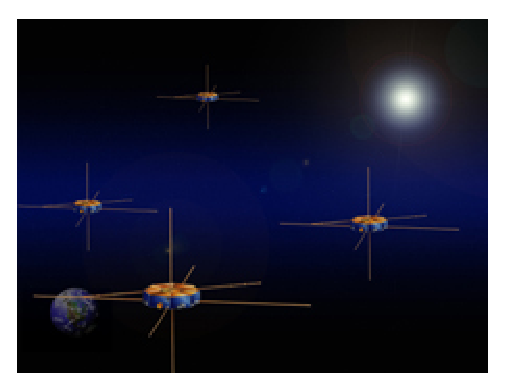
\psfig{file=figures/mms_spacecraft_formation.eps,height=1.2in}}
\caption{MMS Spacecraft Formation}
\label{fig:magneticfields}
\end{figure}

A reconnection event occurs when magnetic field lines cross allowing energetic particles to traverse from interstellar space into the Earth's magnetosphere releasing large quantities of heat and kinetic energy.  The diffusion region of a reconnection event starts on the day side magnetopause an quickly folds over to the Earth's magnetotail (Figure \ref{fig:magneticfields}).  This region is only 1-10 km in size but can travel at 10-100 km/hr \cite{swri} making it extremely difficult to measure.  Effects of a reconnection event are regularly experienced via the aurora borealis, interference with spacecraft GPS systems, and disruptions to electrical grids and communication networks.

\begin{figure}[H]
\centerline{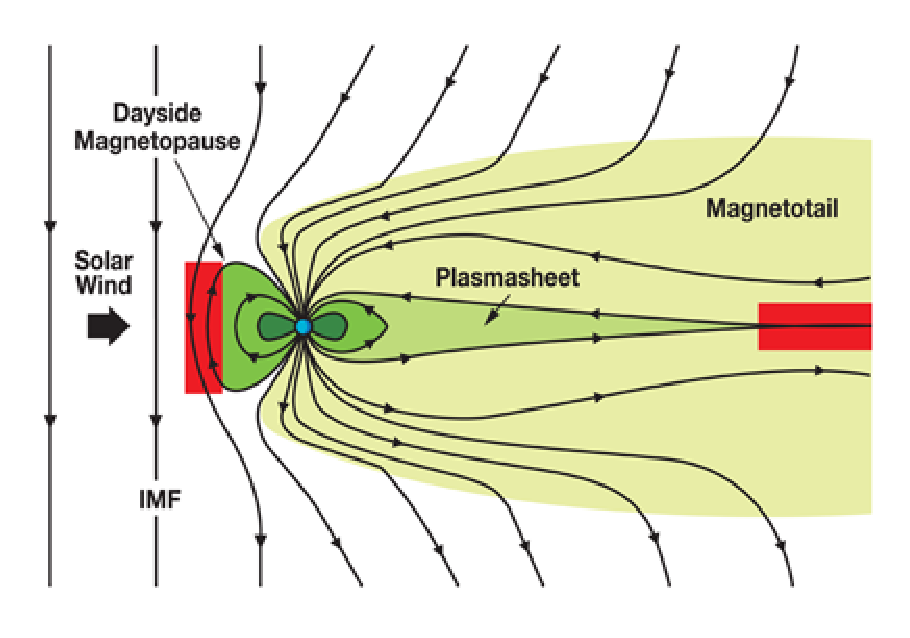
\psfig{file=figures/2d_earth_mag_field_lines.eps,height=1.2in}}
\caption{Earth's magnetic field}
\label{fig:magneticfields}
\end{figure}

Despite the widely experienced effects of reconnection events, very little about the microphysics inside its the diffusion region has been adequately measured.  Magnetometers, spectrometers, and other equipment currently in orbit are only able to capture a small fraction of the event's behavior.  Most equipment collect data from a single point or direction in space or some can get a 360 view of space by applying a slow spin to the spacecraft.  Both of these measurement methods are insufficient at capturing the structure of the diffusion region as it passes.

MMS's four satellites will be equipped with instrumentation mounted at the end of six boom extending out from the spacecraft's body along each major axis.  Four boom are the Spin Plane Double Probes (SDP) and two Axial Double Probes (ADP).  This configuration along with high resolution electron and ion spectrometers gives the constellation a new insight into the internal structure of the diffusion region.  The instrumentation at the ends of the boom are an advantage to the science portion of the mission, but create a unique challenge for the Attitude Determination and Control Systems (ADCS).  The satellites are spin stabilized at a rate of 3 rpm.  Disturbances to the rotation could translate into undesirable boom dynamics and nutations off the spin plane.



% Science questions to answer \cite{mms_website}
%     What determines when reconnection starts and how fast it proceeds?
%     What is the structure of the diffusion region?
%     How do the plasmas and magnetic fields disconnect and reconnect in the diffusion regions?
%     What role do the electrons play in facilitating reconnection?
%     What is the role of turbulence in the reconnection process?
%     How does reconnection lead to the acceleration of particles to high energies?


% \todo{image of formation flight}
% study microphysics of
%   magnetic reconnection
%   energetic particle acceleration
%   turbulence

% s/c MMS-1, MMS-2..MMS-4
% reconnection: Electromagnetic energy from the sun interacts with Earth's magnetosphere causing magnetic field lines to cross and create a burst of energy \cite{nasa_edge_video_ne_at_mms}
% magnetic reconnection measured ions and electrons as boundary passes to create 3d model of it passing by
% Fast plasma investigation
% probing the electron diffusion region (EDR) (passes too rapidly to get an accurate view with current equipment small (1-10 km) and rapidly moving (10-100 km/s))
% adjacent magnetic fields generally have significantly different orientations such that when they intersect, a large amount of energy is dispursed within a small region in the form of heat and kinetic energy.  The region = diffusion region
% explore magnetic reconnection
% dynamic regions of magnetosphere
% orbits planned to pass through the upstream and downstream magnetic reconnection sites
% 1) day side - solar wind field lines connection
% 2) down stream -
% 3) plasma travels down and causes the Arura
% through magnetospheric reconnection, portals allow energetic particles to traverse from outside to the interior of the magnetosphere
% predict when solar space weather within the magnetosphere and if they will affect orbiting satellites
% adverse space weather within the magnetosphere can negatively impact spacecraft system health GPS, induce disruptive current in electrical grids, communications, increased radiation exposure on trans-polar flights

% Difficult to understand
% magnetic boundary passes satellites quickly so has been hard to measure
% MMS has instruments to capture measurements
% Instruments mounted on all sides of the
% 8 sensors 1/30th sec instead of

% October 2014, Atlas five launch \cite{nasa_edge_video}

% Sensors
%   star sensor -> attitude
%   accelerometers -> $\Delta V$


% Fast Plasma Instrument (FPI) - controls
%   16 Dual Electron spectrometer (DES) Goddard built
%   16 Dual Ion Spectrometer (DIS) Japan *** built, hand delivered
%   180 degree and +- 22 degree measurement
%   30 millisec measurement rate 100x faster than previous missions entire view of sky
% FPI
%   despins data

% Instument Data processing Unit (IDPU) - brains of measurements
%   collects, compresses, transmits requested measurement data
%   configure while on mission

% booms
%   eight deployable booms
%   two 12.5m axial booms (electric field sensors)
%   four 60m wire booms
%   two 5m booms in spin plane for magnetometers
% rigid, wire, top/bottom booms
% important to keep consistent spin rate to get accurate estimates of boom location


% \section{Propulsion}

% types: solid propellents, bi propellents, electro propulsion, cold gas systems
% chose: mono-propellant blowdown - hydrozene power thrusters \cite{nasa_edge_video_propulsion}
% 3 rpm
% radial thrusters - spinning
% axial thrusters - prevent nutation

% concern:
% propulsion introduce distrubances

% 20 second pulses

% fuel limits by number of adjustments


% \section{performance requirements}

% $\pm 0.5$ deg attitude tollerance
% 1/10th of a second

\section{Research Objective}
\label{sec:ResearchObjective}

The work described in this thesis utilizes an experimental tabletop satellite (TableSat) \cite{vessthesis} to span three main efforts.  First is to create a physical model of a satellite from NASA's Magnetospheric MultiScale (MMS) Mission in order to validate and compare varied gyroless attitude determination and control (ADC) techniques.  The ADC systems must keep the TableSat rotating at a constant 3 rpm, prevent boom oscillations, and correct for detected nutations off the spin plane.  The second goal is to produce a software system that can be used to run against both theoretical simulations and experimental models.  The third goal is improve TableSat's use as an outreach tool.  The system should provide near ``real-time'' feedback of the system's state, allow for on-the-fly modification to control parameters, and be designed such that a individuals specializing in control systems could customize and extend its functionality without substantial computer science expertise.

\section{Past Work}
\label{sec:PastWork}

This work is a direct extension off of Vess' \cite{vessthesis} research using TableSat through Matlab Simulink and onboard flight controllers to demonstrate fundamentals of control theory.  The TableSat experimental design was modified to study the system dynamics of the instrument booms and nutation actuators in NASA's MMS mission satellites.  Previous experimental \cite{tsat1b} \cite{tsat1c} \cite{tsat2} and analytical \cite{mushawehthesis} ADC work at University of New Hampshire's Advanced Control Lab (ACL) has been done targeting the MMS mission.  The TableSat platform or similar derivations have also been adapted in investigate other areas of research including embedded systems development \cite{tablesat_xuml} and fault tolerant control \cite{tablesat_object_bench} \cite{nanjing_university}.


\section{Analytical and Experimental Testbed}
\label{sec:AnalyticalandExperimentalTestbed}



\section{Thesis Contributions}
\label{sec:ThesisContributions}

This research contributes to the field of feedback control, particularly as it relates to spin stabilized spacecraft, in the following ways:

\begin{itemize}
\item Gyroless observer-based controllers used to detect and eliminate nutations and maintain control of a spin stabilized satellite.
\item Improved capabilities of validating observer-based control methods by keeping identical control systems between analytical simulations and real experiments.
\item Allow clusters of estimators and controllers to all receive the same update for improved side-by-side comparisons of effectiveness.
\item Reduce time required to tune a controller by allowing for gain adjustments and swapping of estimation/control techniques on-the-fly.
\item Decompose quaternion state into separate rotational and nutation quaternions for use in error correction.
\item Use decomposed quaternion and differentiated rotational quaternions to decouple rate and attitude control.
\item Base quaternion state corrections on the representative rotational angle error, not the quaternion's sinusoidal scalar term.
\item Build the application such that the same control laws can be used to drive analytical simulations as well as experimental tests with physical systems.
\item Develop the application in a modular fashion to easily allow for future improvements and additions.
\item Control rates between modules such as sensors to estimators and estimators to controllers are independent and can operate at separate rates.
\item ``run-time'' feedback is available to visualize how the controller believes the system is responding.
\item A global clock instance is used for the authoritative time which during simulations can be adjusted in runtime to speed up or slow down the simulation to obtain better insight into the system dynamics.
\item Compensations for variable step sizes ($\delta t$) are made where able to protect the numerical integrity of the controller under large changes in control rates.
\item Code covered by proper software unit tests to validate and maintain expected behavior of the system during software upgrades.
\item Provide the combination of ``run-time'' visualizations and on-the-fly parameter/controller tuning for outreach programs.
\item Write the control application in a high level language to keep it accessible for improvements to control systems engineers with moderate programming experience.
\end{itemize}

\section{Thesis Outline}
\label{sec:ThesisOutline}



% %\include{notes/notes}
% %\include{appendices/appendices}

% %\include{appendices/bib}



% %\chapter{Equations}

% %\textbf{=============NOTES=============}
% %\include{equations/euler_body_rate}
% %\include{equations/quaternion_dynamics}
% %\include{equations/quaternion_body_rate}
% %\include{equations/quaternion_multiplication}
% %\include{equations/decompose_quaternion}
% %\include{quaternion/basics}
% %\textbf{=============NOTES=============}
% %\include{control/control_error}
% %\include{control/pid}

% %\include{Ch_TSat_Construction}

% % How is data aquired
% %\include{Ch_Data_aquisition}


% %Prior Versions - Matlab Code
% %\include{Ch_Prior_Versions}



% %Matlab Code
% %\include{Ch_Matlab_code}




% %Observer methods
% %\include{Ch_Observer_models}


% %\include{Ch_Controller_models}


% %\include{Ch_Observer_Control}


% %\chapter{Experimental Verification}
% %\label{chap:experimental}
% %\include{Ch_Experimental}



% %\chapter{Discussion of Results}
% %\label{chap:results}
% %\include{Ch_Results}

% %\chapter{Conclusions and Future Work}
% %\label{chap:conclusions}
% %\include{Ch_Conclustions}


% %\include{Appendix_Source_Code}
% %Matlab files
% %\chapter{Matlab Source Code}\label{ch:matlab_source}
% %\include{Matlab_Source_Code}

% \include{Bibliography}


% \newpage

% % \munfig{Credit: Southwest Research Institute}{mms_spacecraft_formation}{pretty/mms_spacecraft_formation.jpg}{0.4}

% % \munfig{Credit: http://earthobservatory.nasa.gov}{northern_lights_iss}{pretty/Northern-lights-ISS.jpg}{0.4}

% % \munfig{Credit: http://mms.gsfc.nasa.gov}{tetrahedron}{pretty/mms_dayside_tetrahedral_thumb.png}{0.4}

% % \munfig{Credit: http://mms.gsfc.nasa.gov}{2d_field_lines}{pretty/2d_earth_mag_field_lines.png}{0.4}
% % \munfig{Credit: http://mms.gsfc.nasa.gov}{instrument_deck_webview}{pretty/instrument_deck_webview.jpg}{0.4}
% % \munfig{Credit: http://mms.gsfc.nasa.gov}{observatory_dimensions1_webview}{pretty/observatory_dimensions1_webview.jpg}{0.4}
% % \munfig{Credit: http://mms.gsfc.nasa.gov}{observatory_interfaces_webview}{pretty/observatory_interfaces_webview.jpg}{0.4}
% % \munfig{Credit: http://mms.gsfc.nasa.gov}{observatory_webview}{pretty/observatory_webview.jpg}{0.4}

% % \munfig{Credits: ASRC Research and Technology/Barbara Lambert}{assembly}{pretty/713494main2_MMS-Observatory2-assembled-670.jpg}{0.4}

\end{document}